%%%%%%%%%%%%%%%%%%%%%%%%%%%%%%%%%%%%%%%%%%%%%%
%
%		My Thesis
%
%%%%%%%%%%%%%%%%%%%%%%%%%%%%%%%%%%%%%%%%%%%%%%

%%%%%%%%%%%%%%%%%%%%%%%%%%%%%%%%%%%%%%%%%%%%%%
%
%		Thesis Settings
%
%		EDOC Template
%		2011
%
%%%%%%%%%%%%%%%%%%%%%%%%%%%%%%%%%%%%%%%%%%%%%%
\pdfobjcompresslevel 0
\documentclass[a4paper,11pt]{book}
\usepackage{etex}

\usepackage[T1]{fontenc}
\usepackage[utf8]{inputenc}
\usepackage[french,english]{babel}


%%%%%%%%%%%%%%%%%%%%%%%%%%%%%%%%%%%%%%%%%%%%%%%
%% EDOC THESIS TEMPLATE: Variant 1.0 -> Latin modern, large text width&height
%%%%%%%%%%%%%%%%%%%%%%%%%%%%%%%%%%%%%%%%%%%%%%%
%\usepackage{lmodern}
%\usepackage[a4paper,top=22mm,bottom=28mm,inner=35mm,outer=25mm]{geometry}
%%%%%%%%%%%%%%%%%%%%%%%%%%%%%%%%%%%%%%%%%%%%%%%

%%%%%%%%%%%%%%%%%%%%%%%%%%%%%%%%%%%%%%%%%%%%%%
% EDOC THESIS TEMPLATE: Variant 2.0 -> Utopia, Gabarrit A (lighter pages)
%%%%%%%%%%%%%%%%%%%%%%%%%%%%%%%%%%%%%%%%%%%%%%
\usepackage{fourier} % Utopia font-typesetting including mathematical formula compatible with newer TeX-Distributions (>2010)
%\usepackage{utopia} % on older systems -> use this package instead of fourier in combination with mathdesign for better looking results
%\usepackage[adobe-utopia]{mathdesign}
\setlength{\textwidth}{140mm} % = 210mm - 37mm - 26.2mm
\setlength{\oddsidemargin}{14mm} % 37mm - 1in (from hoffset)
\setlength{\evensidemargin}{5mm} % = 26.2mm - 1in (from hoffset)
\setlength{\topmargin}{0mm} % = 0mm -1in + 23.2mm 
\setlength{\textheight}{215mm} % = 297mm -29.5mm -31.6mm - 14mm (12 to accomodate footline with pagenumber)
\setlength{\headheight}{15pt}
%%%%%%%%%%%%%%%%%%%%%%%%%%%%%%%%%%%%%%%%%%%%%%



\setlength{\parindent}{0pt}

\usepackage{setspace} % increase interline spacing slightly
\setstretch{1.05}

\makeatletter
\setlength{\@fptop}{0pt}  % for aligning all floating figures/tables etc... to the top margin
\makeatother


\usepackage{graphicx,xcolor}
\graphicspath{{images/}}

\usepackage{subfig}
\usepackage{booktabs}
\usepackage{lipsum}
\usepackage{microtype}
\usepackage{url}
\usepackage[final]{pdfpages}
\usepackage{pict2e}

\usepackage{fancyhdr}
\renewcommand{\sectionmark}[1]{\markright{\thesection\ #1}}
\pagestyle{fancy}
	\fancyhf{}
	\renewcommand{\headrulewidth}{0.4pt}
	\renewcommand{\footrulewidth}{0pt}
	\fancyhead[OR]{\bfseries \nouppercase{\rightmark}}
	\fancyhead[EL]{\bfseries \nouppercase{\leftmark}}
	\fancyfoot[EL,OR]{\thepage}
\fancypagestyle{plain}{
	\fancyhf{}
	\renewcommand{\headrulewidth}{0pt}
	\renewcommand{\footrulewidth}{0pt}
	\fancyfoot[EL,OR]{\thepage}}
\fancypagestyle{addpagenumbersforpdfimports}{
	\fancyhead{}
	\renewcommand{\headrulewidth}{0pt}
	\fancyfoot{}
	\fancyfoot[RO,LE]{\thepage}
}


\usepackage{amsmath}

\usepackage{listings}
\lstset{language=[LaTeX]Tex,tabsize=4, basicstyle=\scriptsize\ttfamily, showstringspaces=false, numbers=left, numberstyle=\tiny, numbersep=10pt, breaklines=true, breakautoindent=true, breakindent=10pt}

\usepackage[hyperindex=true,hypertexnames=false]{hyperref} % second parameter enable to have the right hyperlink in the french introduction (reset chapter number)
\hypersetup{pdfborder={0 0 0},
	colorlinks=true,
	linkcolor=black,
	citecolor=EmphCite,
	urlcolor=black}
\urlstyle{same}

\makeatletter
\def\cleardoublepage{\clearpage\if@twoside \ifodd\c@page\else
    \hbox{}
    \thispagestyle{empty}
    \newpage
    \if@twocolumn\hbox{}\newpage\fi\fi\fi}
\makeatother \clearpage{\pagestyle{plain}\cleardoublepage}


\usepackage{color}
\usepackage{tikz}
\usepackage{pgfplots}
\usetikzlibrary{positioning}


%%%%% CHAPTER HEADER %%%%
\usepackage[explicit]{titlesec}
\newcommand*\chapterlabel{}
%\renewcommand{\thechapter}{\Roman{chapter}}
\titleformat{\chapter}[display]  % type (section,chapter,etc...) to vary,  shape (eg display-type)
	{\normalfont\bfseries\Huge} % format of the chapter
	{\gdef\chapterlabel{\thechapter\ }}     % the label 
 	{0pt} % separation between label and chapter-title
 	  {\begin{tikzpicture}[remember picture,overlay]
    \node[yshift=-8cm] at (current page.north west)
      {\begin{tikzpicture}[remember picture, overlay]
        \draw[fill=PartChapter] (0,0) rectangle(35.5mm,15mm);
        \node[anchor=north east,yshift=-7.2cm,xshift=34mm,minimum height=30mm,inner sep=0mm] at (current page.north west)
        {\parbox[top][30mm][t]{15mm}{\raggedleft $\phantom{\textrm{l}}$\color{white}\chapterlabel}};  %the black l is just to get better base-line alingement
        \node[anchor=north west,yshift=-7.2cm,xshift=39mm,text width=\textwidth,minimum height=30mm,inner sep=0mm] at (current page.north west)
              {\parbox[top][30mm][t]{\textwidth}{\color{black}#1}};
       \end{tikzpicture}
      };
   \end{tikzpicture}
   \gdef\chapterlabel{}
  } % code before the title body

\titlespacing*{\chapter}{0pt}{50pt}{30pt}
\titlespacing*{\section}{0pt}{10.2pt}{*0}  % 13.2pt is line spacing for a text with 11pt font size
\titlespacing*{\subsection}{0pt}{13.2pt}{*0}
\titlespacing*{\subsubsection}{0pt}{13.2pt}{*0}

\newcounter{myparts}
\newcommand*\partlabel{}
\titleformat{\part}[display]  % type (section,chapter,etc...) to vary,  shape (eg display-type)
	{\normalfont\bfseries\Huge} % format of the part
	{\gdef\partlabel{\thepart\ }}     % the label 
 	{0pt} % separation between label and part-title
 	  {\setlength{\unitlength}{20mm}
	  \addtocounter{myparts}{1}
	  \begin{tikzpicture}[remember picture,overlay]
    \node[anchor=north west,xshift=-65mm,yshift=-6.9cm-\value{myparts}*0mm] at (current page.north east) % for unknown reasons: 3mm missing -> 65 instead of 62
      {\begin{tikzpicture}[remember picture, overlay]
        \draw[fill=PartChapter] (0,0) rectangle(62mm,20mm);   % -\value{myparts}\unitlength
        \node[anchor=north west,yshift=-6.1cm-\value{myparts}*0mm,xshift=-60.5mm,minimum height=30mm,inner sep=0mm] at (current page.north east)
        {\parbox[top][30mm][t]{55mm}{\raggedright \color{white}Part \partlabel $\phantom{\textrm{l}}$}};  %the phantom l is just to get better base-line alingement
        \node[anchor=north east,yshift=-6.1cm-\value{myparts}*0mm,xshift=-63.5mm,text width=\textwidth,minimum height=30mm,inner sep=0mm] at (current page.north east)
              {\parbox[top][30mm][t]{\textwidth}{\raggedleft \color{black}#1}};
       \end{tikzpicture}
      };
   \end{tikzpicture}
   % \vfil\center{\@partimage}%\vfil%\hfil%\endgroup 
   \gdef\partlabel{}
  } % code before the title body

% Fix the problem with delimiter size caused by fourier and amsmath packages.
\makeatletter
\def\resetMathstrut@{%
  \setbox\z@\hbox{%
    \mathchardef\@tempa\mathcode`\(\relax
      \def\@tempb##1"##2##3{\the\textfont"##3\char"}%
      \expandafter\@tempb\meaning\@tempa \relax
  }%
  \ht\Mathstrutbox@1.2\ht\z@ \dp\Mathstrutbox@1.2\dp\z@
}
\makeatother


%%%%%%%%%%%%%%%%%%%%%%%%%%%%%%%%%%%%%%%%%%%%%%
%
%		Thesis Settings
%		Custom settings
%
%		2011
%
%%%%%%%%%%%%%%%%%%%%%%%%%%%%%%%%%%%%%%%%%%%%%%
%\usepackage{empheq} 
\usepackage{supertabular} 
%\usepackage[numbers,sort&compress]{natbib}
\usepackage{bibentry}

% Three next lines enable to use footnotes in tabular
\usepackage{footnote}
\makesavenoteenv{tabular}
\makesavenoteenv{table}

\usepackage{enumitem}
\setlist[enumerate]{topsep=0pt,itemsep=-1ex,partopsep=1ex,parsep=1ex}
\setlist[itemize]{topsep=0pt,itemsep=-1ex,partopsep=1ex,parsep=1ex}

\usepackage{siunitx}
%\usepackage{algorithm}
%\usepackage{algorithmic}

\newenvironment{changemargin}[2]{\begin{list}{}{%
\setlength{\topsep}{0pt}%
\setlength{\leftmargin}{0pt}%
\setlength{\rightmargin}{0pt}%
\setlength{\listparindent}{\parindent}%
\setlength{\itemindent}{\parindent}%
\setlength{\parsep}{0pt plus 1pt}%
\addtolength{\leftmargin}{#1}%
\addtolength{\rightmargin}{#2}%
}\item }{\end{list}}

%%-------------------------------
% Center in title line
%%-------------------------------
\newcommand*{\thead}[1]{\multicolumn{1}{c}{#1}}


%%-------------------------------
% Enable to specify that a \part is finished
%%-------------------------------
\usepackage{bookmark}
% To specify the end of a part, add the following commands
% \bookmarksetup{startatroot}% this is it
% \addtocontents{toc}{\bigskip}% perhaps as well

%%-------------------------------
% Colors
%%-------------------------------
\usepackage{xcolor}
\definecolor{bottle green}{RGB}{9, 106, 9}
\definecolor{kaki}{rgb}{.5,.5,0}

\definecolor{argon orange}{RGB}{237, 128, 0}  % Argon orange
\definecolor{argon gray}{RGB}{83, 86, 90}     % Argon gray

\definecolor{PartChapter}{RGB}{237, 128, 0}
\definecolor{EmphCite}{RGB}{83, 86, 90}
%\definecolor{darkgrey}{HTML}{2E2E2E}
%\definecolor{darkgrey2}{HTML}{585858}
%\definecolor{lightgrey2}{HTML}{A4A4A4}
%\definecolor{lightgrey}{HTML}{D8D8D8}

\newcommand{\red}[1]{\textcolor{red}{#1}}
\newcommand{\maincolor}[1]{\textcolor{argon orange}{#1}}
\newcommand{\secondcolor}[1]{\textcolor{argon gray}{#1}}
%\newcommand{\blue}[1]{\begin{color}{bleuEmphCite}\textit{#1}\end{color}}



% Put emphasized text in color
%\let\oldemph\emph
%\renewcommand\emph[1]{{\color{bleuEmphCite}\oldemph{#1}}}

%%-------------------------------
% Image on part pages
%%-------------------------------
\newcommand{\partimage}[2][]{\gdef\@partimage{\includegraphics[#1]{#2}}}

%%-------------------------------
% Index
%%-------------------------------
% \usepackage{makeidx}
% \makeindex

\usepackage{imakeidx}
\indexsetup{othercode=\small}
\makeindex[program=makeindex,columns=2,options={-s head/index_style.ist}]
% \makeindex[options= -s head/index_style.ist]



%%%%%%%%%%%%%%%%%%%%%%%%%%%%%%%%%%%%%%%%%%%%%%%%%%
%% for interactions
\usepackage{todonotes}
\newcommand{\vl}[1]{\todo[color=blue!50]{#1}}
\newcommand{\esg}[1]{\todo[color=green!50]{#1}}
\newcommand{\fm}[1]{\todo[color=red!50]{#1}}
\newcommand{\vlil}[1]{\todo[inline,color=blue!20]{VL: #1}}
\newcommand{\esgil}[1]{\todo[inline,color=green!20]{ESG: #1}}
\newcommand{\fmil}[1]{\todo[inline,color=red!20]{FM: #1}}
%%%%%%%%%%%%%%%%%%%%%%%%%%%%%%%%%%%%%%%%%%%%%%%%%%%%%%%%%%%%



%%%%%%%%%%%%%%%%%%%%%%%%%%%%%%%%%%%%%%%%%%%%%%
%
%		Thesis Commands
%
%%%%%%%%%%%%%%%%%%%%%%%%%%%%%%%%%%%%%%%%%%%%%%

% Correct mathcal letters
\DeclareSymbolFont{calletters}{OMS}{cmsy}{m}{n}
\DeclareSymbolFontAlphabet{\mathcal}{calletters}

% To include images
\usepackage{graphicx}

% More maths and chemistry
\usepackage{amsmath,amssymb,amsfonts,amsthm,dsfont,stmaryrd}
\usepackage[overload]{empheq}
\usepackage[version=3]{mhchem} % chemistry
%\usepackage{physics}  % Physics
\usepackage{siunitx}  % International System of Units (SI).
\usepackage{eurosym}  % Euro symbol

% Environnement outdent (centre)
\newenvironment{outdent}
{\begin{list}{}{\leftmargin-2cm\rightmargin\leftmargin}\centering\item\relax}
{\end{list}\ignorespacesafterend}

% Environnement PROBLEME
\newenvironment{probleme}[1]{\vskip 0.12 cm\noindent{\bf {\sc
#1}}}{\vspace*{0.12 cm}}
\newcommand{\inputProblem}{\newline\noindent{\bf Input.~}}
\newcommand{\outputProblem}{\newline\noindent{\bf Output.~}}

\newcommand{\inputProblemfr}{\newline\noindent{\bf Entrée.~}}
\newcommand{\outputProblemfr}{\newline\noindent{\bf Sortie.~}}

%------------------------ Theorems
%\usepackage{amsmath,amssymb,amsthm}
\usepackage{cleveref}
\usepackage{thmtools}
\usepackage{thm-restate}
\usepackage{multirow}
\usepackage{pict2e}


\theoremstyle{plain}
\newtheorem{thm}{Theorem}
\newtheorem{lem}[thm]{Lemma}
\newtheorem{claim}[thm]{Claim}
\newtheorem{prop}[thm]{Proposition}
\newtheorem{cor}[thm]{Corollary}

\theoremstyle{definition}
\newtheorem{defn}{Definition}
\newtheorem{conj}{Conjecture}
\newtheorem{example}{Example}
\newtheorem{question}{Question}

\theoremstyle{remark}
\newtheorem{rmq}{Remark}

% fixes space after and before \left and \right
\let\originalleft\left
\let\originalright\right
\def\left#1{\mathopen{}\originalleft#1}
\def\right#1{\originalright#1\mathclose{}}

% Algorithms
\usepackage[english]{algorithm2e}
\SetKw{And}{and}
\SetKw{From}{from}
\SetKw{To}{to}
\setlength{\algomargin}{0em}

% Array environment
\usepackage{array} % Center tabular
\usepackage{multirow} % multirow and multicolumn
\usepackage{arydshln} % dashed line
%\usepackage[hang, small,labelfont=bf,up,textfont=it,up]{caption} % custom table names
\usepackage{booktabs} % Tables with lines

% Tikzpicture
\usepackage{tikz}
\usetikzlibrary{calc,arrows,automata,matrix,positioning,fit}
\usetikzlibrary{decorations,decorations.pathreplacing}
\usetikzlibrary{patterns}
\usepackage{tikzscale}
\usepackage{pgfplots}

% allows line breaks in \cite
\usepackage{cite}

% Useful shortcut
\newcommand{\tbc}{\red{\texttt{To be completed}}}
%\newcommand{\todo}[1]{\red{(TO DO: #1)}}
\def\ds{\displaystyle}
\newcommand{\ie}{\emph{i.e.}~}
\newcommand{\eg}{\emph{e.g.}~}
\newcommand{\NP}{NP}
\newcommand{\st}{\text{s.t.}}


%%%%%%%%%%%%%%%%%%%%%%%%%%%%%%%%%%%%%%%%%%%%%%%%%%%%%%%%%%%%%%%%%%%%
%%%%%                   Mathematic commands                    %%%%%
%%%%%%%%%%%%%%%%%%%%%%%%%%%%%%%%%%%%%%%%%%%%%%%%%%%%%%%%%%%%%%%%%%%%

\newcommand{\cA}{\mathcal{A}}
\newcommand{\cB}{\mathcal{B}}
\newcommand{\cC}{\mathcal{C}}
\newcommand{\cD}{\mathcal{D}}
\newcommand{\cE}{\mathcal{E}}
\newcommand{\cF}{\mathcal{F}}
\newcommand{\cG}{\mathcal{G}}
\newcommand{\cH}{\mathcal{H}}
\newcommand{\cI}{\mathcal{I}}
\newcommand{\cJ}{\mathcal{J}}
\newcommand{\cK}{\mathcal{K}}
\newcommand{\cL}{\mathcal{L}}
\newcommand{\cM}{\mathcal{M}}
\newcommand{\cN}{\mathcal{N}}
\newcommand{\cO}{\mathcal{O}}
\newcommand{\cP}{\mathcal{P}}
\newcommand{\cQ}{\mathcal{Q}}
\newcommand{\cR}{\mathcal{R}}
\newcommand{\cS}{\mathcal{S}}
\newcommand{\cT}{\mathcal{T}}
\newcommand{\cU}{\mathcal{U}}
\newcommand{\cV}{\mathcal{V}}
\newcommand{\cW}{\mathcal{W}}
\newcommand{\cX}{\mathcal{X}}
\newcommand{\cY}{\mathcal{Y}}
\newcommand{\cZ}{\mathcal{Z}}

\newcommand{\BB}{\mathbb{B}}
\newcommand{\CC}{\mathbb{C}}
\newcommand{\DD}{\mathbb{D}}
\newcommand{\EE}{\mathbb{E}}
\newcommand{\FF}{\mathbb{F}}
\newcommand{\GG}{\mathbb{G}}
\newcommand{\HH}{\mathbb{H}}
\newcommand{\II}{\mathbb{I}}
\newcommand{\JJ}{\mathbb{J}}
\newcommand{\KK}{\mathbb{K}}
\newcommand{\LL}{\mathbb{L}}
\newcommand{\MM}{\mathbb{M}}
\newcommand{\NN}{\mathbb{N}}
\newcommand{\OO}{\mathbb{O}}
\newcommand{\PP}{\mathbb{P}}
\newcommand{\QQ}{\mathbb{Q}}
\newcommand{\RR}{\mathbb{R}}
\newcommand{\TT}{\mathbb{T}}
\newcommand{\UU}{\mathbb{U}}
\newcommand{\VV}{\mathbb{V}}
\newcommand{\WW}{\mathbb{W}}
\newcommand{\XX}{\mathbb{X}}
\newcommand{\YY}{\mathbb{Y}}
\newcommand{\ZZ}{\mathbb{Z}}


%%%%% Bracket, square bracket and curly bracket with adaptation to the size of content
\newcommand{\bracket}[1]{\left(#1\right)}
\newcommand{\sqbracket}[1]{\left[#1\right]}
\newcommand{\crbracket}[1]{\left\{#1\right\}}

%%%%% Norm
\newcommand{\norm}[1]{\left\|#1\right\|}

%%%%% Fonction indicatrice
\newcommand{\findi}[1]{\mathbf{1}_{#1}}

%%%%% Integer interval
% If the lower bound is not specified, it assumes 1.
\makeatletter
\def\range{\@ifnextchar[{\@with}{\@without}}
\def\@with[#1]#2{\left\{#1,\ldots,#2\right\}}
\def\@without#1{\sqbracket{#1}}
\makeatother

%%%%% Cardinal of a set
\newcommand{\card}[1]{\left\vert{#1}\right\vert}

%%%%% Probability
\newcommand{\espe}{\mathbb{E}}                  % Mean
\newcommand{\prob}{\mathbb{P}}                  % Probability
\newcommand{\vari}{\mathrm{Var}}                % Variance
\newcommand{\VaR}{\mathrm{V@R}}                 % Value-at-risk
\newcommand{\AVaR}{\mathrm{A\VaR}}              % Average value-at-risk
\newcommand{\Sfield}[1]{\sigma\left(#1\right)}  % sigma-field generated by the random variable #1

%%%%% Differential
\newcommand{\diff}{\mathrm{d}}  % Differential

%%%%% Random variable
\makeatletter
\def\va@a{\boldsymbol{\va@arg^{\textstyle\text{\unboldmath$\scriptstyle\va@expo$}}_{\textstyle\text{\unboldmath$\scriptstyle\va@index$}}}}
\def\va#1{\def\va@expo{}\def\va@index{}\def\va@arg{#1}%
  \@ifnextchar^{\va@h}{\@ifnextchar_\va@u\va@a}}
\def\va@h^#1{\def\va@expo{#1}\@ifnextchar_\va@hu\va@a}
\def\va@u_#1{\def\va@index{#1}\@ifnextchar^\va@uh\va@a}
\def\va@hu_#1{\def\va@index{#1}\va@a}
\def\va@uh^#1{\def\va@expo{#1}\va@a}
\makeatother


%%%%%%%%%%%%%%%%%%%%%%%%%%%%%%%%%%%%%%%%%%%%%%%%%%%%%%%%%%%%%%%%%%%%
%%%%%                                                          %%%%%
%%%%% Variables                                                %%%%%
%%%%%                                                          %%%%%
%%%%%%%%%%%%%%%%%%%%%%%%%%%%%%%%%%%%%%%%%%%%%%%%%%%%%%%%%%%%%%%%%%%%

% Common
\newcommand\REF{\cI}  % Set of product


% PP modeling
\newcommand\horizon{T}              % Number of periods
\newcommand\cover{\tau}             % Cover for a product
\newcommand\coverset{\cT}           % Set of possible cover for a product
\newcommand\lot{\ell}               % lot of the product 
\newcommand\freq{n}                 % frequency of production
\newcommand\demand{d}               % Demand
\newcommand\cumdemand{D}            % Cumulative demand
\newcommand\holding{h}              % holding cost of product
\newcommand\backorder{\gamma}       % Backorder cost
\newcommand\capacity{C}             % Capacity of the assembly line
\newcommand\rate{v}                 % Capacity needed for assembly line to produce one unit of product
\newcommand\internal{v}             % Internal production time (time needed to produce one unit)
\newcommand\nbsetups{N}             % Total number of setups of the line
\newcommand\scenarios{\Omega}       % Set of scenarios

\newcommand\setup{x}                % 1 if product is produced at period and 0 otherwise
\newcommand\quantity{q}             % Quantity of product produced at period
\newcommand\inventory{s}            % Inventory of product at the end of period
\newcommand\backlog{b}              % Backlog quantity of product at end of period
\newcommand\level{\tilde{s}}        % Relative inventory of product at the end of period (may be negative)
\newcommand\supplied{\tilde{d}}     % Supplied demand
\newcommand\safety{s_{\min}}        % Safety stock of the product
\newcommand\lag{\tau}               % Number of periods for which decisions are fixed


% Strategic modeling
\newcommand\plants{\cP}       % Set of factories
\newcommand\capital{K}        % Available capital to invest in flexible production capacities
\newcommand\affect{c}         % Cost for assigning the capactity of production to a factory
\newcommand\produce{p}        % Cost for producing one unit of a product
\newcommand\assign{y}         % 1 if factory can produce product and 0 otherwise
\newcommand\open{z}           % 1 if factory got the ability to produce during previous period and 0 otherwise
\newcommand\servicelvl{\beta} % Service shortage (1 - service level)


%%%%%%%%%%%%%%%%%%%%%%%%%%%%%%%%%%%%%%%%%%%%%%
%%%%% HEAD
%%%%%%%%%%%%%%%%%%%%%%%%%%%%%%%%%%%%%%%%%%%%%%
\begin{document}

\frontmatter
\begin{titlepage}


% - - - - - - - début de la page 
\thispagestyle{empty}
\begin{center}

\includegraphics[width=9cm]{head/logo_upe.png}


\vspace*{0.5cm}

{\large \'Ecole doctorale {\sc Math\'ematiques et Sciences et Technologies de l'Information et de la Communication}}

\vspace*{1cm}

{\huge {\sc Th\`ese de doctorat}}

\vspace*{0.5cm}

{\large Sp\'ecialit\'e : Math\'ematiques}

\vspace*{1cm}

{\large Pr\'esent\'ee par}\ \\[1ex]

{\huge {Etienne \sc Gaillard de Saint Germain}}

\vspace*{1cm}

{\large Pour obtenir le grade de \ \\[1ex]
{\sc Docteur de l'Universit\'e Paris-Est}}

\vspace*{1.2cm}

{\Huge \maincolor{\sc To Be Completed}}

\vspace*{0.3cm}

{\Huge \maincolor{\sc ...}}

\vspace*{0.5cm}

{\large \maincolor{\sc ...}}

\vspace*{1.5cm}

{\Large Soutenance le 17 d\'ecembre 2018 devant le jury compos\'e de :}

\end{center}

\begin{tabular}{lll}
{\Large M. Jean-Philippe  {\sc Gayon}} & {\large{\it Affiliation}} & {\large Rapporteur}\\[0.5ex]
{\Large Mme Safia         {\sc Kedad-Sidhoum}} & {\large{\it CNAM}} & {\large Rapporteur}\\[0.5ex]
{\Large Mme Nadia         {\sc Brauner}} & {\large{\it Universit\'e Grenoble Alpes}} & {\large Examinateur}\\[0.5ex]
%{\Large M. Chengbin       {\sc Chu}} & {\large{\it Affiliation}} & {\large Examinateur}\\[0.5ex]
{\Large Mme C\'eline      {\sc Gicquel}} & {\large{\it Universit\'e Paris Sud}} & {\large Examinateur}\\[0.5ex]
{\Large M. Fabrice        {\sc Bonneau}} & {\large{\it Argon Consulting}} & {\large Encadrant de th\`ese}\\[0.5ex]
{\Large M. Vincent        {\sc Lecl\`ere}} & {\large{\it \'Ecole des Ponts ParisTech}} & {\large Encadrant de th\`ese}\\[0.5ex]
{\Large M. Fr\'ed\'eric   {\sc Meunier}} & {\large{\it \'Ecole des Ponts ParisTech}} & {\large Directeur de th\`ese}

\end{tabular}

\end{titlepage}
\setcounter{page}{0}
\cleardoublepage

\begin{titlepage}
\vspace*{5cm}

\begin{flushright}\`A Papa\end{flushright}

\end{titlepage}
\setcounter{page}{0}
\cleardoublepage

\setlength{\parskip}{0.6em}	

\addcontentsline{toc}{chapter}{Remerciements}
\chapter*{Remerciements} % (fold)
\label{cha:remerciements}

\tbc


\addcontentsline{toc}{chapter}{Abstract}
\chapter*{Abstract} % (fold)
\label{cha:abstract}



This thesis develops optimization methods for Supply Chain Management and are centered around the flexibility which is the ability to deliver a service or a product to a costumer although the environment and the future is uncertain.
The research were conducted throughout partnership between Argon consulting which is an independent consulting firm in Supply Chains Operations and the \'Ecole des Ponts ParisTech.
In this thesis, we explore three topics that are encountered by Argon Consulting and its clients and that correspond to three different levels of decision (long-term, mid-term and short-term).


When companies expand their product portfolio, they must decide where produce each item.
This is a long-term decision since once it is decided, it cannot be be easily changed.
More than a assignment problem where one item is produced by a single plant, the objective of this problem is to decide if some items should be produced on several plants and by which plants.
Indeed, demand for items is highly uncertain.
So, in order to satisfy the demand, the assignment must be able to balance the workload between plants.
This problem is called multi-sourcing of production.
Since it is not a repeated problem, it is essential to take into account the risk aversion when making the multi-sourcing decision.
We propose a generic model that includes the technical constraints of the assignment and a risk-averse constraint based on risk measures from the financial applications.
We develop an algorithm and a heuristic based on standard tools from Operational Research and Stochastic Optimization to solve the multi-sourcing problem and test the efficiency on real datasets.


Before planning the production, some macroscopic indicators must be decided at mid-term level such that the quantity of raw materials to order or the size of produced batches.
Continuous-time inventory models are used by some companies but they often rely on a trade-off between holding costs and setups costs that are fixed costs paid when production is launched and that are hard to estimate in practice.
On the other hand, at mid-term level, flexibility of the mean of production is already fixed and companies easily estimate the maximal number of setups.
We propose extensions of some classical continuous-time inventory models taking into account this bound on the number of setups.
We used standard tools from Continuous Optimization to compute the optimal macroscopic indicators.


Finally, planning the production is a short-term decision consisting in deciding which items must be produced by the assembly line during the current period.
This problem belong to the well-studied class of Lot-Sizing Problems.
As for mid-term decisions, these problems often rely on a trade-off between holding and setup costs.
Basing our model on industrial consideration, we propose a new model replacing setup costs by a bound on the number of setups for each period of production.
Although this are short-term decision, production decisions must take into account future demand which remains uncertain.
So, we solve our production planning problem using standard tools from Operational Research and Stochastic Optimization, test the efficiency on real datasets and compare it to heuristic used by Argon Consulting's clients.


\secondcolor{Key words}: Supply Chain Management, Operational Research, Stochastic Optimization, Lot-Sizing, Assignment problem, risk measure, heuristics.


\addcontentsline{toc}{chapter}{Résumé}
\chapter*{R\'esum\'e} % (fold)
\label{cha:resume}


Cette thèse développe des méthodes d'optimisation pour la gestion de la Supply Chain et a pour thème central la flexibilité définie comme la capacité à fournir un service ou un produit au consommateur dans un environnement incertain.
La recherche a été menée dans le cadre d'une convention CIFRE entre Argon Consulting, une société indépendante de conseil en Supply Chain et l'\'Ecole des Ponts ParisTech.
Dans cette thèse, nous développons trois sujets rencontrés par Argon Consulting et ses clients et qui correspondent à trois différents niveaux de décision (long terme, moyen terme et court terme).


Lorsque les entreprises élargissent leur portefeuille de produits, elles doivent décider dans quelles usines produire chaque article.
Il s'agit d'une décision à long terme, car une fois qu'elle est prise, elle ne peut être facilement modifiée.
Plus qu'un problème d'affectation où un article est produit par une seule usine, ce problème consiste à décider si certains articles doivent être produits par plusieurs usines et par lesquelles.
Cette interrogation est motivée par la grande incertitude de la demande.
En effet, pour satisfaire la demande, l'affectation doit pouvoir équilibrer la charge de travail entre les usines.
Nous appelons ce problème le multi-sourcing de la production.
Comme il ne s'agit pas d'un problème récurrent, il est essentiel de tenir compte du risque au moment de décider le niveau de multi-sourcing.
Nous proposons un modèle générique qui inclut les contraintes techniques du problème et une contrainte d'aversion au risque basée sur des mesures de risque issues de la théorie financière.
Nous développons un algorithme et une heuristique basés sur les outils standards de la Recherche Opérationnelle et de l'Optimisation Stochastique pour résoudre le problème du multi-sourcing et nous testons leur efficacité sur des données réelles.


Avant de planifier la production, certains indicateurs macroscopiques doivent être décidés à horizon moyen terme tels la quantité de matières premières à commander ou la taille des lots produits.
Certaines entreprises utilisent des modèles de stock en temps continu, mais ces modèles reposent souvent sur un compromis entre les coûts de stock et les coûts de lancement.
Ces derniers sont des coûts fixes payés au lancement de la production et sont difficiles à estimer en pratique.
En revanche, à horizon moyen terme, la flexibilité des moyens de production est déjà fixée et les entreprises estiment facilement le nombre maximal de lancements.
Poussés par cette observation, nous proposons des extensions de certains modèles classiques de stock en temps continu, sans coût de lancement et avec une limite sur le nombre d'installations.
Nous avons utilisé les outils standard de l'Optimisation Continue pour calculer les indicateurs macroscopiques optimaux.


Enfin, la planification de la production est une décision à court terme qui consiste à décider quels articles doivent être produits par la ligne de production pendant la période en cours.
Ce problème appartient à la classe bien étudiée des problèmes de Lot-Sizing.
Comme pour les décisions à moyen terme, ces problèmes reposent souvent sur un compromis entre les coûts de stock et les coûts de lancement.
Fondant notre modèle sur ces considérations industrielles, nous gardons le même point de vue (aucun coût de lancement et une borne supérieure sur le nombre de lancement) et proposons un nouveau modèle.
Bien qu'il s'agisse de décisions à court terme, les décisions de production doivent tenir compte de la demande future, qui demeure incertaine.
Nous résolvons notre problème de planification de la production à l'aide d'outils standard de Recherche Opérationnelle et d'Optimisation Stochastique, nous testons l'efficacité sur des données réelles et nous la comparons aux heuristiques utilisées par les clients d'Argon Consulting.



\secondcolor{Mots-clés} : Heuristique, Lot-Sizing, Mesure de Risque, Optimisation Stochastique, Problème d'affectation, Recherche Opérationnelle, Supply Chain Management.


\setlength{\parskip}{0em}	

\addtocontents{toc}{\protect{\pdfbookmark[0]{\contentsname}{toc}}}
\tableofcontents
\cleardoublepage
\phantomsection
\addcontentsline{toc}{chapter}{List of figures}
\listoffigures
\cleardoublepage
\phantomsection
\addcontentsline{toc}{chapter}{List of tables}
\listoftables

\setlength{\parskip}{0.6em}	


%%%%%%%%%%%%%%%%%%%%%%%%%%%%%%%%%%%%%%%%%%%%%%
%%%%% Remove these lines
%%%%% Only to quickly compile figures to test them
%%%%%%%%%%%%%%%%%%%%%%%%%%%%%%%%%%%%%%%%%%%%%%
% \cleardoublepage
% % \begin{figure}[h]
%   \centering
%   \includegraphics[width=\textwidth]{main/introduction/images/supply_chain_models.tikz}
%   \caption{Supply Chain organizations and lead times (from \cite{Arnold2007})}
%   \label{fig:supply-chain-models}
% \end{figure}


% \begin{figure}[h]
%   \centering
%   \includegraphics[width=\textwidth]{main/introduction/images/inventory_decomposition.tikz}
%   \caption{Inventory decomposition}
%   \label{fig:inventory-decomposition}
% \end{figure}






%%%%%%%%%%%%%%%%%%%%%%%%%%%%%%%%%%%%%%%%%%%%%%
%%%%% MAIN
%%%%%%%%%%%%%%%%%%%%%%%%%%%%%%%%%%%%%%%%%%%%%%
\mainmatter
\chapter{Introduction}


Hello world!


%!TEX root=../../thesis_ESG.tex
\chapter{Business context}
\label{chap:business-context}


A Supply Chain is a system of organizations, people, activities, information, and resources involved in producing, transforming or moving a product or service from supplier to customer.
It can be considered for a subsidiary, a whole company or for multiple companies working together.
Its activities extends from the recovery of raw material to their transformation into finished product and their delivery to the costumer.

Supply Chain can fulfill several functions.
Most common are procurement, production, distribution, storage, shipping, sales and billing, and customer relationship.
Works of this thesis deal with optimization of production and storage within companies.


\section{Supply Chain objectives}



Supply Chain management consists in finding the right balance between conflicting objectives.
%Customer satisfaction is based on a trade-off between low cost, appropriate and quality product or service and short delivery lead time.
%To achieve this balance, \ie be competitive, companies and their Supply Chain must face many conflicting objectives.
%Because resources are finite and because of the wide variety of its activities, Supply Chain faces many objectives sometimes contradictory. 
They can be classified into three categories: \emph{costs}, \emph{stocks} and \emph{service}.


Costs are burdens\vl{?} paid by companies as part of their activities.
It can be fixed or variable and direct or indirect.
Fixed costs does not depend on the volume of the business activity like rent, insurance and investment costs (as buying machines).
Opposite\vl{On the other hand}, variable costs, like shipping or energy costs, directly increase with the volume of the business activity.
Direct costs are linked to\vl{concerns} resources entirely dedicated to the product manufacturing like procurement of raw material or worker salaries.
Indirect costs are linked to support functions which are not directly involved in production like marketing, administration.
Commonality of costs is the ability to measure it using a common currency.

\vlil{Je suggère de démarrer par les coûts induits par un stock (inventaire, place, etc) puis de dire que néanmoins le principal cout c'est la ``locked-in money'' qui remplace des investissement pour se développer etc. Ce qui permet de justifier le côté ``à part''}
Stocks, also called \emph{inventory}, are not \vl{really} a cost.
They are similar to working capital.
It is locked-in money until they are transformed (for raw material) or sold (for finished products).
Moreover, storage of stocks \vl{induce costs for storage space, insurance, broken or stolen goods, work time to keep registered stock accurate...} requires space an time to check that real stock correspond to registered stock (part of stock could have been broken, depreciated, or stolen).
Thus, because of their specificity, they must form their own category in optimization process.

\vlil{stock out and replenishment cycle not defined : lexique ?  footnote ?}
Service or \emph{service level} measures the ability of Supply Chain to deliver the right product to customer respecting the deadlines.
There are many indicators to measure service level but we can identify two main categories: \emph{cycle service level} and \emph{fill rate service level}.
Cycle service level is the expected\vl{?} probability of not hitting a stock-out during the next replenishment cycle, and thus, it is also the probability of not losing sales.
Fill rate service level represents the fraction of demand that is delivered without delays or lost sales.
The choice of the indicator depends on the industry.
Indeed, in case of complex products like in aeronautics, if one item is missing in the command, it can delay the whole project.
Thus delivering the whole command is more important. \vl{leading to selecting cycle service lvel}
In case of simple products like in mass distribution, it is more relevant to measure the part of demand delivered at due date. \vl{hence selecting fill rate service level.}


\medskip


Automotive and luxury industries are good example of these conflicting objectives.
In automotive industry, high stock is impossible because of depreciation and diversity of products.
However, service level must be high due to high competition.
In luxury industry, availability of the right product in the right store is more critical than production cost but high stock are still impossible.


In general, \emph{industrial agility} which is the ability to face variations in customers' demand is an efficient way to be competitive if two conditions are satisfied.
First, cost of agility must\vl{should stay} be reasonable and second, agility must\vl{should} not be achieve thanks to high stocks.
For a company, defining its agility is therefore exactly finding a balance between cost, stock and service.


Industrial agility can be split in two parts: \emph{capacitative reactivity} and \emph{flexibility}.
Capacitative reactivity is the ability to face variations on the global volume.
\vlil{for example by being able to produce more product than the estimated demand (industrial overcapacity)}
A common way to deal with it is an industrial overcapacity.
Capacitative reactivity is more critical in sector like process industry since adding overcapacity is extremely expensive and outsourcing can be extremely hard.
Flexibility is the ability to face variations of the products mix.
Multi-sourcing its production \vl{quick def} enables more flexibility but decreases productivity.
Another way to increase flexibility consists in increasing stocks.
Among other, flexibility enables to adapt to an unexpected cannibalization of a product by another.
Luxury industry and mass distribution are probably the sectors where being flexible is the most critical due to the huge number of products.


Defining its agility depends on the industry but also on the decision level: strategic (long-term), tactic (mid-term) or operational (short-term).
%Definition of long-term, mid-term and short-term horizon are not expressed in term of days but in term of kind of decision.
At the strategic level, the executive committee has expressed the desired agility and wants to decide investment in production capacities.
Thus, agility is a constraint, cost is an objective to minimize and stock is secondary if not considered.
At the frontier of strategic and tactic level, capacitative reactivity cannot be changed, S\&OP process has expressed a desired service level and wants to decide multi-sourcing.
Thus, service level is a constraint and cost is an objective.
At the tactic level, service level is an input for the production planning and stock and production are the lever.
Thus, service level is a constraint, stock is an objective to minimize and production are the decisions.
At the operational level, last-minute trade-offs are made like scheduling.



% \begin{itemize}
%   \item \emph{Costs.} Standard examples are investment costs (purchase of plants, warehouse or machines), production costs (salaries) or shipping costs (regardless of transportation mode, of rental or purchase).

%   \item \emph{Stocks.} Even if it looks like a cost, stocks have their own characteristics.
%   They correspond to working capital and they cannot be compared to industrial costs.
%   - argent immobilise
%   - vol
%   - faire inventaire
%   - dépréciation

%   \item \emph{Service.} It measures the ability of Supply Chain to deliver the right product with respect to deadlines.
% \end{itemize}
% \esgil{Faire un paragraphe ? \emph{Flexibility}, which is the ability to face variations of the products mix, or \emph{capacitative reactivity}, which is the ability to face variations on the global volume, are also costs since it implies investments.}

% \esgil{Faire trois paragraphe plus fourni sur chacune des parties.}

% In an ideal case, cost and stock must be very low whereas service must be very high.
% However, it is easy to see the contradictions.
% In automotive industry, high stock is impossible because of depreciation an diversity of products.
% However, service level must be high which requires a huge flexibility.
% In luxury industry, availability of the right product in the right store is more critical than manufacturing cost.
% Among other examples, over-capacity increases flexibility but is expensive or specialization of assembly lines or plants increases productivity but often reduces flexibility.
% Depending on the industry, a trade-off between these three incomparable objectives must be found.
% The decision-maker must define which one is the objective and which ones are constraints or simply ignored.


\section{Supply Chain organizations}


Supply Chain organizations can be classified into four main models \cite{arnold2007} which are represented in \cref{fig:supply-chain-models}.
\vlil{maybe a second example for each organization}

\begin{itemize}
  \item \emph{Engineer-To-Order (ETO).}
  The customer is involved in the design and gives engineering requirements and specifications which enables much customization and a specific design.
  The consequences are long delivery lead times due to purchasing of raw material and to designing.
  Classical domains are aeronautic or aerospace industries.

  \item \emph{Make-To-Order (MTO).}
  Products are made from standard items but with custom-designed components.
  Therefore, inventory are only composed of raw material and delivery lead time are still long.
  For example, marine energy turbines can be produced with a MTO organization.

  \item \emph{Assemble-To-Order (ATO).}
  Customer involvement is limited to selection of component options.
  Thus, inventory is only composed of semi-finished products ready for assembly items and delivery lead time are short.
  Production of laptops partially follows this organization.

  \item \emph{Make-To-Stock (MTS).}
  Customer has very little involvement in the design.
  Products are engineered and manufactured to fill stocks which supplied clients demand.
  This organization enables the shortest delivery lead time.
  The majority of mass distribution products uses this organization.
\end{itemize}
For some products, best organization is obvious due to size of series.
For example, a French aeronautic company produces engine of an aircraft carrier with a ETO organization  turboshaft of chopper with MTO organization.
For other industries, identifying the best organization also depend on the commercial strategy (laptops may also be produced with MTS organization) and is critical to define which decisions are short-term, mid-term or long-term and to know when costs, stock and service can be impacted.


\begin{figure}[h]
  \centering
%  \includegraphics[width=\textwidth]{main/introduction/images/.tikz}
  \esgil{Include figure of the 5 supply chain models ou celle de la formation APICS (slide 4)}
  \caption{Scheme of Supply Chain organizations}
  \label{fig:supply-chain-models}
\end{figure}



\section{Presentation of Argon Consulting}


Argon Consulting is an international, independent consulting firm whose mission is to help its clients achieve sustainable competitive advantage through operational excellence.
It began its consultancy activity in 2001 and employs over 230 consultants in six offices: Paris, London, Atlanta, Singapore, Melbourne and Mumbai.


Argon consulting has supported many companies in operational transformation projects (R\&D, Procurement, Manufacturing, Supply Chain, Distribution, Services, SG\&A, Performance Management, Change Management).
Industries served cover
\emph{Aerospace \& Defense} (Lat\'eco\`ere, Safran, Thales) and
\emph{Discrete Manufacturing} (Alstom, SNCF, DCNS) which have small-series and large program logic as well as
\emph{Retail} (ADEO, Carrefour, Cdiscount) which sells products or services to large number of customers through multiple channels of distribution.
In the mid of these extremes, we also find
\emph{Automotive} (Michelin, PSA, Valeo) where innovation performance and diversity of products are challenging,
\emph{Consumer Packaged Goods} (Bel, Danone, L'Oréal) where decreasing consumption and fluctuation of productions costs reduce profitability, and
\emph{Textile} (Galeries Lafayette, Cama\"ieu, Kiabi) where fast product renewal and fast evolution of sourcing are critical at operational level.
Among other sectors with specific rules,
\emph{Luxury Goods} has highly erratic demand and is extremely competitive,
\emph{Pharmaceutical Industry} (Merck, Sanofi, Servier) has economic pressure applied by state authorities due to imbalance of the health insurance systems and
\emph{Energy \& Utilities} (EDF, ENGIE) is capital-intensive, highly cyclical, fully globalized and at the heart of geostrategic issues.


Argon Consulting began as a consultancy company specialized in logistic.
Growing, it acquired expertise at every level of Supply Chain.
Argon Consulting describes itself as a multi-specialized firm whose competitive advantage comes from its ability to quantify their studies.
Through this thesis, the objective is to find an unified framework for some recurrent problems.
Moreover, Argon Consulting wants to scientifically test the accuracy and efficiency of the models developed.






\section{Argon Consulting's clients cases}


Argon Consulting's clients cases considered in this thesis fall into Assemble-To-Order and Make-To-Stock organizations.
We study two cases in this thesis.
First case is tactic.
It occurs when flexibility of means of production is already defined and we aims at deciding stock and production \vl{levels} which enable to achieve the desired service level.
Second case is more strategic.
It occurs when capacity reactivity is already defined and we aims at deciding the multi-sourcing of production which will ensure enough flexibility at tactic and operational level.


\subsection{Production planning}
\label{sec:business-context:argon:pdp}


Production planning is part of the production function of the Supply Chain and occurs at tactic level when flexibility of means of production is already defined.
In Assemble-To-Order and Make-To-Stock organizations, stocks are the last levers on flexibility and must be sufficient to serve demand at due date.
Then, production planning problem consists in deciding the orders of production, \ie when production starts and how much is produced, which defines stocks and enables to achieve the desired service level.


Difficulties of this problem come from many factors\vl{constraint} which prevent last minute production.
First, production capacities are limited.
Thus, production must be anticipated in order to deliver peak selling season, promotion program, vacation shutdown, etc.
It leads to inventory called \emph{anticipation inventory}.
Second, demand and lead time have random variations.
If demand or lead time are greater than forecast, a stock-out can occur.
To prevent it, \emph{safety stocks} are kept as a reserve.
Finally, since \emph{flexibility} of means of production is limited, \emph{lot-size inventories} also called \emph{cycle stocks} are needed.
%They form the portion of inventory that decreases gradually as customers demand is satisfied and that are replenished cyclically when suppliers’ orders are received.
They form the portion of stocks that varies over time due to production and demand satisfaction.
\esgil{Ajouter la figure en dent de scie avec les différents stock}


\medskip


Production planning aims at minimizing \vl{cumulated} stocks subject to constraints defined at higher level.


Service level is the first constraint.
In our case, Argon Consulting's clients want to reach a desired service level which depends on the strategy of the company.
It is a trade-off between several objectives as loss of reputation, intended costs, risk, benefits, etc.
Production planning problems take it as an input since service level is a long-term decision whereas production decisions are mid-term decisions.
Since we are interested in Assemble-To-Order and Make-To-Stock models, we will consider mainly fill rate service level. \vl{as defined in}


Industrial costs are another constraint.\vl{unclear}
In our case, they are modeled by capacity and \emph{flexibility}.
Indeed, capacities of plants or assembly lines and their flexibility are strategic decisions whereas production decisions are mid-term\vl{tactical} decision.
Then, when production planning problems occur they cannot be changed.
Capacity \vl{constraints are} is easy to model.
Conversely, literature addresses several models for flexibility.
A standard way is setup costs.\vl{that is cost incurred for going from one product type to another.}
The drawback of this formulation is\vl{that it leads to} a multi-objective optimization problem since stocks is already in the objective.
Moreover, discussions with Argon Consulting's clients show that it is hard to quantify the setup costs.
Another way consists in decreasing the capacity by the time loss at each new setup.
However, the time needed for a new setup often depend on the previous and the next items produced.
Thus, scheduling must be optimized in the same time which is not possible since it is short-term decisions \vl{split sentence} or an average setup time must be defined.
In practice, industrials prefer to define a number of setups per period rather than an average setup time.
We propose to model flexibility following their recommendation and\vl{by} adding a constraint on the number of setups.


\medskip


We address two models for the production planning problem in this thesis.
First, we propose in \cref{part:continuous-review-inventory-model} continuous-review inventory models whose main objective is to optimize the cycle stock.
Second, we propose in \cref{part:production planning} lot-size models which use a discretization of the time and which optimize simultaneously the three parts of the inventory.



\subsection{Multi-sourcing of production}
\label{sec:business-context:argon:multi-sourcing}


Multi-sourcing of production also concerns the production function of the Supply Chain.
This problem comes when capacity reactivity is already defined and before production decisions.
Its objective is to define the flexibility level of means of production.


At strategic level, companies defined the service level they wanted to achieve.
Thus, service level is a constraint in our model.

\esgil{TODO when \cref{part:multi-sourcing} will be partially written.}


\section{Assumption of the models}


In this thesis we focus on mid-term and long-term decisions.

\vlil{In this thesis we propose model that aims at miniziming stock while taking into account flexibility and capacitative reactivity.}
As long as it does not imply huge stock or huge manufacturing costs, ability to face geographic or temporal variations of demand is most of the time an efficient lever to increase competitiveness.\vl{unclear}
Then, our work in this thesis always takes into account flexibility and capacitative reactivity.
However, they do not have the same role in each problem.
In production planning problems (\cref{part:continuous-review-inventory-model,part:production planning}), both are considered as constraints: flexibility is\vl{represented by} the number of setups and capacitative reactivity is \vl{represented by} the production capacity of the assembly line.
But in multi-sourcing problems (\cref{part:multi-sourcing}), flexibility is a decision variable (item affectation to plants) whereas capacitative reactivity remains a constraint (production capacity of plants).
Capacity decisions are long-term decisions whereas multi-sourcing decisions are between long and mid-term decisions and production decision are mid-term decisions.


Since we do not have any control on capacities in our model, increase of the demand may lead to infeasible problems.
Industrial would reconsider their capacity decisions and our models become irrelevant.
In order to avoid this issue in the considered models, the global volume of demand is assumed constant in each possible outcome and the only randomness in demand comes from products mix.


Even if it seems to be a strong hypothesis, it is realistic for this horizon of decisions.
Indeed, in many cases, there is a \emph{cannibalization} between products, \ie if demand for some products increases, demand for other decreases.
Promotions, seasonality or simply offsets between error can cause cannibalization.
For example, the consumption of dessert is the same during the year but ice cream demand will represent a bigger part in summer.





% \section{Objectifs de la supply chain}

% cf. Formation Modèle Supply Chain

% Modèles Supply Chain (5 modèles : ETO, MTO, MTS/ATO, MRO, Retail).
% On se place dans le cas MTS/ATO (40\% de l'industrie française): pilotage et plannification de la demande du client final

% \section{Caractéristiques du modèle MTS}

% Les caractéristiques principales de ce fonctionnement sont :
% \begin{itemize}
%   \item La Supply Chain se focalise plutôt sur l‘Aval même si l’amont peut être dans  le périmètre
%   \item Les processus tactiques sont critiques pour maintenir et gérer l’équilibre entre charge et capacité
%   \item Le besoin en réapprovisionnement du réseau de distribution des produits est le point d’entrée de la planification de la production
%   \item Le pilotage de la gestion des stocks est un facteur critique de la performance de la SC
%   \item La direction SC est souvent rattachée à la direction générale
% \end{itemize}


% Les cycles de productions étant supérieurs aux délais de satisfaction des demandes Clients les processus tactiques sont indispensables notamment pour:
% \begin{itemize}
%   \item piloter un stock permettant d'absorber cet écart
%   \item engager les productions 
%   \item définir les priorités commerciales en cas de pénurie
% \end{itemize}

% Les processus de planification tactique sont destinés à ne pas laisser de vide décisionnel aux opérationnels face à des situations porteuses d'image ou de résultats 

% Ces processus sont typiquement à fréquences mensuelle et comprennent en particulier :
% \begin{itemize}
%   \item Le processus de Prévision
%   \item Le processus S\&OP
%   \item Le cadrage mensuel des Plans de distribution
%   \item Le pilotage des stocks
%   \item Le Plan Directeur de Production
% \end{itemize}

% La complexité du pilotage de l’offre dépend d’un seul ``PILIER'' : les caractéristiques industrielles. Ce sont les 3 occurrences suivantes qui permettent d’évaluer le niveau de cette complexité :
% \begin{itemize}
%   \item L’existence d’un multi-sourcing et le cas échéant son niveau (fonctionnement parallèle ou simultané) et sa nature (intra-BU, inter-BU, STT externe...)
%   \item Le niveau de la réactivité sur le mix produit (= flexibilité)
%   \item La faisabilité d’une modélisation fiable et simple des contraintes de capacités
% \end{itemize}


% \begin{figure}[h]
%   \centering
%   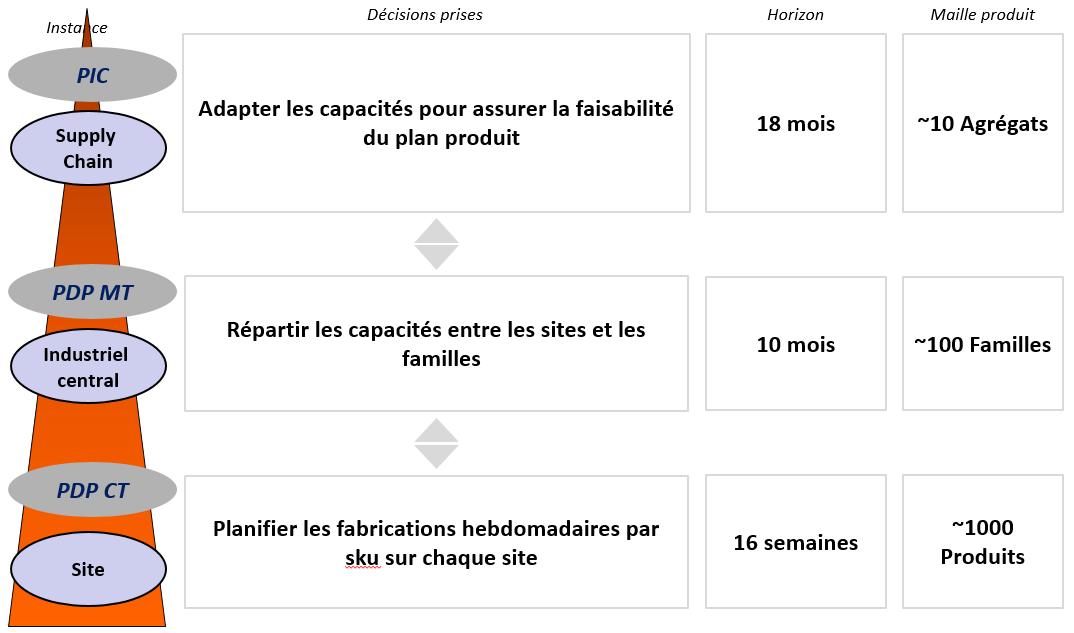
\includegraphics[width=\textwidth]{main/introduction/images/exemple_SC_luxe.png}
%   \caption{Exemple d'organisation de la Supply Chain d'un acteur du luxe}
%   \label{fig:exemple-SC-luxe}
% \end{figure}


% \section{Conséquences et problèmes étudiés}


% Optimsation multi-objectif : triangle coût / stock / service. (coût = coût hors stock).


% 2 sujets traités:
% \begin{itemize}
%   \item le niveau de multi-sourcing (moyen terme).
%   \begin{itemize}
%     \item Objectif : minimiser les coût de la création du multi-sourcing
%     \item Contrainte : taux de service client
%     \item Décisions : affectation produits / site
%   \end{itemize}
%   \item la plannification sous contrainte de flexibilité (court terme) décliné en deux axes :
%   \begin{itemize}
%     \item Optimization des paramètres des outils de PDP
%     \begin{itemize}
%       \item Objectif : minimiser le coût du stock
%       \item Contrainte : flexibilité industrielle (nombre de changements)
%       \item Décisions : Couverture de la production de chaque produits
%     \end{itemize}
%     \item Création du PDP en intégrant directement la contrainte de flexibilité
%     \begin{itemize}
%       \item Objectif : minimiser le coût du stock
%       \item Contrainte : flexibilité industrielle (nombre de changements)
%       \item Décisions : période de production et quantité produite pour chaque produit
%     \end{itemize}
%   \end{itemize}
% \end{itemize}


% Parler de la flexibilité du mix produit ! C'est ce qu'on optimise (ie : volume constant.)

\bookmarksetup{startatroot}
\addtocontents{toc}{\bigskip}

\cleardoublepage
\part{Continuous-time inventory models}
\label{part:continuous-review-inventory-model}
%!TEX root=../../thesis_ESG.tex
\chapter{Production on a single line}
\label{chap:lot-size:single-line}


\esgil{Vérifier la cohérence. \emph{Setup} désigne le lancement de la production (\ie un instant discret). \emph{Order of production} désigne le setup et la durée de production qui suit (\ie un intervalle).}


% \begin{itemize}
%   \item bibliographie
%   \item Flexibilité
%   \item Production on a single line
%   \item campagne de production ou batch de production
% \end{itemize}


As explained in \cref{sec:business-context:argon:pdp}, the objective is to reduce inventory.\vl{cumulated inventory}
This chapter presents a model whose aims at deciding the optimal cycle stocks.



\section{Motivations}
\label{sec:lot-size:single-line:motivations}

Cycle stocks form the portion of stocks\vl{inventory ?} that varies over time due to production and demand satisfaction.
Low cycle stocks contribute to globally decrease inventory but it requires a high flexibility of means of production.
At this level of decision,\vl{rappeler qu'on parle du niveau tactique} flexibility is fixed and industrial aims at deciding the values of cycle stocks of each item which minimize the global inventory.


Many production systems are managed using $(r,\lot)$ policies or similar ones.
This kind of policies defines for each item a level $r$ and a quantity $\lot$ such that: when inventory level of item reaches level $r$, a quantity $\lot$ is produced.
A common variation uses cover-sizes.
Quantity $\lot$ is replaced by a time $\cover$ called \emph{cover-size}.
When inventory level of item $i$ reaches level $r$, quantity produced is the cumulative demand of the $\cover$ next units of time.
Both are used by industrials (and are equivalent when demand does not depend on time).


\section{Deterministic settings}
\label{sec:lot-size:single-line:deterministic}

In this whole section, data are assumed to be deterministic.


\subsection{Problems}
\label{sec:lot-size:single-line:deterministic:problems}

The problem described by Argon Consulting considers an assembly line producing a set $\REF$ of items over an infinite horizon.
%The capacity needed (in time units) to produce one unit of item $i$ is $\rate_i$.
The internal production time of item $i$ (\ie the quantity of item $i$ produced in one time unit) is $\rate_i$.
Inventory $\inventory_i$ of item $i$ must satisfy demand, known in advance.
Thus, it continuously decreases by $\demand_i<\rate_i$ units per time unit when there is no production and continuously increases by $\rate_i-\demand_i$ units per time unit when item $i$ is produced.


%We call \emph{order of production} of an item $i$ an interval of time $[t_1,t_2]$ dedicated to the production of $i$ such that $t_1<t_2$ production starts at $t_1$ and stops at $t_2$.
We call \emph{order of production} of an item $i$ a pair $\bracket{t_i,\theta_i}$ such that production of item $i$ starts at $t$ and lasts $\theta_i$ units of time.
We call \emph{production setup} or simply \emph{setup} the beginning of an order of production.
Orders of production of item $i$ can be placed at any time, even simultaneously (like in~\cite{Ohno2001} where authors assume the immediate replenishment of the order with lead time).
However, the cover $\cover_i$ of a given item $i$ has to be the same over the infinite horizon.
By definition of the cover, a solution is entirely defined by a sequence $\bracket{t_i,\cover_i}_{i\in\REF}$ where $t_i$ is the first setup of item $i$ and $\cover_i>0$ is the cover of item $i$.
Indeed, we directly obtain the duration $\theta_i=\frac{\demand_i}{\rate_i}\cover_i$ and the start $t_i+k\cover_i$ ($k\in\ZZ_+$) of each order of production of item $i$.

Thus, for each item $i$, inventory $\inventory_i\bracket{t}$ is nonnegative and follows the dynamic
\begin{equation}\label{eq:lot-size:single-line:deterministic:motivations:dynamic}
  \dot{\inventory}_i\bracket{t} =
  \left\{
  \begin{array}{ll}
  \rate_i-\demand_i
  & \ds\mbox{if}\ t\in\bigcup_{k\in\ZZ_+} \left[t_i+k\cover_i,t_i+\bracket{k+\frac{\demand_i}{\rate_i}}\cover_i\right),
  \\
  -\demand_i
  & \mbox{otherwise}.
  \end{array}
  \right.
\end{equation}
\esgil{Ajouter figure en dans de scie avec un décalage vers le haut et un stock initial.}

%(It imposes that the solution is periodic for each item.)
The flexibility being modeled by a constraint and not by setup costs (see \cref{sec:business-context:argon:pdp}), in average over the infinite horizon, the number of setups per unit time for all items must be lower than $\nbsetups$ which can be written as
\begin{equation}\label{eq:lot-size:single-line:deterministic:motivations:flexibility}
  \limsup_{\horizon\rightarrow+\infty}\ \frac{1}{\horizon} \sum_{i\in\REF} \left\lfloor\frac{\horizon-t_i}{\cover_i}\right\rfloor \le \nbsetups.
\end{equation}


For each item $i$, there is an initial inventory $\inventory_i\bracket{0}\in\RR_+$ given in input.


Since inventory varies over times, the cycle stock is measured using its average value over an infinite horizon.
Storing one unit of item $i$ incurs a unit holding cost $\holding_i>0$ per unit time.
Objective is to find the covers which minimize the average cycle stock over infinite horizon
\begin{equation}
  \limsup_{\horizon\rightarrow+\infty}\ \frac{1}{\horizon} \sum_{i\in\REF} \holding_i \int_0^{\horizon}\inventory_i\bracket{t}dt
\end{equation}
while satisfying every constraints.\vl{cite constraint or write the whole problem}

% The problem can be written as
% \begin{subequations}\label{eq:lot-size:single-line:deterministic}
%   \begin{align}
%   \min\quad & \ds \lim_{\horizon\rightarrow+\infty} \frac{1}{\horizon} \sum_{i\in\REF} \holding_i \int_0^{\horizon}\inventory_i\bracket{t}dt
%   \label{eq:lot-size:single-line:deterministic:unconstrained}
%   \\
%   \st\quad  & \ds \lim_{\horizon\rightarrow+\infty} \frac{1}{\horizon} \sum_{i\in\REF} \left\lfloor\frac{\horizon-t_i}{\cover_i}\right\rfloor \le \nbsetups
%   \label{eq:lot-size:single-line:deterministic:unconstrained}
%   \\
%   & \dot{\inventory}_i\bracket{t} =
%   \left\{
%   \begin{array}{ll}
%   \rate_i-\demand_i & \ds\mbox{if}\ t\in\bigcup_{k\in\ZZ_+} \left[t_i+k\cover_i,t_i+\bracket{k+\frac{\demand_i}{\rate_i}}\cover_i\right)
%   \\
%   -\demand_i & \mbox{otherwise}
%   \end{array}
%   \right.
%   && \forall i\in\REF,\ \forall t\in\RR_+,
%   \\
%   & \inventory_i\bracket{t} \ge 0 && \forall i\in\REF,\ \forall t\in\RR_+,
%   \\
%   & t_i \ge 0 && \forall i\in\REF,
%   \\
%   & \cover_i > 0 && \forall i\in\REF.
%   \label{eq:lot-size:single-line:deterministic:unconstrained}
%   \end{align}
% \end{subequations}


\medskip


Since this model is a variation of the \emph{Economic Production Quantity model (EPQ)}, we call it \emph{Economic Production Quantity model with Bounded number of Setups (EPQ-BS)}.
We will consider two versions of this problem:
\begin{itemize}
  \item the covers can be any nonnegative real numbers,
  \item the covers have to be inverses of integers.
\end{itemize}
In other words, since a cover is a time period, the production frequencies are unconstrained in the first version, while there are constrained to be integers in the second one.
We qualify the first version of being {\em unconstrained} and the second of being {\em integer}.


Integer version relies on practical reasons.
For decision makers, it is sometimes easier to use frequencies and thus to know that an item is produced once a month, twice a month, etc.



\subsection{Bibliography}

\textbf{literature review}

\begin{itemize}
   \item \cite{Gayon2016} Continuous-review inventory models for single item
\end{itemize} 

Multi-item

\begin{itemize}
  \item \cite{Hadley1963} first to note that perhaps the most important real world constraints are budget restrictions on the amount that can be invested in inventory.
  \item \cite{Schrady1971} Minimization of total time-weighted shortage subject to inventory investment (holding cost) and to reorder workload.
  They use our formula to find a solution but does not prove it optimality.
  \item \cite{Daeschner1975} Model with limited number of reorder transactions to be considered in the present allocation.
  \item \cite{Ohno2001} Minimization of the holding cost, backorder cost and ordering cost subject to capacity constraints on the inventory.
\end{itemize}


\medskip

\textbf{Ordering}

\begin{itemize}
  \item \cite{Harris1913} Economic Order Quantity (in French: ``Formule de Wilson'' because it was extensively used by R. H. Wilson from 1934)
  \begin{itemize}
    \item single item
    \item cost structure: proportional holding cost, variable and fixed order cost
    \item stationary demand $\demand$
    \item average cost over infinite horizon
  \end{itemize}
  \item Time varying demand $\demand(t)$
  \begin{itemize}
    \item \cite{Resh1976,Donaldson1977} $\demand(t)=\alpha t+\gamma$ polynomial
    \item \cite{Barbosa1978} $\demand(t)=\alpha t^{\beta}$
    \item difficult in general
  \end{itemize}
\end{itemize}

Classical policy: Zero Inventory Ordering policy $(r,q)$ (Order quantity $q$ when current inventory is $r$)

\medskip

\textbf{Production}

\begin{itemize}
  \item Economic Production Quantity (extension of EOQ with limited production capacity) \cite{Taft1918}
  \begin{itemize}
    \item Limited production capacity
  \end{itemize}
\end{itemize}


\medskip

\esgil{complete bibliography}



\subsection{Unconstrained EPQ-BS}
\label{sec:lot-size:single-line:models:unconstrained}


%Using the average value of the inventory of each product over time, the optimization problem can be written as follow:
We address the following alternative mathematical problem.
%We claim that the following optimization problem is a correct model of the unconstrained EPQ-BS in its unconstrained version:
\begin{subequations}\label{eq:lot-size:single-line:deterministic:unconstrained}
  \begin{align}
  \min\quad & \ds\sum_{i\in\REF} \frac{1}{2}\holding_i\tilde{\demand}_i\cover_i
  \label{eq:lot-size:single-line:deterministic:unconstrained:objective}
  \\
  \st\quad  & \ds\sum_{i\in\REF} \frac{1}{\cover_i} \le \nbsetups
  \label{eq:lot-size:single-line:deterministic:unconstrained:flexibility}
  \\
       & \cover_i > 0 && \forall i\in\REF,
  \label{eq:lot-size:single-line:deterministic:unconstrained:positivity}
  \end{align}
\end{subequations}
where $\tilde{\demand}_i=\bracket{1-\frac{\demand_i}{\rate_i}}\demand_i$.
% is the reduced value of the demand.

\begin{thm}\label{thm:lot-size:single-line:deterministic:unconstrained:optimality}
Problem~\eqref{eq:lot-size:single-line:deterministic:unconstrained} has a unique optimal solution $(\cover_i^*)_{i\in\REF}$ with
\begin{equation}
  \cover_i^*= \frac{\sum_{j\in\REF}\sqrt{\holding_j\tilde{\demand}_j}}{\nbsetups\sqrt{\holding_i\tilde{\demand}_i}}\qquad\forall i\in\REF
\end{equation}
and optimal cost equal to $\frac{1}{2\nbsetups}\bracket{\sum_{i\in\REF}\sqrt{\holding_i\tilde{\demand_i}}}^2$.

Moreover, the optimal solution of Problem~\eqref{eq:lot-size:single-line:deterministic:unconstrained} is the optimal solution of unconstrained EPQ-BS.
\end{thm}


Formulation \eqref{eq:lot-size:single-line:deterministic:unconstrained} have many advantages.
First, it is much simpler than the original formulation of \cref{sec:lot-size:single-line:deterministic:problems}.
Second, it removes from the formulation the first setups of production $\bracket{t_i}_i$ which are not a desired output.


The correctness\vl{unclear: the link between both problem} is however not necessarily immediate.
As we will see, formulation \eqref{eq:lot-size:single-line:deterministic:unconstrained} assumes that optimal policy is \emph{Zero-Inventory-Ordering (ZIO)}.
We recall that a policy is said to be ZIO if an order can only occurs when the inventory is zero.
Due to flexibility constraint \eqref{eq:lot-size:single-line:deterministic:motivations:flexibility}, production should have to be anticipated before inventory reach zero.


% For each item $i$, let $\freq_i\bracket{t}$ be the number of setups during the interval $[0,t)$ and $\freq_i$ the average number of setups per time unit over the infinite horizon.
% Let $t_i$ be the first production setup of item $i$.
% Then, according to problem description in \cref{sec:lot-size:single-line:deterministic:problems}, production setups occur at times $t_i+k\,\cover_i$ with $k\in\ZZ_+$.


\begin{lem}\label{lem:lot-size:single-line:deterministic:unconstrained:optimality}
Problem~\eqref{eq:lot-size:single-line:deterministic:unconstrained} has a unique optimal solution $(\cover_i^*)_{i\in\REF}$.
\end{lem}


\begin{proof}
Since Problem~\eqref{eq:lot-size:single-line:deterministic:unconstrained} is a convex problem, solving it is straightforward using the Karush-Kuhn-Tucker conditions which gives the unique solution
\begin{equation}
  \cover_i^*= \frac{\sum_{j\in\REF}\sqrt{\holding_j\tilde{\demand}_j}}{\nbsetups\sqrt{\holding_i\tilde{\demand}_i}}\qquad\forall i\in\REF,
\end{equation}
with optimal cost $\frac{1}{2\nbsetups}\bracket{\sum_{i\in\REF}\sqrt{\holding_i\tilde{\demand_i}}}^2$.
\end{proof}



\begin{lem}\label{lem:lot-size:single-line:models:average-setup}
%For each item $i$, average number $\freq_i$ of setups per time unit over the infinite horizon is equal to $\frac{1}{\cover_i}$ where $\cover_i$ is the cover and flexibility constraint described in \cref{sec:lot-size:single-line:deterministic:problems} can be written as
Flexibility constraint \eqref{eq:lot-size:single-line:deterministic:motivations:flexibility} is equivalent to
$\ds\sum_{i\in\REF} \frac{1}{\cover_i} \le \nbsetups$.
\end{lem}


\begin{proof}
For a time $\horizon>t_i$, the average number of setups per time unit during the interval $[0,\horizon)$ is
$\frac{1}{\horizon}\left\lfloor\frac{\horizon-t_i}{\cover_i}\right\rfloor$
which converges to $\frac{1}{\cover_i}$ when $\horizon$ goes to infinity.
Equivalence immediately follows.
\end{proof}


Note that this formulation is independent of the first production setup $t_i$.
Then, choice of $t_i$ is only constrained by positive inventory.


\begin{lem}\label{lem:lot-size:single-line:models:ZIO}
Let $\bracket{t_i^*,\cover_i^*}_{i\in\REF}$ be an optimal solution of unconstrained EPQ-BS.
Then, this solution is Zero-Inventory-Ordering, and its cost is given by
\begin{equation}
  \sum_{i\in\REF}\frac{1}{2}\holding_i\bracket{1-\frac{\demand_i}{\rate_i}}\demand_i\cover_i^*
\end{equation}
and we have $t_i^*=\frac{\inventory_i(0)}{\demand_i}$ for each item $i$.
\end{lem}


\begin{proof}
Let $\bracket{t_i^*,\cover_i^*}_{i\in\REF}$ be an optimal solution of unconstrained EPQ-BS.
Using the dynamic \eqref{eq:lot-size:single-line:deterministic:motivations:dynamic}, we have for each item $i$
\begin{equation}
  S_{i,0}
  =
  \int_0^{t_i^*}\inventory_i\bracket{t}dt
  = \frac{1}{2}\bracket{2\inventory_i\bracket{0}-t_i^*\demand_i}t_i^*,
\end{equation}
and for each $k\in\ZZ_+$
\begin{equation}
  S_{i,k}
  =
  \int_{t_i^*+k\cover_i^*}^{t_i^*+\bracket{k+1}\cover_i^*}\inventory_i(t)dt
  =
  \bracket{\inventory_i(0)-\demand_i t_i^*}\cover_i^*
  + \frac{1}{2}\bracket{1-\frac{\demand_i}{\rate_i}}\demand_i\cover_i^{*2}.
\end{equation}
Let $\horizon$ be a real number greater than $t_i^*$.
Splitting the integral, we get
\begin{equation}
  \frac{1}{\horizon} S_{i,0}
  + \frac{1}{\horizon} \sum_{k=1}^{\left\lfloor\frac{\horizon-t_i^*}{\cover_i^*}\right\rfloor-1} S_{i,k}
  \le
  \frac{1}{\horizon} \int_0^{\horizon}\inventory_i\bracket{t}dt
  \le
  \frac{1}{\horizon} S_{i,0}
  + \frac{1}{\horizon} \sum_{k=1}^{\left\lfloor\frac{\horizon-t_i^*}{\cover_i^*}\right\rfloor} S_{i,k}
\end{equation}
and the average cycle stock on infinite horizon for item $i$ follows:
\begin{equation}
  \lim_{\horizon\rightarrow\infty} \frac{1}{\horizon} \int_0^{\horizon}\inventory_i\bracket{t}dt
  =
  \inventory_i(0)-\demand_i t_i^*
  + \frac{1}{2}\bracket{1-\frac{\demand_i}{\rate_i}}\demand_i\cover_i^*.
\end{equation}
Thanks to \cref{lem:lot-size:single-line:models:average-setup}, $\bracket{t_i^*,\cover_i^*}_{i\in\REF}$ is feasible for every $t_i^*\ge\frac{\inventory_i(0)}{\demand_i}$ but optimality implies that $t_i^*=\frac{\inventory_i(0)}{\demand_i}$.
Then, an optimal solution of unconstrained EPQ-BS is Zero-Inventory-Ordering and its cost is
\begin{equation}
  \sum_{i\in\REF}\frac{1}{2}\holding_i\bracket{1-\frac{\demand_i}{\rate_i}}\demand_i\cover_i^*.
\end{equation}
\end{proof}


%Thanks to \cref{prop:lot-size:single-line:models:average-setup} and \cref{prop:lot-size:single-line:models:ZIO}, problem \eqref{eq:lot-size:single-line:deterministic:unconstrained} is a correctly models the unconstrained version of the problem described \cref{sec:lot-size:single-line:deterministic:problems}.



\begin{proof}[Proof of \cref{thm:lot-size:single-line:deterministic:unconstrained:optimality}]
\cref{lem:lot-size:single-line:models:average-setup} and \cref{lem:lot-size:single-line:models:ZIO} prove that every optimal solutions of unconstrained EPQ-BS is a solution of Problem \ref{eq:lot-size:single-line:deterministic:unconstrained} with the same cost.
Conversely, an optimal solution of Problem \ref{eq:lot-size:single-line:deterministic:unconstrained} can be completed in a solution of unconstrained EPQ-BS with the same cost setting the first production setup $t_i$ of item $i$ equal to $\frac{\inventory_i(0)}{\demand_i}$.
Then, the unique optimal solutions of Problem \ref{eq:lot-size:single-line:deterministic:unconstrained} (\cref{lem:lot-size:single-line:deterministic:unconstrained:optimality}) is the optimal solution of unconstrained EPQ-BS.
\end{proof}


\medskip


Note that model simply adapts to case where production is considered instantaneous (\ie $\rate_i\rightarrow\infty$).
In this case, just use real demand $\demand_i$ instead of reduced demand $\bar{\demand}_i=\bracket{1-\frac{\demand_i}{\rate_i}}\demand_i$.


% Then, if such a limit exists, we must have
% \begin{equation}
%   \limsup_{t\rightarrow\infty}\frac{1}{t} \sum_{i\in\REF}\freq_i\bracket{t}\le\nbsetups.
% \end{equation}


% \begin{proof}
% Scheme of proof:
% \begin{itemize}
%   \item expression of the constraint
%   \item ZIO policy
%   \item expression of the objective
% \end{itemize}
% \end{proof}




% Using the production frequencies $\freq_i=\frac{1}{\cover_i}$ of product $r$, we get the optimal frequencies:
% \begin{equation}
%   \freq_i^* = \frac{1}{\cover_i^*}
%             = \frac{\nbsetups\sqrt{\holding_i\demand_i}}{\sum_{s\in\REF}\sqrt{\holding_s\demand_s}}
%             \quad \forall i\in\REF,
% \end{equation}
% and the associated holding cost is $\frac{1}{2\nbsetups}\bracket{\sum_{i\in\REF}\sqrt{\holding_i\demand_i}}^2$.


% \esgil{Write the proof}



\subsection{Integer EPQ-BS}


%In some cases, it is easier for industrial to use integer frequencies.
As explained in \cref{sec:lot-size:single-line:models:unconstrained}, dealing with finite or infinite internal production time $\rate_i$ is very similar since, it is sufficient to use the demand $\demand_i$ or the reduced demand $\tilde{\demand}_i$ in problem \eqref{eq:lot-size:single-line:deterministic:unconstrained}.
Thus, we only write the case with infinite internal production time $\rate_i$.
\begin{subequations}\label{eq:lot-size:single-line:deterministic:integer}
  \begin{align}
  \min\quad & \ds\sum_{i\in\REF} \frac{1}{2}\holding_i\demand_i\frac{1}{\freq_i}
  \label{eq:lot-size:single-line:deterministic:integer:objective}
  \\
  \st\quad  & \ds\sum_{i\in\REF} \freq_i \le \nbsetups
  \label{eq:lot-size:single-line:deterministic:integer:flexibility}
  \\
       & \freq_i \in \ZZ_+^* && \forall i\in\REF,
  \label{eq:lot-size:single-line:deterministic:integer:positivity}
  \end{align}
\end{subequations}
where $\freq_i=\frac{1}{\cover_i}$ is the average number of setups per time unit over the infinite horizon.


Proving that optimal solutions of Problem \eqref{eq:lot-size:single-line:deterministic:integer} are the optimal solution of integer EOQ-BS is very similar to the unconstrained case.


\medskip


This formulation is a special case of the integer simple resource allocation problem:
\begin{equation}
  \max\crbracket{\sum_{i\in\REF} f_i\bracket{\freq_i} \Big| \sum_{i\in\REF}\freq_i=\nbsetups,\quad\freq\in \ZZ_+^*}
\end{equation}
where the $f_i$ are concave.
\esgil{Check the definition of the problem}

The fastest algorithm known has a $O\bracket{\card{\REF}\log{\frac{\nbsetups}{\card{\REF}}}}$ running time and was proposed by \cite{Frederickson1982} and then simplified by \cite{Hochbaum1994}.
Implementation of these algorithms is not easy.
Dynamic programming might be used instead, but its complexity is only $O\bracket{\card{\REF}\nbsetups^2}$ which is pseudo-polynomial.



\section{Stochastic settings}


\subsection{Problem}
\label{sec:lot-size:single-line:stochastic:problem}


As in \cref{sec:lot-size:single-line:deterministic:problems}, cycle stocks are managed using $(r,\cover)$ policies (\ie cover policies).
However, in real life, many parameters are not known in advance.
An obvious example is demand which can changes due to forecast errors, marketing promotions, passing fads.
Randomness can also comes from production means.
Failures, holidays or strikes can affect internal production time.


Production means are assumed to be reliable and we only consider randomness on demand.
The problem becomes an assembly line still producing a set $\REF$ of items over an infinite horizon.
The internal production time of item $i$ is $\rate_i$.
Inventory $\va\inventory_i$ of item $i$ must satisfy a random demand.
Then it continuously decreases by $\va\demand_i<\rate_i$ units per time unit when there is no production and continuously increases by $\rate_i-\va\demand_i$ units per time unit when item $i$ is produced.
%Note that inventory $\va\inventory_i$ and demand $\va\demand_i$ are in bold to indicate that they are random.
Moreover, $\va\demand_i$ is assumed to be almost surely lower than $\rate_i$.


Orders of production of item $i$ can be placed at any time, even simultaneously but the cover $\cover_i$ of a given item $i$ has to be the same over the infinite horizon.
Covers are decided before the demand is revealed.
When demand is revealed once and for all, the duration $\theta_i$ of the order of production is fixed at value $\frac{\demand_i}{\rate_i}\cover_i$.
Covers $\bracket{\cover_i}_i$ are called \emph{first-stage decision} since they are decided before hazard realization whereas first setups $\bracket{\va t_i}_i$ and durations $\bracket{\va\theta_i}_i$ are called second-stage decisions.\vl{(or recourse).}

Thus, for each item $i$, inventory $\va\inventory_i\bracket{t}$ is nonnegative and follows almost surely the dynamic
\begin{equation}\label{eq:lot-size:single-line:deterministic:motivations:dynamic}
  \dot{\va\inventory}_i\bracket{t} =
  \left\{
  \begin{array}{ll}
  \rate_i-\va\demand_i
  & \ds\mbox{if}\ t\in\bigcup_{k\in\ZZ_+} \left[t_i+k\cover_i,t_i+\bracket{k+\frac{\va\demand_i}{\rate_i}}\cover_i\right),
  \\
  -\va\demand_i
  & \mbox{otherwise}.
  \end{array}
  \right.
\end{equation}

%(It imposes that the solution is periodic for each item.)
Flexibility is still modeled by a constraint.
In average over the infinite horizon, the number of setups per unit time for all items must be lower than $\nbsetups$ which can be written as
\begin{equation}
  \limsup_{\horizon\rightarrow+\infty}\ \frac{1}{\horizon} \sum_{i\in\REF} \left\lfloor\frac{\horizon-t_i}{\cover_i}\right\rfloor \le \nbsetups.
\end{equation}

For each item $i$, there is an initial inventory $s_i\bracket{0}\in\RR_+$.


Storing one unit of item $i$ incurs a unit holding cost $\holding_i>0$ per unit time.
Objective is to find the covers which minimize the average cycle stock over infinite horizon
\begin{equation}
  \limsup_{\horizon\rightarrow+\infty}
  \ 
  \espe\sqbracket{
  \frac{1}{\horizon} \sum_{i\in\REF} \holding_i \int_0^{\horizon}\va\inventory_i\bracket{t}dt
  }
\end{equation}
while satisfying every constraints.


We call this problem \emph{stochastic Economic Production Quantity model with Bounded number of Setups (stochastic EPQ-BS)} and will consider the same two versions as in deterministic case:
\begin{itemize}
  \item the covers can be any nonnegative real numbers (called \emph{unconstrained}),
  \item the covers have to be inverses of integers (called \emph{integer}).
\end{itemize}



\subsection{Bibliography}

Source of randomness:
\begin{itemize}
  \item customer demand
  \item manufacturing time (internal production time)
  \item delivery lead time
\end{itemize}

Randomness was handled by probability (most cases) but also with fuzzy set theory (\eg \cite{Park1987,Lee1999,Wang2007} for extensions of the EOQ and \cite{Ziukov2015} for a complete review of the extensions of EOP, EPQ, Joint Economic Lot Sizing models).
In what follows, we focus on randomness represented by probability.

Literature often include backorder costs!

\medskip

\textbf{Ordering}

One period:
\begin{itemize}
  \item News-vendor problem \cite{Edgeworth88,Arrow1951}
\end{itemize}

Continuous-review:
\begin{itemize}
  \item adaptation of (r,q) policies with EOQ taking into account random demand during lead-time \cite{Gallego1998}
\end{itemize}

\medskip

\textbf{Production}




\esgil{Complete bibliography}



\subsection{Model}


%We claim that the following optimization problem is a correct model of the problem described in \cref{sec:lot-size:single-line:stochastic:motivations}.
We address the following alternative mathematical problem.
\begin{subequations}\label{eq:lot-size:single-line:stochastic:unconstrained}
  \begin{align}
  \min\quad & \ds\sum_{i\in\REF} \frac{1}{2}\holding_i\tilde{\tilde{\demand}}_i\cover_i
  \label{eq:lot-size:single-line:stochastic:unconstrained:objective}
  \\
  \st\quad  & \ds\sum_{i\in\REF} \frac{1}{\cover_i} \le \nbsetups
  \label{eq:lot-size:single-line:stochastic:unconstrained:flexibility}
  \\
       & \cover_i > 0 && \forall i\in\REF,
  \label{eq:lot-size:single-line:stochastic:unconstrained:positivity}
  \end{align}
\end{subequations}
where $\tilde{\tilde{\demand}}_i=\bracket{1-\frac{\espe\sqbracket{\va\demand_i}}{\rate_i}}\espe\sqbracket{\va\demand_i} - \frac{\vari\sqbracket{\va\demand_i}}{\rate_i}$.
%is the reduced value of the demand in stochastic case.

\begin{thm}\label{thm:lot-size:single-line:stochastic:unconstrained:optimality}
Problem~\eqref{eq:lot-size:single-line:stochastic:unconstrained} has a unique optimal solution $(\cover_i^*)_{i\in\REF}$ with
\begin{equation}
  \cover_i^*= \frac{\sum_{j\in\REF}\sqrt{\holding_j\tilde{\tilde{\demand}}_j}}{\nbsetups\sqrt{\holding_i\tilde{\tilde{\demand}}_i}}\qquad\forall i\in\REF
\end{equation}
and optimal cost equal to $\frac{1}{2\nbsetups}\bracket{\sum_{i\in\REF}\sqrt{\holding_i\tilde{\tilde{\demand}}_i}}^2$.

Moreover, the optimal solution of Problem~\eqref{eq:lot-size:single-line:stochastic:unconstrained} is the optimal solution of unconstrained stochastic EPQ-BS.
\end{thm}


Assuming that this formulation is correct\vl{?}, adaptation of results from deterministic cases (unconstrained and integer frequencies) to stochastic cases is straightforward.
Moreover, when the only randomness comes from the demand, we also show that the optimal solution is completely determined by the expectation and the variance of each of the demand $\va\demand_i$.

\vlil{faire une remarque sur le fait que ce n'est pas la solution donnée en remplacant $d_i$ par son espérance.}


\esgil{Complete the correctness of the model.}



\section{Numerical experiments}

\begin{itemize}
  \item Numerical experiments
  \item Lien avec la formule de Wilson
\end{itemize}


\subsection{Concluding remarks}



% A natural extension takes into account the internal production time $\internal_i$ which is the time needed to produce one unit of product $r$. In this case, the production is not instantaneous and during the production phase of $r$, the increase of the inventory is $\frac{1}{\internal_i}-\demand_i$ per time unit. Thus, the average value of the inventory of product $r$ is equal to $\frac{1}{2}\holding_i\demand_i\bracket{1-\internal_i\demand_i}$. Setting $\holding_i'=\holding_i\bracket{1-\internal_i\demand_i}$, we get the optimal frequencies:
% \begin{equation}
%   \freq_i^* = \frac{1}{\cover_i^*}
%             = \frac{\nbsetups\sqrt{\holding_i\demand_i\bracket{1-\internal_i\demand_i}}}{\sum_{s\in\REF}\sqrt{\holding_s\demand_s\bracket{1-\internal_s\demand_s}}}
%             \quad \forall i\in\REF,
% \end{equation}
% and the associated holding cost is $\frac{1}{2\nbsetups}\bracket{\sum_{i\in\REF}\sqrt{\holding_i\demand_i\bracket{1-\internal_i\demand_i}}}^2$.


\chapter{Production on several lines}
\label{chap:lot-size:several-lines}



\cref{chap:lot-size:single-line} was about to decide the optimal cycle stocks when only a single line is involved.
In this chapter, several are involved in production and we aim at deciding the part of demand assigned to each line and the cycle stocks for each each item on each line.



\section{Motivations}
\label{sec:lot-size:several-lines:motivations}


Context is almost the same than in \cref{chap:lot-size:single-line}.
A company aims at reducing it cycle stocks (which globally helps to decrease the inventory) subject to flexibility constraint of the assemblies lines.
In many applications, a company has many assembly lines and production of a single item may be done on several lines.
This kind of configuration is very common and are the consequences of multi-sourcing decisions previously made (see \cref{sec:business-context:argon:multi-sourcing} for a description of multi-sourcing issues).
These lines might be the same plants as well in different ones.
But, in both cases, it enables to increase flexibility of production and the workload between lines.


As in single line case, assembly lines are managed using $(r,\lot)$ policies or similar ones (like policies using cover).
The challenge of the multi-line case is that companies must decide the part of demand assigned to each line and the lot (or cover) used for the production of each item on each line.


In this chapter, we show how to compute the assignment of demand to lines and the lot-sizes and cover-sizes minimizing inventory subject to flexibility constraint.


\section{Problem}


The problem described by Argon Consulting considers a set $\lines$ of assembly lines producing a set $\REF$ of items over an infinite horizon.
Each line is managed using the same policy than in \cref{chap:lot-size:single-line}.
Parameters for each line $\ell$ are then the same (with an index depending on the line) and we recall them for the sake of completeness.
The internal production time of item $i$ on line $\ell$ (\ie the quantity of item $i$ produced in one time unit) is $\rate_i^{\ell}$.
Inventory $\inventory_i^\ell$ of item $i$ must satisfy demand, known in advance.
The part of demand for item $i$ assigned to line $\ell$ is modeled by a continuous decrease $\demand_i^{\ell}<\rate_i^{\ell}$ units per time unit when line $\ell$ does not produce item $i$ and a continuous increase $\rate_i^{\ell}-\demand_i^{\ell}$ units per time unit when item $i$ is produced.
The whole demand or item $i$ is modeled by a continuous decrease $\demand_i$ which is assumed positive.
Since the whole demand must satisfied, we have
\begin{equation}\label{eq:lot-size:multi-line:motivations:whole-demand}
  \sum_{\ell\in\lines}\demand_i^{\ell}=\demand_i\qquad\forall i\in\REF.
\end{equation}


If item $i$ is assigned to line $\ell$, the first time it is produced on line $\ell$ is $t_i^{\ell}$.
and the production is launched for every $t_i^{\ell}+k\cover_i^{\ell}$ where $k\in\ZZ_+$ and $\cover_i^{\ell}$ is the cover-size of item $i$ for the line $\ell$.
Each production on line $\ell$ lasts $\frac{\demand_i^{\ell}}{\rate_i^{\ell}}\cover_i^{\ell}$ in order to produce exactly the demand assign to line $\ell$ for the next $\cover_i^{\ell}$ unit of time.
(Each of these quantities is not defined if item $i$ is not assigned to line $\ell$.)
Like single-line case, the productions of several items can be placed simultaneously.


Thus, if item $i$ is assigned to line $\ell$, inventory $\inventory_i^{\ell}\bracket{t}$ generated par line $\ell$ is continuous, right and left differentiable, nonnegative and follows the dynamic
\begin{equation}\label{eq:lot-size:multi-line:motivations:dynamic}
  \dot{\inventory}_i^{\ell}\bracket{t} =
  \left\{
  \begin{array}{ll}
  \rate_i^{\ell}-\demand_i^{\ell}
  & \ds\mbox{if}\ t\in\bigcup_{k\in\ZZ_+} \left[t_i^{\ell}+k\cover_i^{\ell},t_i^{\ell}+\bracket{k+\frac{\demand_i^{\ell}}{\rate_i^{\ell}}}\cover_i^{\ell}\right),
  \\
  -\demand_i^{\ell}
  & \mbox{otherwise}.
  \end{array}
  \right.
\end{equation}


Contrary to single-line case, each line has a limited capacity.
In average over the infinite horizon, the percentage of time spend for production of all items assigned to line $\ell$ must be lower than $\capacity^{\ell}<1$ which can be written as
\begin{equation}\label{eq:lot-size:multi-line:motivations:capacity}
  \sum_{i\in\REF}\frac{\demand_i^{\ell}}{\rate_i^{\ell}}\le\capacity^{\ell}\qquad\forall \ell\in\lines.
\end{equation}
Indeed, each production of item $i$ on line $\ell$ lasts $\frac{\demand_i^{\ell}}{\rate_i^{\ell}}\cover_i^{\ell}$ (in order to produce exactly the demand for the next $\cover_i$ unit of time) and then uses $\frac{\demand_i^{\ell}}{\rate_i^{\ell}}$ percents of the production time.


Like single-line case, in average over the infinite horizon, the number of setups per unit time for all items must be lower than $\nbsetups^{\ell}$ which can be written as
\begin{equation}\label{eq:lot-size:multi-line:motivations:flexibility}
  \limsup_{\horizon\rightarrow+\infty}\ \frac{1}{\horizon} \sum_{i\in\REF^{\ell}} \left\lfloor\frac{\horizon-t_i^{\ell}}{\cover_i^{\ell}}\right\rfloor \le \nbsetups
\end{equation}
where $\REF^{\ell}$ is the set of items produced by line $\ell$.


For each item $i$, there is an initial inventory $\inventory_i\bracket{0}\in\RR_+$ given in input.


Storing one unit of item $i$ produced by line $\ell$ incurs a unit holding cost $\holding_i^{\ell}>0$ per unit time.
The objective is to find the part of demand $\demand_i^{\ell}$ for item $i$ assigned to line $\ell$ and the cover-sizes $\cover_i^{\ell}$ which minimize the average cycle stock of every lines over infinite horizon
\begin{equation}
  \limsup_{\horizon\rightarrow+\infty}\ \frac{1}{\horizon} \sum_{\ell\in\REF} \sum_{i\in\REF} \holding_i \int_0^{\horizon}\inventory_i^{\ell}\bracket{t}dt
\end{equation}
while satisfying nonnegative inventory, constraints~\eqref{eq:lot-size:multi-line:motivations:whole-demand} to \eqref{eq:lot-size:multi-line:motivations:flexibility}.

\medskip


We call this model the \emph{multi-line Economic Production Quantity model with Bounded number of Setups (multi-line EPQ-BS)}.

Like for single line case, when using lot-sizes $\lot_i^{\ell}$ instead of cover-sizes, the multi-line EPQ-BS can be simply adapt using $\lot_i^{\ell}=\demand_i^{\ell}\cover_i^{\ell}$.



\section{Bibliography}

\begin{itemize}
  \item bibliographie (groupée avec celle du chapitre single line?)
  \item Flexibilité
  \item Production on a several lines
\end{itemize}


Single item multi-line one retailer\\
Production allocation and shipment policies in a multiple-manufacturer–single-retailer supply chain
S. S. Park , T. Kim \& Y. Hong 


Single item multi-line one retailer With procurement (+ NP-complete)\\
T. Kim, Y. Hong * and J. Lee, Joint economic production allocation and ordering policies in a supply chain consisting of multiple plants and a single retailer, International Journal of Production Research, 43, 17, (3619), (2005).


A multi-machine multi-product EPQ problem for an imperfect manufacturing system considering utilization and allocation decisions
Author links open overlay panelAmir HosseinNobilaAmir Hosein AfsharSedighaLeopoldo EduardoCárdenas-Barrón
2016
=> One item by machine (1st level). Then decide cycle length.
minimizes total cost of the inventory system, including utilization, setup, production, holding and disposal cost


\section{Solving the multi-line EPQ-BS}


\esgil{Missing: $\NP$-hardness of the model?}



%Using the average value of the inventory of each product over time, the optimization problem can be written as follow:
We address the following alternative mathematical problem.
%We claim that the following optimization problem is a correct model of the unconstrained EPQ-BS in its unconstrained version:
\begin{subequations}\label{eq:lot-size:multi-line:unconstrained}
  \begin{align+}
  \min\quad & \ds\sum_{i\in\REF} \frac{1}{2\nbsetups^{\ell}}\bracket{\sum_{i\in\REF}\sqrt{\holding_i^{\ell}\bracket{1-\frac{\demand_i^{\ell}}{\rate_i^{\ell}}}\demand_i^{\ell}}}^2
  \label{eq:lot-size:multi-line:unconstrained:objective}
  \\
  \st\quad  & \sum_{\ell\in\lines}\demand_i^{\ell}=\demand_i && \forall i\in\REF,
  \label{eq:lot-size:multi-line:unconstrained:flexibility}
  \\
            & \sum_{i\in\REF}\frac{\demand_i^{\ell}}{\rate_i^{\ell}}\le\capacity^{\ell} && \forall \ell\in\lines,
  \label{eq:lot-size:multi-line:unconstrained:capacity}
  \\
            & \demand_i^{\ell} \ge 0 && \forall i\in\REF.
  \label{eq:lot-size:multi-line:unconstrained:positivity}
  \end{align+}
\end{subequations}


\begin{thm}\label{thm:lot-size:multi-line:unconstrained:optimality}
Optimal solutions of Problem~\eqref{eq:lot-size:multi-line:unconstrained} can be found on the extreme point of the constraints polyhedron using an algorithm minimizing concave function on a polyhedron.

Moreover, an optimal solution $\bracket{\demand_i^{\ell*}}_{i\in\REF,\ell\in\lines}$ of Problem~\eqref{eq:lot-size:multi-line:unconstrained} can be completed in an optimal solution of multi-line EPQ-BS setting for each item $i$ assigned to line $\ell$
\begin{equation}\label{eq:lot-size:multi-line:unconstrained:optimal-cover}
  \cover_i^{\ell*}= \frac{\sum_{j\in\REF}\sqrt{\holding_j\bracket{1-\frac{\demand_i^{\ell*}}{\rate_i}}\demand_i^{\ell*}}}{\nbsetups\sqrt{\holding_i\bracket{1-\frac{\demand_i^{\ell*}}{\rate_i}}\demand_i^{\ell*}}}.
\end{equation}
\end{thm}


Minimization of concave function over a polyhedron is $\NP$-hard since it contains Zero-One Integer Programming (see \cite{Raghavachari1969}) which is known to be $\NP$-hard (see \cite{Garey1979}).
However, there are many algorithms to solve this kind of problem (see \cite{Tuy1964} for the first proposed algorithm and \cite{Benson1998} for a review) and it is well know that an optimal solution can be found in an extreme point of the constraints polyhedron (see \cite{Benson1985}).


Note that \cref{eq:lot-size:multi-line:unconstrained:optimal-cover} is well-defined.
Indeed, $\capacity^{\ell}$ is lower than 1.
Thus, constraint~\eqref{eq:lot-size:multi-line:unconstrained:capacity} and definition of the cover-sizes only for the items assigned to a line ensure that $\bracket{1-\frac{\demand_i^{\ell*}}{\rate_i}}\demand_i^{\ell*}>0$.


We recall the concave monotone superposition of a convex vector-function by a monotone convex function.


\begin{lem}[``Concave monotone superposition'']\label{lem:concave-monotone-superposition}
Let $C$ be a convex subset of $\RR^n$.
Let $f:x\in C \mapsto f(x) = \bracket{f_1(x),\ldots,f_k(x)}$ be vector-function on $C\subseteq\RR^n$ with concave components $f_i$, and assume that $F$ is a concave function on $\RR^k$ which is monotone, \ie such that $z\le z'$ implies that $F(z)\le F(z')$.
Then the superposition $\phi(x) = F\bracket{f(x)}=F\bracket{f_1(x),\ldots,f_k(x)}$ is concave on $C$.
\end{lem}


\begin{proof}
Let $x$ and $x'$ be two vectors of $C$ and let $\lambda$ be a real number in $(0,1)$.
Since each $f_i$ is concave, we have
$f\bracket{\lambda x +(1-\lambda) x'} \ge \lambda f(x) + (1-\lambda) f(x')$.
And then,
\begin{subequations}
\begin{align}
  F\bracket{f\bracket{\lambda x +(1-\lambda) x'}}
  &\ge F\bracket{\lambda f(x) + (1-\lambda) f(x')}
  && \mbox{(monotonicity of $F$)}
  \\
  &\ge \lambda F\bracket{f(x)} + (1-\lambda) F\bracket{f(x')}.
  && \mbox{(concavity of $F$)}
\end{align}
\end{subequations}
Finally $\phi\bracket{\lambda x +(1-\lambda) x'} \ge \lambda \phi(x) + (1-\lambda) \phi(x')$ and $\phi$ is concave on $C$.
\end{proof}



\begin{lem}\label{lem:concave-objective-function}
The objective function
\begin{equation}
\begin{array}{rccl}
  g: & \ds\bigcup_{\ell\in\lines}\bigcup_{i\in\REF} \sqbracket{0,\rate_i^{\ell}} & \to & \RR_+ \\
     & \bracket{\demand_i^{\ell}}_{i,\ell} & \mapsto & \ds\sum_{i\in\REF} \frac{1}{2\nbsetups^{\ell}}\bracket{\sum_{i\in\REF}\sqrt{\holding_i^{\ell}\bracket{1-\frac{\demand_i^{\ell}}{\rate_i^{\ell}}}\demand_i^{\ell}}}^2
\end{array}
\end{equation}
of Problem~\eqref{eq:lot-size:multi-line:unconstrained} is concave.
\end{lem}


\begin{proof}%[Proof of \cref{thm:lot-size:multi-line:unconstrained:optimality}]
%Set of constraints defines a compact polyhedron.
%We now prove the concavity of the objective function.
Let $F: x\in\RR_+^{\REF} \mapsto \bracket{\sum_{i\in\REF} \sqrt{x_i}}^2 \in \RR_+$ be a function on $\RR_+^{\REF}$.
$F$ is continuous on $\RR_+^{\REF}$ and differentiable on $(\RR_+^*)^{\REF}$ and we have for all $x$ and $y$ in $(\RR_+^*)^{\REF}$
\begin{equation}
  \nabla F(x) = \sqrt{F(x)}\bracket{\sqrt{x_1},\ldots,\sqrt{x_{\REF}}}
\end{equation}
and
\begin{multline}
\left<\nabla F(y)-\nabla F(x),y-x\right>
\\
=
-\frac{1}{2}\sum_{i\in\REF}\sum_{j\in\REF}
\sqbracket
{
  \bracket{ \sqrt[4]{\frac{y_i}{y_j}}\sqrt{x_j} - \sqrt[4]{\frac{y_j}{y_i}}\sqrt{x_i} }^2
  +
  \bracket{ \sqrt[4]{\frac{x_i}{x_j}}\sqrt{y_j} - \sqrt[4]{\frac{x_j}{x_i}}\sqrt{y_i} }^2
}
\le 0
\end{multline}
Thus, $F$ is concave on $(\RR_+^*)^{\REF}$.
Since $F$ is continuous on $\RR_+^{\REF}$, $F$ is concave on $\RR_+^{\REF}$.
For each $x$ and $x'$ in $\RR_+^{\REF}$, $x\le x'$ implies that $F(x)\le F(x')$.
Using \cref{lem:concave-monotone-superposition} with $f_i^{\ell}:\demand_i^{\ell}\in\sqbracket{0,\rate_i^{\ell}}\to\holding_i^{\ell}\bracket{1-\frac{\demand_i^{\ell}}{\rate_i^{\ell}}}\demand_i^{\ell}$, we have than 
\begin{equation}
\begin{array}{rccl}
  g^{\ell}: & \sqbracket{0,\rate_1^{\ell}}\times\ldots\times\sqbracket{0,\rate_1^{\ell}} & \to     & \RR_+ \\
            & \bracket{\demand_1^{\ell},\ldots,\demand_{\REF}^{\ell}} & \mapsto & \bracket{\sum_{i\in\REF}\sqrt{\holding_i^{\ell}\bracket{1-\frac{\demand_i^{\ell}}{\rate_i}}\demand_i^{\ell}}}^2
\end{array}
\end{equation}
is concave for each line $\ell\in\lines$.
Thus the objective function $g$ of Problem~\eqref{eq:lot-size:multi-line:unconstrained} is concave as linear combination with nonnegative coefficients of concave functions.
\end{proof}


\begin{proof}[Proof of \cref{thm:lot-size:multi-line:unconstrained:optimality}]
Let $\bracket{\demand_i^{\ell}}_{i,\ell}$ be a feasible solution of Problem~\eqref{eq:lot-size:multi-line:unconstrained}.
Consider a line $\ell\in\lines$ and the set $\REF^{\ell}$ of the items assigned to $\ell$.
According to \cref{thm:lot-size:single-line:deterministic:unconstrained:optimality}, the covers which minimize the average holding cost over infinite horizon and satisfy nonnegative inventory constraint~\eqref{eq:lot-size:multi-line:motivations:dynamic} and constraint~\eqref{eq:lot-size:multi-line:motivations:flexibility} are given by \cref{eq:lot-size:multi-line:unconstrained:optimal-cover} and the corresponding cost is equal to
\begin{equation}\label{eq:lot-size:multi-line:unconstrained:optimality:cost}
  \frac{1}{2\nbsetups}\bracket{\sum_{i\in\REF^{\ell}}\sqrt{\holding_i^{\ell}\bracket{1-\frac{\demand_i^{\ell}}{\rate_i^{\ell}}}\demand_i^{\ell}}}^2.
\end{equation}
Indexes in sum expressing holding costs~\eqref{eq:lot-size:multi-line:unconstrained:optimality:cost} can be extend to $\REF$ (since assigned demand is equal to zero).
Thus, a feasible solution of Problem~\eqref{eq:lot-size:multi-line:unconstrained} can be completed in a feasible solution of multi-line EPQ-BS with same cost.


Conversely, let $\bracket{\demand_i^{\ell},\cover_i^{\ell}}_{i,\ell}$ be a feasible solution of multi-line EPQ-BS.
It is clearly feasible for Problem~\eqref{eq:lot-size:multi-line:unconstrained}.
According to \cref{thm:lot-size:single-line:deterministic:unconstrained:optimality}, for each line $\ell$, average holding cost over infinite horizon is greater or equal to \eqref{eq:lot-size:multi-line:unconstrained:optimality:cost}.
Thus, a feasible solution of multi-line EPQ-BS can be completed in a feasible solution of Problem~\eqref{eq:lot-size:multi-line:unconstrained} whose cost is greater or equal to \eqref{eq:lot-size:multi-line:unconstrained:optimality:cost}.


Finally, thanks to \cref{lem:concave-objective-function}, an optimal solution $\bracket{\demand_i^{\ell*}}_{i,\ell}$ of Problem~\eqref{eq:lot-size:multi-line:unconstrained} can be found minimizing a concave function over a polyhedron.
Then, an optimal solution of multi-line EPQ-BS can be found from $\bracket{\demand_i^{\ell*}}_{i,\ell}$ setting $\bracket{\cover_i^{\ell*}}_{i,\ell}$ as in \cref{eq:lot-size:multi-line:unconstrained:optimal-cover}.
\end{proof}



\bookmarksetup{startatroot}
\addtocontents{toc}{\bigskip}

\cleardoublepage
\part{Discrete-time inventory models}
\label{part:production planning}
\chapter{Deterministic CLSP-BS}
\label{chap:PDP:deterministic}


\section{Introduction}
\label{sec:PDP:deterministic:Motivations}

Fixing the production level for the forthcoming period is a basic decision to be taken when managing an assembly line. Usually, a demand has to be satisfied at due dates but the limited capacity of the line prevents last minute production. On the other hand, too early productions may lead to unnecessary high inventory costs. The challenge of this kind of problems, known as {\em lot-sizing problems} in the operational research community, consists in finding a trade-off between demand satisfaction and holding costs.
When several items can be produced on a same line -- the so-called {\em multi-item} lot-sizing problem --, the capacity of the assembly line is often all the more reduced as the number of distinct items produced over the current period is high. Indeed, changing an item in production stops the line for a moment. This additional capacity reduction is usually modeled by setup costs contributing to the total cost.


As explained in \cref{chap:business-context}, the capacity reduction due to production setups is not modeled by setup costs but instead by an explicit upper bound on the total number of items that can be produced over a period.
Indeed, according to Argon Consulting, many clients aim at minimizing mainly their inventory costs while keeping the number of distinct items produced over each periods below some threshold. This is essentially because, contrary to inventory costs, setup costs are hard to quantify and a maximal number of possible setups per period is easy to estimate.

Since we are interest in mid-term decisions, we consider lot-sizing problem and not scheduling problem which are short-term decisions. Thus the number of setups per period matches exactly with the number of of items produced per period.


To the best of our knowledge, the problem addressed in this chapter is original and such a bound on the number of distinct items produced over a period has not been considered by academics yet, with the notable exception of \cite{Rubaszewski2011} but, contrary to our problem, their bound is an overall bound for the whole horizon and they still consider setup costs.


\medskip

The problem considers an assembly line producing a set $\REF$ of items over $\horizon$ periods. The number of distinct items produced over a period $t$ cannot exceed $\nbsetups_t>0$. There is also an upper bound $\capacity_t$ on the total period production (summed over all items) and an upper bound $\capacity_t^i$ on the production of item $i$ at period $t$. The capacity needed (in time units) to produce one unit of $i$ in period $t$ is $\rate_t^i>0$.

The production of item $i$ must satisfy a demand $\demand_t^i$ at the end of period $t$. When production of a item $i$ is not used to satisfy the demand, it can be stored but incurs a unit holding cost $\holding_t^i>0$ per period. For each item $i$, there is an initial inventory $s_0^i\in\mathbb{R}_+$.

The goal is to satisfy the whole demand at minimum cost.

Since this problem is a variation of the \emph{Capacitated Lot-Sizing Problem (CLSP)} with a new flexibility constraint expressed as an upper bound on the number of setups, we call it the \emph{Capacitated Lot-Sizing Problem with Bounded number of Setups (CLSP-BS)}.

In many of our applications, holding costs $\holding_t^i$ and internal production times $\rate_t^i$ do not depend on the period and the upper bounds $\capacity_t^i$ and $\capacity_t$ and the maximal number $\nbsetups_t$ of setups do not depend on the item nor the period. Then, we get a simpler version called the \emph{Uniform Capacitated Lot-Sizing Problem with Bounded number of Setups (Uniform CLSP-BS)} where
\begin{equation}
  \holding_t^i=\holding^i,\quad
  \rate_t^i=\rate^i,\quad
  \capacity_t^i=\capacity_t=\capacity,\quad
  \nbsetups_t=\nbsetups.
\end{equation}
This special case captures the essential part and the difficulty of the problem namely the limited flexibility of the assembly line. Most results are true for the CLPS-BS, but we will give counterexample when results only stand for the Uniform CLSP-BS.


\medskip

The following of this chapter presents in \cref{sec:PDP:deterministic:bibliography} a short review of the seminal lot-sizing models, in \cref{sec:PDP:deterministic:model} a formulation of the CLSP-BS as a mixed integer program and in \cref{sec:PDP:deterministic:theoretical-results} results showing the theoretical difficulty of the CLSP-BS.



\section{Bibliography}
\label{sec:PDP:deterministic:bibliography}

While there are many variations of lot-sizing problems in industry, they often minimize a combination of holding costs, production costs and setup costs.
However, production can concern a single or many items and be made on single or several assembly lines.
It can be constrained by capacity or setup time.
Backlog, safety stock, minimal productivity, setup times can be considered.
Review of models are abundant and can be found in \cite{Geunes2014} for single-item models, in \cite{Gicquel2008} for multi-item models or in \cite{Karimi2003} for both models. A proposition of classification of lot-sizing models can be found in~\cite[Chapter 4 and 12]{Pochet2006}.

We do not propose a complete review of the models and only consider some seminal models on a single assembly line.

\medskip

The first model was proposed by \cite{Wagner1958}. It is an uncapacitated, single-item model over $\horizon$ periods. The demand $\demand_t$ is dynamic (\ie time-dependent) and storage is possible between periods. The objective is to minimize holding and setup costs. This model was solved in polynomial time.
Its generalization with production cost (proportional to the quantity produced) depending on period is called \emph{Uncapacitated Economic Lot-Sizing Problem (UELSP)} and was solved in polynomial time \cite{Federgruen1991,Wagelmans1992,Aggarwal1993}.


The \emph{Capacitated Economic Lot-Sizing Problem (CELSP)} is the same model with production capacities depending on time. It is one of the simplest lot-sizing problem which is $\NP$-hard \cite{Florian1980} but have a fully polynomial approximation schemes \cite{vanHoesel2001}.

\medskip

In many applications, a line can produce more than one item. These problem are said to be \emph{multi-item}. Two sub-classes are often consider big bucket models and small bucket models.
In big bucket models, several items can be produced during a period.
The \emph{Capacitated Lot-Sizing Problem (CLSP)} is a natural multi-item extension of the CELSP and therefore is $\NP$-complete.
In small bucket model, only one item per period can be produced. The problem is said to be \emph{continuous} when production can be a fractional part of capacity and \emph{discrete} when production must be done at full capacity. The \emph{Capacitated Setup Lot-sizing Problem (CSLP)} is an example of continuous small bucket model and \emph{Discrete Lot sizing and Scheduling Problem (DLSP)} an example of discrete one (see \cite{Gicquel2008} for the complete description of these model).

\medskip

Another way of modeling flexibility and without using setup costs is constraining on the capacity lost due to setups like in the Kellogg's case in \cite[Chapter 4]{Pochet2006}. Some lot-sizing and scheduling problems (see for example \cite{Guimaraes2014}) also model sequence dependent capacity reduction but keep setup costs.
\esgil{Revoir la formulation de ce dernier paragraphe: les phrases sont bancales. Rappeler que la flexibilité a souvent été mise dans les coût de setup.}


%Lot-sizing problems are a well-studied topic, with many variations (deterministic/stochastic, single/multi item, capacitated/uncapacitated, etc.). Recent surveys have been proposed: see \cite{Gicquel2008,quadt2008capacitated} for the deterministic version and \cite{Mula2006,Aloulou2014,Diaz-Madronero2014} for the stochastic version.

\medskip


According to Argon, capacity reduction constraints are not easy to parametrize in practice at mid-term level since they rely on scheduling which are short-term decisions. Thus, in the follow-up to this chapter, we propose a new model for the flexibility introducing a bounded number of setups per period and show the $\NP$-completeness and the theoretical difficulties of the model.



\section{Model formulation}
\label{sec:PDP:deterministic:model}


In this section, we introduce a mixed integer program which model the problem.
We introduce the following decision variables. The quantity of item $i$ produced at period $t$ is denoted by $\quantity_t^i$ and the inventory at the end of the period is denoted by $\inventory_t^i$. We also introduce a binary variable $\setup_t^i$ which takes the value 1 if the item $i$ is produced during period $t$.

The CLSP-BS can be written as
\begin{subequations}\label{eq:CLSP-BS}
  \begin{align+}
    \min\quad & \rlap{$\ds \sum_{t=1}^{\horizon} \sum_{i\in\REF} \holding_t^i \inventory_t^i$}
    \label{eq:CLSP-BS:objective}
    \\
    \st\quad & \ds \inventory_t^i = \inventory_{t-1}^i + \quantity_t^i - \demand_t^i && \forall t\in\range{\horizon},\ \forall i\in\REF,
    \label{eq:CLSP-BS:inventory-dynamic}
    \\
    & \ds \sum_{i\in\REF} \rate_t^i \quantity_t^i \le \capacity_t && \forall t\in\range{\horizon},
    \label{eq:CLSP-BS:capacity}
    \\
    & \ds \rate_t^i \quantity_t^i \le \capacity_t^i \setup_t^i && \forall t\in\range{\horizon},\ \forall i\in\REF,
    \label{eq:CLSP-BS:big-M}
    \\
    & \ds \sum_{i\in\REF} \setup_t^i \le \nbsetups_t && \forall t\in\range{\horizon},
    \label{eq:CLSP-BS:setups}
    \\
    & \ds \setup_t^i \in \crbracket{0,1} && \forall t\in\range{\horizon},\ \forall i\in\REF,
    \label{eq:CLSP-BS:boolean}
    \\
    & \ds \quantity_t^i,\ \inventory_t^i \ge 0 && \forall t\in\range{\horizon},\ \forall i\in\REF.
    \label{eq:CLSP-BS:positivity}
  \end{align+}
\end{subequations}

Objective~\eqref{eq:CLSP-BS:objective} minimize the holding costs.
Constraint~\eqref{eq:CLSP-BS:inventory-dynamic} is the inventory dynamic.
Capacity of the assembly line is ensured by constraint~\eqref{eq:CLSP-BS:capacity}.
Constraint~\eqref{eq:CLSP-BS:big-M} is both a ``big-M'' constraint and a capacity of the production of a single item.
Constraint~\eqref{eq:CLSP-BS:setups} limits the number of setups at each period.
Note that without loss of generality, we can suppose that $\capacity_t^i \le \capacity_t$ for each period $t$ and each item $i$.


\medskip

In the uniform case, holding costs $\holding_t^i$ and internal production times $\rate_t^i$ of item $i$ do not depend on time and is equal to $\rate^i$ and production capacities $\capacity_t^i$ and $\capacity_t$ depend neither on time nor on item and is equal to $\capacity>0$.
Then, we normalize production variables setting $\widehat{\quantity}_t^i=\frac{\rate^i\quantity_t^i}{\capacity}$ and replace accordingly the other variables and parameters setting $\widehat{\inventory}_t^i=\frac{\rate^i\inventory_t^i}{\capacity}$, $\widehat{\demand}_t^i=\frac{\rate^i\demand_t^i}{\capacity}$ and $\widehat{\holding}^i=\frac{\capacity\holding^i}{\rate^i}$.
For the purpose of notation, the hat are omitted and the optimization problem can be written as

\begin{subequations}\label{eq:Uniform-CLSP-BS}
  \begin{align+}
    \min\quad & \rlap{$\ds \sum_{t=1}^{\horizon} \sum_{i\in\REF} \holding^i \inventory_t^i$}
    \label{eq:Uniform-CLSP-BS:objective}
    \\
    \st\quad & \ds \inventory_t^i = \inventory_{t-1}^i + \quantity_t^i - \demand_t^i && \forall t\in\range{\horizon},\ \forall i\in\REF,
    \label{eq:Uniform-CLSP-BS:stock-dynamics}
    \\
    & \ds \sum_{i\in\REF} \quantity_t^i \le 1 && \forall t\in\range{\horizon},
    \label{eq:Uniform-CLSP-BS:capacity}
    \\
    & \ds \quantity_t^i \le \setup_t^i && \forall t\in\range{\horizon},\ \forall i\in\REF,
    \label{eq:Uniform-CLSP-BS:item-capacity}
    \\
    & \ds \sum_{i\in\REF} \setup_t^i \le \nbsetups && \forall t\in\range{\horizon},
    \label{eq:Uniform-CLSP-BS:setups}
    \\
    & \ds \setup_t^i \in \crbracket{0,1} && \forall t\in\range{\horizon},\ \forall i\in\REF,
    \label{eq:Uniform-CLSP-BS:boolean}
    \\
    & \ds \quantity_t^i,\ \inventory_t^i \ge 0 && \forall t\in\range{\horizon},\ \forall i\in\REF.
    \label{eq:Uniform-CLSP-BS:positivity}
  \end{align+}
\end{subequations}


\section{Theoretical results}
\label{sec:PDP:deterministic:theoretical-results}

In this section, we show that our problem is theoretically hard and that classical methods lead to dead end. After showing the $\NP$-completeness in \cref{sec:PDP:deterministic:theoretical-results:NP-completeness}, we show that the number $\nbsetups$ of setups is not captured by the continuous relaxation (\cref{sec:PDP:deterministic:theoretical-results:continuous-relaxation}) nor valid inequality (\cref{sec:PDP:deterministic:theoretical-results:valid-inequality}) nor natural extended formulations (\cref{sec:PDP:deterministic:theoretical-results:extended-formulations}).


\subsection{$\NP$-completeness}
\label{sec:PDP:deterministic:theoretical-results:NP-completeness}

For any fixed values of the $\holding_t^i$'s, the CLSP-BS is $\NP$-hard.

\begin{thm}
  Deciding if there is a solution of the Uniform CLSP-BS is $\NP$-complete in the strong sense.
\end{thm}



Reducing 3-partition problem to the Uniform CLSP-BS, we show that deciding if there is a solution of the Uniform CLSP-BS is $\NP$-complete. We remind that the 3-partition problem consists in whether a given multiset of integers can be partitioned into triples that all have the same sum. This problem is known to be $\NP$-complete in the strong sense (see~\cite{Garey1979}).



\begin{proof}
Let $\crbracket{a_1,\ldots,a_{3m}}$ be an instance of the 3-partition problem.
We reduce polynomially this problem to an instance of the Uniform CLSP-BS.
Without loss of generality, we can assume that sum of the $a_i$'s is positive.
We set
\begin{equation}
  \REF=\range[1]{3m}
  ,\quad
  \horizon=m
  ,\quad
  \nbsetups=3
  ,\quad
  \demand_t^i
  =\left\{
  \begin{array}{ll}
  \frac{m\,a_i}{\sum_{j=1}^{3m}a_j} & \mbox{if}\ t=\horizon,
  \\
  0 & \mbox{otherwise,}\end{array}
  \right.
  \quad
  \inventory_0^i=0.
\end{equation}
Thus, we have a solution for the 3-partition problem if and only if there is a solution to the Uniform CLSP-BS with these parameters. The conclusion follow from the fact that the 3-partition problem is $\NP$-complete in the strong sense.
\end{proof}


%Since Uniform CLSP-BS is a special case of CLSP-BS, CLSP is also $\NP$-complete.
Complexity of the following cases is still an open problem.
\begin{question}
Complexity of uncapacitated Uniform CLSP-BS with $\nbsetups=1$ is an open question.
\end{question}

The complexity of the cases with $\nbsetups=2$ are also challenging questions.




\subsection{Relaxations}
\label{sec:PDP:deterministic:theoretical-results:continuous-relaxation}

\subsubsection{Continuous relaxation}

The goal of this section is to show that unless the capacity production of one item is smaller than the production of the line at each period, continuous relaxation is not a good method to get bound on the CLSP-BS


%\begin{prop}\label{prop:relaxation-independant-N:uniform}
%Ecrire la proposition \cref{prop:relaxation-independant-N} dans le cas uniform.
%\end{prop}

%\esgil{Dire qu'en fait on va la montrer avec des hypothèse plus faible.}

%\begin{prop}\label{prop:relaxation-independant-N}
%If for each item $i$, $\capacity_t^i\ge\capacity_t$ for all period $t\in\range{\horizon}$ and if for each period $t\in\range{\horizon}$, $\nbsetups_t=0\implies\capacity_t=0$, then the continuous relaxation of CLSP-BS does not depend on $\nbsetups$.
%\end{prop}

\begin{prop}\label{prop:relaxation-independant-N}
Assume $\nbsetups_t>0$ for all period $t$.
If $\capacity_t^i\ge\capacity_t$ for all item $i$ and all period $t$, then the continuous relaxation of CLSP-BS does not depend on $\nbsetups_t$.
\end{prop}

The immediate corollary of this proposition is that the continuous relaxation of Uniform CLSP-BS never depends on $\nbsetups$.


The following example shows that the conclusion of the proposition does not hold when we relax the condition $\capacity_t^i\ge\capacity_t$ for all $i,t$. Consider the following instance of CLSP-BS:
\begin{equation}
\begin{split}
  \REF=\crbracket{1,2}
  ,\quad
  \horizon=2
  ,\quad
  \nbsetups_t=1
  ,\quad
  \capacity_t=2
  ,\quad
  \capacity_t^i=1
  ,
\\
  \rate_t^i=1
  ,\quad
  \demand_t^i
  =\left\{
  \begin{array}{ll}
  0 & \mbox{if}\ t=1,
  \\
  1 & \mbox{if}\ t=2,\end{array}
  \right.
  \quad
  \holding_t^i=\holding
  ,\quad
  \inventory_0^i=0.
\end{split}
\end{equation}
%two periods and two items where the holding costs at the end of the first period are $h$ for the two items and 0 at the end of the second period. The assembly line's capacity is $\capacity_t=2$ at each period and the capacity per item at each period is $\capacity_t^i=1$. The number of setups per period is $\nbsetups_t=1$ and the demand is null for the first period and 1 for each reference at the second period. All others parameters are unitary.
Then, the optimal solution of the continuous relaxation of formulation~\eqref{eq:CLSP-BS} with these parameters is $h$ whereas the optimal solution of the continuous relaxation of the formulation~\eqref{eq:CLSP-BS} without the flexibility constraint~\eqref{eq:CLSP-BS:setups} is 0.

\esgil{Add figure representing the example}

We now prove \cref{prop:relaxation-independant-N}.

\begin{proof}[Proof of \cref{prop:relaxation-independant-N}]
Consider an instance of CLSP-BS where $\capacity_t^i\ge\capacity_t$ for all period $t$ and all item $i$.
Let $v$ denote the optimal value of the continuous relaxation of formulation~\eqref{eq:CLSP-BS} and $\widehat{v}$ the optimal value of the continuous relaxation of CLSP-BS without the flexibility constraint~\eqref{eq:CLSP-BS:setups}.
Obviously, we have $v \ge \widehat{v}$.
Let us show that $v \le \widehat{v}$.

Let $\bracket{\widehat{\setup}_t^i, \widehat{\quantity}_t^i, \widehat{\inventory}_t^i}_{t,i}$ be a feasible solution of the continuous relaxation of formulation~\eqref{eq:CLSP-BS} without the flexibility constraint~\eqref{eq:CLSP-BS:setups}.
For each period $t$ and each item $i$, we define
\begin{equation}
  \setup_t^i=
  \left\{
  \begin{array}{ll}
  \frac{\rate_t^i\,\widehat{\quantity}_t^i}{\capacity_t^i} & \mbox{if}\ \capacity_t^i>0,
  \\
  0 & \mbox{if}\ \capacity_t^i=0,
  \end{array}
  \right.
  \quad
  \quantity_t^i=\widehat{\quantity}_t^i
  ,\quad
  \inventory_t^i=\widehat{\inventory}_t^i
\end{equation}
We now prove that $\bracket{\setup_t^i, \quantity_t^i, \inventory_t^i}_{t,i}$ is a feasible solution of the continuous relaxation of formulation~\eqref{eq:CLSP-BS}.

By definition of $\quantity_t^i$ and $\inventory_t^i$, constraints~\eqref{eq:CLSP-BS:inventory-dynamic} and \eqref{eq:CLSP-BS:capacity} of are satisfied.

If $\capacity_t^i>0$, by definition of $\setup_t^i$ and $\quantity_t^i$ constraint~\eqref{eq:CLSP-BS:big-M} of CLSP-BS is satisfied.
If $\capacity_t=0$, since $\bracket{\widehat{\setup}_t^i, \widehat{\quantity}_t^i, \widehat{\inventory}_t^i}_{t,i}$ is feasible, we have $\widehat{\quantity}_t^i=0$ and constraint~\eqref{eq:CLSP-BS:big-M} is satisfied. 

If $\capacity_t>0$, we have:
\begin{subequations}
\begin{align}
\capacity_t\sum_{i\in\REF}\setup_t^i
&\le
\sum_{i\in\REF}\capacity_t^i\setup_t^i
&& \mbox{($\capacity_t^i\ge\capacity_t$)}
\\
&\le
\sum_{i\in\REF}\rate_t^i\widehat{\quantity}_t^i
&& \mbox{(definition of $\setup_t^i$)}
\\
&\le
\capacity_t
&& \mbox{(feasibility of $\bracket{\widehat{\setup}_t^i, \widehat{\quantity}_t^i, \widehat{\inventory}_t^i}_{t,i}$)}
\end{align}
\end{subequations}
Then $\sum_{i\in\REF}\setup_t^i\le 1\le\nbsetups_t$.
Otherwise, if $\capacity_t=0$, since $\bracket{\widehat{\setup}_t^i, \widehat{\quantity}_t^i, \widehat{\inventory}_t^i}_{t,i}$ is feasible, we have $\quantity_t^i=0$ for each item $i$ and by definition of $\setup_t^i$, we have $\sum_{i\in\REF}\setup_t^i=0\le\nbsetups_t$.
In both cases, constraint~\eqref{eq:CLSP-BS:setups} is satisfied.

If $\capacity_t^i>0$, we have $\setup_t^i=\frac{\rate_t^i\widehat{\quantity}_t^i}{\capacity_t^i}\le\widehat{\setup}_t^i\le 1$.
Otherwise, if $\capacity_t^i=0$, we have by definition $\setup_t^i=0$.
In both cases, continuous relaxation of constraint~\eqref{eq:CLSP-BS:boolean} is satisfied.

By definition of $\quantity_t^i$ and $\inventory_t^i$, constraints~\eqref{eq:CLSP-BS:positivity} is satisfied.

Thus, we get a feasible solution of the continuous relaxation of formulation~\eqref{eq:CLSP-BS}. So $v \le \widehat{v}$.
\end{proof}



% \subsubsection{Lagrangian relaxations}


% The two Lagrangian relaxations described in this section are quite the same for the CLSP-BS and the Uniform CLSP-BS. Thus, for the sake of simplicity, we write them for the Uniform CLSP-BS.


% A first option consists in dualizing the capacity constraint~\eqref{eq:Uniform-CLSP-BS:item-capacity}. Then, for all $\lambda = \bracket{\lambda_t^i}_{t\in\range{\horizon},\,i\in\REF}\ge 0$, we have:
% \begin{equation}
%   \begin{aligned}
%     \cG_1\bracket{\lambda} &= 
%     \left\{
%       \begin{array}{rll}
%         \min & \multicolumn{2}{l}{\sum_{t=1}^{\horizon} \sum_{i\in\REF} \sqbracket{ \holding^i\inventory_t^i + \lambda_t^i \bracket{\quantity_t^i - \setup_t^i} } } \\
%         \st & \inventory_t^i = \inventory_{t-1}^i + \quantity_t^i - \demand_t^i & \forall t,r \\
%         & \sum_{i\in\REF} \quantity_t^i \le 1 & \forall t \\
%         & \sum_{i\in\REF} \setup_t^i \le \nbsetups & \forall t \\
%         & \setup_t^i \in \crbracket{0,1} & \forall t,r \\
%         & \quantity_t^i,\ \inventory_t^i \ge 0 & \forall t,r
%       \end{array}
%     \right.
%     \\
%     &= 
%     \left\{
%       \begin{array}{rll}
%         \min & \multicolumn{2}{l}{\sum_{t=1}^{\horizon} \sum_{i\in\REF} \bracket{ \holding^i\inventory_t^i + \lambda_t^i \quantity_t^i } } \\
%         \st & \inventory_t^i = \inventory_{t-1}^i + \quantity_t^i - \demand_t^i & \forall t,r \\
%         & \sum_{i\in\REF} \quantity_t^i \le 1 & \forall t \\
%         & \quantity_t^i,\ \inventory_t^i \ge 0 & \forall t,r
%       \end{array}
%     \right.
%     +
%     \left\{
%       \begin{array}{rll}
%         \max & \multicolumn{2}{l}{\sum_{t=1}^{\horizon} \sum_{i\in\REF} \lambda_t^i\setup_t^i } \\
%         \st & \sum_{i\in\REF} \setup_t^i \le \nbsetups & \forall t \\
%         & \setup_t^i \in \crbracket{0,1} & \forall t,r
%       \end{array}
%     \right.
%     \\
%     \cG_1\bracket{\lambda} &= 
%     \left\{
%       \begin{array}{rll}
%         \min & \multicolumn{2}{l}{\sum_{t=1}^{\horizon} \sum_{i\in\REF} \bracket{ \holding^i \inventory_t^i + \lambda_t^i \quantity_t^i } } \\
%         \st & \inventory_t^i = \inventory_{t-1}^i + \quantity_t^i - \demand_t^i & \forall t,r \\
%         & \sum_{i\in\REF} \quantity_t^i \le 1 & \forall t \\
%         & \quantity_t^i,\ \inventory_t^i \ge 0 & \forall t,r
%       \end{array}
%     \right.
%     +
%     \sum_{t=1}^{\horizon}
%     \left\{
%       \begin{array}{rll}
%         \max & \multicolumn{2}{l}{\sum_{i\in\REF} \lambda_t^i \setup_t^i } \\
%         \st & \sum_{i\in\REF} \setup_t^i \le \nbsetups \\
%         & \setup_t^i \in \crbracket{0,1} & \forall r
%       \end{array}
%     \right.\label{eq:Lagrangian:capacity:max-setups}
%   \end{aligned}
% \end{equation}

% The minimization program of the equation~\eqref{eq:Lagrangian:capacity:max-setups} is a linear program with only continuous variables. So it can be solved in polynomial time. For each $t\in\range{\horizon}$, the maximization program can be solve in polynomial time with a greedy algorithm by sorting the $\lambda_t^i$ in decreasing order. Thus, this Lagrangian relaxation is easy to solve and moreover, it yield an integer solution.

% \medskip

% A second option consists in using the pseudo-norm
% \begin{equation}
% \begin{array}{lrcl}
%   \norm{\ .\ }_0 :& \RR^n & \longrightarrow & \RR_+ \\
%   & x & \longmapsto & \sum_{i=1}^n \findi{\crbracket{x_i \ne 0}}
% \end{array}
% \end{equation}
% which returns the size of the support of the vector $x$ and in dualizing the flexibility constraint~\eqref{eq:Uniform-CLSP-BS:setups}. Then, for all $\mu=\bracket{\mu_t}_{t\in\range{\horizon}}\ge 0$, we have:
% \begin{equation}
%   \begin{aligned}
%     \cG_2\bracket{\mu} &= 
%     \left\{
%       \begin{array}{rll}
%         \min & \multicolumn{2}{l}{\sum_{t=1}^{\horizon} \sqbracket{ \sum_{i\in\REF} \holding^i \inventory_t^i + \mu_t \bracket{ \norm{\bracket{\quantity_t^i}_{i\in\REF}}_0 - \nbsetups} } } \\
%         \st & \inventory_t^i = \inventory_{t-1}^i + \quantity_t^i - \demand_t^i & \forall t,r \\
%         & \sum_{i\in\REF} \quantity_t^i \le 1 & \forall t \\
%         & \quantity_t^i \le 1 & \forall t,r \\
%         & \quantity_t^i,\ \inventory_t^i \ge 0 & \forall t,r
%       \end{array}
%     \right.
%   \end{aligned}
%   \label{eq:Lagrangian:setups}
% \end{equation}

% Because of $\norm{\ .\ }_0$ being a pseudo-norm, it is common to replace it with $\norm{\ .\ }_1$ and in this case, the equation~\eqref{eq:Lagrangian:setups} can easily be turned into a linear program with continuous variables.


% \esgil{Intérêt de cette partie ?}


\subsection{Valid inequalities}
\label{sec:PDP:deterministic:theoretical-results:valid-inequality}

Some valid inequalities exists in literature. However, they do not provide relaxation depending on the number $\nbsetups_t$ of setups.

A classical valid inequality relies on the absence of backorder and is given by \cref{prop:valid-inequality:no-backorder}. The statement can be found in \cite{Geunes2014} for the Capacitated Economic Lot-sizing Problem (CELSP).
\begin{prop}\label{prop:valid-inequality:no-backorder}
  For all period $t$ and all item $i$, we define $K_t^i = \max_{t'\in\range{t}}\frac{\capacity_{t'}^i}{\rate_{t'}^i}$ and assume that it is positive.
  Then,
  \begin{equation}\label{eq:valid-inequality:no-backorder}
    \sum_{t'=1}^{t}\setup_{t'}^i
    \ge
    \left\lceil
    \frac{1}{K_t^i} \bracket{ \sum_{t'=1}^{t}\demand_{t'}^i-\inventory_0^i }
    \right\rceil
  \end{equation}
  is a valid inequality.
\end{prop}


\begin{proof}
  At period $t$, initial inventory and cumulative production must at least cover the cumulative past demand. So
  \begin{equation}
    \inventory_0^i + \sum_{t'=1}^{t} \quantity_t^i \ge \sum_{t'=1}^{t}\demand_{t'}^i
  \end{equation}
  Constraint~\eqref{eq:CLSP-BS:big-M} gives
  \begin{equation}
    \quantity_{t'}^i \le \frac{\setup_{t'}^i\capacity_{t'}^i}{\rate_{t'}^i} \le \setup_{t'}^i K_t^i
  \end{equation}
  and then
  \begin{equation}
    \sum_{t'=1}^t\setup_{t'}^i \ge \frac{1}{K_t^i}\sum_{t'=1}^t\demand_{t'}^i-\inventory_0^i.
  \end{equation}
  The conclusion comes from the integrity of $\sum_{t'=1}^t\setup_{t'}^i$.
\end{proof}

Note that we can be more precise when writing valid inequality~\eqref{eq:valid-inequality:no-backorder}. It is easy to show that we can remove from the sum $\sum_{t'=1}^{t}\setup_{t'}^i$ every index $t'$ such that $\capacity_{t'}^i=0$.



\esgil{TODO: Prove that the continuous relaxation does not depend on $\nbsetups_t$}


\subsection{Extended formulations}
\label{sec:PDP:deterministic:theoretical-results:extended-formulations}


Two natural extended formulations come in mind. Unfortunately, their continuous relaxations are equal to the one of the formulation~\eqref{eq:CLSP-BS} as we will show in this section.



\subsubsection{Model formulations}

The first extended formulation is given by the mixed integer program~\eqref{eq:extended-CLSP:periods}.
%For each period $t$, we introduce a set of indexes $\crbracket{p\in{\REF\choose\nbsetups_t}}$ which represents every choice of $\nbsetups_t$ items among $\REF$.
We introduce binary variables $y_t^p$ defined for each period $t\in\range{\horizon}$ and each choice $p\in{\REF\choose\nbsetups_t}$ of items.
% in place of setups variables $\setup_t^i$.
$y_t^p$ is equal to 1 if items in $p$ are allowed to be produced at periods $t$.

\begin{subequations}\label{eq:extended-CLSP:periods}
  \begin{align+}
    \min\quad & \rlap{$\ds \sum_{t=1}^{\horizon} \sum_{i\in\REF} \holding_t^i \inventory_t^i$}
    \label{eq:extended-CLSP:periods:objective}
    \\
    \st\quad & \ds \inventory_t^i = \inventory_{t-1}^i + \quantity_t^i - \demand_t^i && \forall t\in\range{\horizon},\ \forall i\in\REF,
    \label{eq:extended-CLSP:periods:inventory-dynamic}
    \\
    & \ds \sum_{i\in\REF} \rate_t^i \quantity_t^i \le \capacity_t && \forall t\in\range{\horizon},
    \label{eq:extended-CLSP:periods:capacity}
    \\
    & \ds \rate_t^i \quantity_t^i \le \capacity_t^i \sum_{p\in{\REF\choose\nbsetups_t}~|~i\in p} y_t^p && \forall t\in\range{\horizon},\ \forall i\in\REF,
    \label{eq:extended-CLSP:periods:item-capacity}
    \\
    & \ds \sum_{p\in{\REF\choose\nbsetups_t}} y_t^p \le 1 && \forall t\in\range{\horizon},
    \label{eq:extended-CLSP:periods:unique-pattern}
    \\
    & \ds y_t^p \in \NN && \forall t\in\range{\horizon},\ p\in{\REF\choose\nbsetups_t},
    \label{eq:extended-CLSP:periods:pattern-def}
    \\
    & \ds \quantity_t^i,\ \inventory_t^i \ge 0 && \forall t\in\range{\horizon},\ \forall i\in\REF,
    \label{eq:extended-CLSP:periods:positivity}
  \end{align+}
\end{subequations}


The second extended formulation is given by the mixed integer program~\eqref{eq:extended-CLSP:items}.
%For each item $i$, we introduce a set of indexes $\crbracket{\ell\subseteq\range{\horizon}}$ which represents every choice of periods when item $i$ is produced.
We introduce binary variables $z_{\ell}^i$ defined for each item $i\in\REF$ and each choice $\ell\subseteq\range{\horizon}$ of periods.
% in place of setups variables $\setup_t^i$.
$z_{\ell}^i$ is equal to 1 if item $i$ is produced during the periods of $\ell$.


\begin{subequations}\label{eq:extended-CLSP:items}
  \begin{align+}
    \min\quad & \rlap{$\ds \sum_{t=1}^{\horizon} \sum_{i\in\REF} \holding_t^i \inventory_t^i$}
    \label{eq:extended-CLSP:items:objective}
    \\
    \st\quad & \ds \inventory_t^i = \inventory_{t-1}^i + \quantity_t^i - \demand_t^i && \forall t\in\range{\horizon},\ \forall i\in\REF,
    \label{eq:extended-CLSP:items:inventory-dynamic}
    \\
    & \ds \sum_{i\in\REF} \rate_t^i \quantity_t^i \le \capacity_t && \forall t\in\range{\horizon},
    \label{eq:extended-CLSP:items:capacity}
    \\
    & \ds \rate_t^i \quantity_t^i \le \capacity_t^i \sum_{\ell\subseteq{\range{\horizon}}~|~t\in\ell} z_{\ell}^i && \forall t\in\range{\horizon},\ \forall i\in\REF,
    \label{eq:extended-CLSP:items:item-capacity}
    \\
    & \ds \sum_{i\in\REF} \sum_{\ell\subseteq\range{\horizon}~|~t\in\ell} z_{\ell}^i \le \nbsetups_t && \forall t\in\range{\horizon},
    \label{eq:extended-CLSP:items:setups}
    \\
    & \ds \sum_{\ell\subseteq\range{\horizon}} z_{\ell}^i \le 1 && \forall i\in\REF,
    \label{eq:extended-CLSP:items:unique-pattern}
    \\
    & \ds z_{\ell}^i \in \NN && \forall t\in\range{\horizon},\ \ell\subseteq\range{\horizon},
    \label{eq:extended-CLSP:items:pattern}
    \\
    & \ds \quantity_t^i,\ \inventory_t^i \ge 0 && \forall t\in\range{\horizon},\ \forall i\in\REF,
    \label{eq:extended-CLSP:items:positivity}
  \end{align+}
\end{subequations}


It is easy to see that the extended formulations~\eqref{eq:extended-CLSP:periods} and \eqref{eq:extended-CLSP:items} also model the CLSP-BS.



\subsubsection{Relaxations of extended formulation~\eqref{eq:extended-CLSP:periods}}



\begin{prop}\label{prop:extended-relaxation:periods}
The compact formulation~\eqref{eq:CLSP-BS} of CLSP-BS and the extended formulation~\eqref{eq:extended-CLSP:periods} of CLSP-BS have the same continuous relaxations.
\end{prop}

In order to prove \cref{prop:extended-relaxation:periods}, we need the following lemma.

\begin{lem}\label{lem:cover-vertex}
Let $I\in\NN^*$ and let $N\in\range{I}$.
Let $\bracket{x_i,\ldots,x_I}\in\sqbracket{0,1}^I$ be such that $\sum_{i=1}^I x_i = N$.
Then, there exists $\bracket{y_p}_{p\in{I\choose N}}\in\sqbracket{0,1}^{I\choose N}$ such that
\begin{equation}
  \sum_{p\in{I\choose N}}y_p = 1
  \ \mbox{and for each $i\in\range{I}$,}\ 
  x_i \le \sum_{p\in{I\choose N}~|~i\in p}y_p
\end{equation}
\end{lem}


\begin{rmq}
In case $N=2$, \cref{lem:cover-vertex} gives the following result on a graph. If $\bracket{x_i}_i$ represents the weighting of the vertexes of a complete graph meeting the hypothesis of the lemma, then there exists a weighting $\bracket{y_p}_p$ of the edges such that the sum of the weights of the edges is lower or equal to 1 and for each vertex, the sum of the weights of incident edges is greater or equal to the weight of the vertex.
\end{rmq}



\begin{proof}[Proof of \cref{lem:cover-vertex}]
Let $I\in\NN^*$ and let $N\in\range{I}$.
Let $\bracket{x_1,\ldots,x_I}\in\sqbracket{0,1}^I$ be such that $\sum_{i=1}^I x_i = N$.
To prove the lemma, it is sufficient to prove that the linear program~\eqref{eq:cover-vertex:primal} is feasible and that its optimum is equal to 1.
\begin{subequations}\label{eq:cover-vertex:primal}
  \begin{align+}
    \min\quad & \rlap{$\ds \sum_{p\in{I\choose N}} y_p$}
    \label{eq:cover-vertex:primal:objective}
    \\
    \st\quad & \ds \sum_{p\in{I\choose N}~|~i\in p} y_p \ge x_i && \forall i\in\range{I}
    \label{eq:cover-vertex:primal:cover}
    \\
    & \ds y_p \ge 0 && \forall p\in{I\choose N}
    \label{eq:cover-vertex:primal:positive}
  \end{align+}
\end{subequations}

So it is sufficient to prove that the dual~\eqref{eq:cover-vertex:dual} of program~\eqref{eq:cover-vertex:primal} is feasible and that its optimum $v_D$ is equal to 1.

\begin{subequations}\label{eq:cover-vertex:dual}
  \begin{align+}
    \max\quad & \rlap{$\ds \sum_{i=1}^I \lambda_i x_i$}
    \label{eq:cover-vertex:dual:objective}
    \\
    \st\quad & \ds \sum_{i\in p} \lambda_i \le 1 && \forall p\in{I\choose N}
    \label{eq:cover-vertex:dual:cover}
    \\
    & \ds \lambda_i \ge 0 && \forall i\in\range{I}
    \label{eq:cover-vertex:dual:positive}
  \end{align+}
\end{subequations}

First, note that $v_D\ge 1$. Indeed, $\bracket{\lambda_1,\ldots,\lambda_I}=\bracket{\frac{1}{N},\ldots,\frac{1}{N}}$ is feasible and provides the value $1$ to the objective function. Let us show that $v_D\le 1$.

We assume without loss of generality that $x_1\ge\ldots\ge x_I$.
Let $\lambda^*$ be an optimal solution of program~\eqref{eq:cover-vertex:dual}.
It is easy to show that we can require
\begin{equation}
  \lambda_1^*\ge\ldots\ge\lambda_I^*
  \ \mbox{and}\ 
  \sum_{i=1}^N\lambda_i^*=1.
\end{equation}
Moreover, since $\sum_{i\in p}\lambda_i^*$ is maximal when $p=[N]$, we can also require that
\begin{equation}
  \lambda_N^*=\ldots=\lambda_I^*.
\end{equation}
Finally, among all $\lambda^*$ satisfying these requirements, we choose one with maximal $\lambda_1^*$, which exists by compactness. We deal with two cases.

\medskip

{\bf First case:} \emph{$\lambda_1^*<1$.}
Suppose first for a contradiction that $\lambda_2^*>\lambda_I^*$.
Then, denote $\ell$ the largest index such that $\lambda_{\ell}^*=\lambda_2^*$.
The fact that $\lambda_N^*=\ldots=\lambda_I^*$ implies that $\ell<N$.
Increasing $\lambda_1^*$ by a small $\varepsilon=\lambda_{\ell}^*-\lambda^{{\ell+1}*}>0$ and decreasing $\lambda_{\ell}^*$ by the same amount provides a new optimal solution (feasible because $\sum_{i\in p}\lambda^{i*}$ is maximal when $p=[N]$), with a larger $\lambda_1$.
This is in contradiction with the definition of $\lambda^*$.
We have thus $\lambda_2^*=\ldots=\lambda_I^*$ and $v_D$ is upper bounded by the optimal value of
\begin{subequations}\label{eq:cover-vertex:dual:relaxation}
  \begin{align+}
    \max\quad & \rlap{$\ds \lambda_1x_1+\lambda_2\sum_{r=2}^I x_i$}
    \\
    \st\quad & \lambda_1 + \bracket{N-1} \lambda_2 = 1
    \\
    & \lambda_2 - \lambda_1 + z = 0
    \\
    & \lambda_1,\ \lambda_2,\ z\ge 0
  \end{align+}
\end{subequations}
The variable $z$ is introduced so that the program is in standard form.
Let $(\tilde\lambda_1,\tilde\lambda_2,\tilde z)$ be an optimal basic solution.
If the optimal basis is $\crbracket{\lambda_1,\lambda_2}$, then $\tilde z=0$ and we have $\tilde\lambda_1=\tilde\lambda_2=1/N$, which gives a value $1$ to the objective function of problem~\eqref{eq:cover-vertex:dual:relaxation}.
If the optimal basis is $\crbracket{\lambda_1,z}$, then $\tilde\lambda_2=0$ and we have $\tilde\lambda_1=1$, which gives a value $x_1$ to the objective function of problem~\eqref{eq:cover-vertex:dual:relaxation}.
The basis $\crbracket{\lambda_2,z}$ being not feasible, we get $v_D\leq\max\bracket{x_1,1}=1$.

\medskip

{\bf Second case:} \emph{$\lambda_1^*=1$.}
We have obviously $\lambda_2^*=\ldots=\lambda_I^*=0$, and thus $v_D=x_1\le 1$.

\medskip

In both cases, $v_D\le 1$, as required. Hence $v_D = 1$ which conclude the proof.
\end{proof}




\begin{proof}[Proof of \cref{prop:extended-relaxation:periods}]
Let $\bracket{\inventory_t^i, \quantity_t^i, y_t^p}_{t,i,p}$ be a solution of the continuous relaxation of~\eqref{eq:extended-CLSP:periods}.
For each period $t$ and each item $i$, we set
\begin{equation}
  \setup_t^i=\sum_{p\in{\REF\choose\nbsetups_t}~|~i\in p} y_t^p.
\end{equation}
Since $\bracket{\inventory_t^i, \quantity_t^i, y_t^p}_{t,i,p}$ is a feasible solution of the continuous relaxation of~\eqref{eq:extended-CLSP:periods}, we have
\begin{equation}
\setup_t^i
= \sum_{p\in{\REF\choose\nbsetups_t}~|~i\in p} y_t^p
\le \sum_{p\in{\REF\choose\nbsetups_t}} y_t^p
\le 1
\qquad \forall t\in\range{\horizon},\ \forall i\in\REF,
\end{equation}
and
\begin{equation}
\sum_{i\in\REF}\setup_t^i
= \sum_{i\in\REF}\sum_{p\in{\REF\choose\nbsetups_t}~|~i\in p} y_t^p
= \sum_{p\in{\REF\choose\nbsetups_t}} \nbsetups_t\, y_t^p
= \nbsetups_t \sum_{p\in{\REF\choose\nbsetups_t}} y_t^p
\le \nbsetups_t
\qquad \forall t\in\range{\horizon}.
\end{equation}
So $\bracket{\inventory_t^i, \quantity_t^i, \setup_t^i}_{t,i}$  is a solution of the continuous relaxation of~\eqref{eq:CLSP-BS} with the same cost as $\bracket{\inventory_t^i, \quantity_t^i, y_t^p}$.


Let $\bracket{\inventory_t^i, \quantity_t^i, \setup_t^i}_{t,i}$ be a solution of the continuous relaxation of~\eqref{eq:CLSP-BS}.
Without loss of generality, we can suppose that for each period $t$, we have $\sum_{i\in\REF}x_t^i=\nbsetups_t$.
For each period $t$, according to \cref{lem:cover-vertex}, there exists
$\bracket{y_t^p}_{p\in{\REF\choose\nbsetups_t}}\in\sqbracket{0,1}^{\REF\choose\nbsetups_t}$ such that
\begin{equation}
  \sum_{p\in{\REF\choose\nbsetups_t}}y_t^p = 1
  \ \mbox{and for each $i\in\range{I}$,}\ 
  \setup_t^i \le \sum_{p{\REF\choose\nbsetups_t}~|~i\in p} y_t^p.
\end{equation}
Since $\bracket{\inventory_t^i, \quantity_t^i, \setup_t^i}_{t,i}$ is a solution of the continuous relaxation of~\eqref{eq:CLSP-BS}, we have
\begin{equation}
\rate_t^i\, \quantity_t^i
\le \setup_t^i\, \capacity_t^i
\le \capacity_t^i\, \sum_{p\in{\REF\choose\nbsetups_t}~|~i\in p} y_t^p
\qquad \forall t\in\range{\horizon},\ \forall i\in\REF.
\end{equation}
So $\bracket{\inventory_t^i, \quantity_t^i, y_t^p}_{t,i,p}$ is a solution of the continuous relaxation of~\eqref{eq:extended-CLSP:periods} with the same cost as $\bracket{\inventory_t^i, \quantity_t^i, \setup_t^i}_{t,i}$.
\end{proof}



\subsubsection{Relaxations of extended formulation~\eqref{eq:extended-CLSP:items}}



\begin{prop}\label{prop:extended-relaxation:items}
The compact formulation~\eqref{eq:CLSP-BS} of CLSP-BS and the extended formulation~\eqref{eq:extended-CLSP:items} of CLSP-BS have the same continuous relaxations.
\end{prop}



\begin{proof}
Let $\bracket{\inventory_t^i, \quantity_t^i, z_{\ell}^i}_{t,i,\ell}$ be a solution of the continuous relaxation of~\eqref{eq:extended-CLSP:items}.
For each period $t$ and each item $i$, we set
\begin{equation}
  \setup_t^i=\sum_{\ell\subseteq\range{\horizon}~|~t\in\ell} z_{\ell}^i.
\end{equation}
Since $\bracket{\inventory_t^i, \quantity_t^i, z_{\ell}^i}_{t,i,\ell}$ is a feasible solution of the continuous relaxation of~\eqref{eq:extended-CLSP:items}, we have
\begin{equation}
\setup_t^i
= \sum_{\ell\subseteq\range{\horizon}~|~t\in\ell} z_{\ell}^i
\le \sum_{\ell\subseteq\range{\horizon}} z_{\ell}^i
\le 1
\qquad \forall t\in\range{\horizon},\forall i\in\REF,
\end{equation}
and
\begin{equation}
\sum_{i\in\REF}\setup_t^i
= \sum_{i\in\REF}\sum_{\ell\subseteq\range{\horizon}~|~t\in\ell} z_{\ell}^i
\le \nbsetups_t
\qquad \forall t\in\range{\horizon}.
\end{equation}
So $\bracket{\inventory_t^i, \quantity_t^i, \setup_t^i}_{t,i}$  is a solution of the continuous relaxation of the compact formulation~\eqref{eq:CLSP-BS} with the same cost as $\bracket{\inventory_t^i, \quantity_t^i, z_{\ell}^i}_{t,i,\ell}$.


Let $\bracket{\inventory_t^i, \quantity_t^i, \setup_t^i}_{t,i}$ be a solution of the continuous relaxation of the compact formulation~\eqref{eq:CLSP-BS}. For each item $i$, we define the sequence $\bracket{\ell_p^i}_p$ of subsets of $\range{\horizon}$ and the associated sequence $\bracket{z_{\ell_p^i}^i}_p$ of integers as follow
\begin{equation}
  \begin{aligned}
  \ell_1^i       &= \crbracket{t\in\range{\horizon}~\Big|~\setup_t^i>0} \\
  z_{\ell_1^i}^i &= \min\crbracket{\setup_t^i~\Big|~t\in\ell_1^i}
  \end{aligned}
\end{equation}
and for $p\ge1$, while $\ell_p^i\ne\emptyset$,
\begin{equation}
  \begin{aligned}
  \ell_{p+1}^i       &= \crbracket{t\in\range{\horizon}~\Big|~\setup_t^i-z_{\ell_p^i}^i>0} \\
  z_{\ell_{p+1}^i}^i &= \min\crbracket{\setup_t^i-z_{\ell_p^i}^i~\Big|~t\in\ell_p^i}
  \end{aligned}
\end{equation}
An example for the definition of the $\bracket{z_{\ell}^i}_p$ is given on \cref{fig:relaxation-extended-formulation-by-reference}.

\begin{figure}[h]
  \centering
  \includegraphics{main/PDP/images/relaxation_extended-CLSP_items.tikz}
  \caption{Example of definition of the variables $\bracket{z_{\ell}^i}_p$ for four periods}
  \label{fig:relaxation-extended-formulation-by-reference}
\end{figure}

Sequence $\bracket{\ell_p^i}_p$ is finite and strictly decreasing and for each $\ell\notin\bracket{\ell_p^i}_p$, we set $z_{\ell}^i=0$. Then, we have $\setup_t^i = \sum_{\ell\subseteq\range{\horizon}~|~t\in\ell} z_{\ell}^i$ and $\bracket{\inventory_t^i, \quantity_t^i, z_{\ell}^i}_{t,i,\ell}$ is a solution of continuous relaxation of the extended formulation~\eqref{eq:extended-CLSP:items}.
\end{proof}




\section{Solving the CLSP-BS}
\label{sec:PDP:deterministic:solving}

Even if the CLSP-BS is theoretically hard, we are able to solve it for the data provided by clients of Argon Consulting. The numerical results will be discuss in \cref{chap:PDP:numerical-experiments}.


\subsection{Off-the-shelf solver}


C++11 has been chosen for the implementation of the mixed integer program of compact formulation~\eqref{eq:CLSP-BS} and Gurobi 6.5.1~\cite{gurobi} was used to solve the model on a PC with Intel(R) Core(TM) i7-3770 CPU @ 3.40GHz and 8Go RAM. These characteristics correspond to a standard computer in consultancy firm.

In the data provided by clients, we have at most 30 items and 13 periods. So the number of binary variables is always lower to 400 in deterministic case. Thus, we succeed in getting the optimal solution in less than 20 seconds.


\subsection{Using the pseudo-norm $\norm{\ .\ }_0$}


An other option consists in using the pseudo-norm
\begin{equation}
\begin{array}{lccl}
  \norm{\ .\ }_0 :& \RR^n & \longrightarrow & \RR_+
  \\
  & x & \longmapsto & \sum_{i=1}^n \findi{\crbracket{x_i \ne 0}}
\end{array}
\end{equation}
which returns the size of the support of the vector $x$ and in dualizing the flexibility constraint~\eqref{eq:Uniform-CLSP-BS:setups}. Then, for all $\mu=\bracket{\mu_t}_{t\in\range{\horizon}}\ge 0$, we have:
\begin{equation}\label{eq:Lagrangian:setups}
  \begin{aligned}
    \min\quad & \rlap{$\ds \sum_{t=1}^{\horizon} \sqbracket{ \sum_{i\in\REF} \holding^i \inventory_t^i + \mu_t \bracket{ \norm{\bracket{\quantity_t^i}_{i\in\REF}}_0 - \nbsetups} }$}
    \\
    \st\quad & \ds \inventory_t^i = \inventory_{t-1}^i + \quantity_t^i - \demand_t^i && \forall t\in\range{\horizon},\ \forall i\in\REF,
    \\
    & \ds \sum_{i\in\REF} \quantity_t^i \le 1 && \forall t\in\range{\horizon},
    \\
    & \ds \quantity_t^i \le 1 && \forall t\in\range{\horizon},\ \forall i\in\REF,
    \\
    & \ds \quantity_t^i,\ \inventory_t^i \ge 0 && \forall t\in\range{\horizon},\ \forall i\in\REF,
  \end{aligned}
\end{equation}

Because of $\norm{\ .\ }_0$ being a pseudo-norm, it is common to replace it with $\norm{\ .\ }_1$ and in this case, the equation~\eqref{eq:Lagrangian:setups} can easily be turned into a linear program with continuous variables.



\subsection{Dynamic programming with fixed $\REF$}

\esgil{TODO}

\begin{itemize}
  \item polynomial à $\REF$ fixé par programmation dynamique
\end{itemize}

\chapter{Stochastic CLSP-BS}


\section{Motivations}


\esgil{Describe the whole problem, except stochastic part, in chapter~\ref{chap:PDP - deterministic}}


In chapter~\ref{chap:PDP - deterministic}, data are deterministic. In practice, part of data is uncertain. Depending on the industry or on the planing horizon, uncertainty can be on forecast, production rate, capacities or any other part of the supply chain. When making a production plan, the main uncertainty in Argon's application cases is on forecast. Thus, in this whole chapter, we only consider this source of randomness in the model.


Dealing with uncertainty leads to make choices. First one is the time when randomness is revealed. We choose a pessimistic vision that is the demand of period $t$ is revealed at the end of the period after the production decisions were made. One may object about this somehow non-conventional assumption that the demand is revealed at the end of the period but there are industrial cases where this occurs, like in computer manufacturing. However, the methods developed in this thesis can be easily adapted to the case where the demand is revealed at the beginning of the period.


Second one concerns the feasibility of the planing. In Argon's applications, cover every possible realizations of demand often leads to too expensive production planning or to infeasible planning. An other question is about the undelivered quantities since serving only 95\% of the demand is less critical than serving only 80\%. Thus, Argon aims to reach a \emph{service level} for delivered quantities. Fill rate service level which is the proportion of demand delivered on time is considered. As previously explained, the cycle service level which is the proportion of command entirely delivered could have been considered but in most of our application, it is less relevant.


Finally, feasibility of model must not be an issue. Indeed, in real application, some constraints are ``soft constraints'' in case of infeasibility. In case of capacity issue, production must be planned in such a way as to best approach service level even if it cannot reach it.


\section{Bibliography}

\esgil{Add bibliography}


\section{Model}


We remind the notations used. The assembly line produces a set $\REF$ of items over $\horizon$ periods. The number of distinct items produced over a period cannot exceed $\nbsetups$. There is also an upper bound $\capacity$ on the total period production (summed over all items). We normalize all quantities so that this upper bound is equal to $1$.

The production must satisfy a random demand. The demand of item $i$ over period $t$ is a random parameter $\va\demand_t^i$, whose realization is known at the end of period $t$. When production of a item $i$ is not used to satisfy the demand, it can be stored but incurs a unit holding cost $\holding^i>0$ per period. For each item $i$, there is an initial inventory $s_0^i\in\RR_+$.

Regarding randomness, we assume that for any $i$ and $t$, realizations of $(\va\demand_t^i,\va\demand_{t+1}^i,\ldots,\va\demand_{\horizon}^i)$ have finite expectation and can be efficiently sampled, knowing a realization of $\va\demand_{t-1}^i$.

The variable $\va\excess_t^i$ (resp. $\va\backlog_t^i$) models the real inventory (resp. the backorder) of item $i$ at the end of period $t$ and $\va\inventory_t^i$ models the sum of real inventory and backorder. The variable $\va\quantity_t^i$ models the quantity of item $i$ produced over period $t$, and the variable $\va\setup_t^i$ takes the value $1$ if the item $i$ is produced over period $t$ and $0$ otherwise. All these variables are random.



\subsection{Model with service level constraint}


The first approach consists in writing the service level constraint. Thus, there is no backorder costs for undelivered quantities. For each period $t$ and each item $i$, the delivered quantity is the minimum between the realization of the demand $\demand_t^i$ and the sum of the inventory $\excess_{t-1}^i$ at the end of the previous period and the produced quantity $\quantity_t^i$ during current period. The constraint can be written as:
\begin{equation}
  \label{eq:service-level-constraint}
  \espe\sqbracket{\frac{
  \sum_{i\in\REF}\sum_{t=1}^{\horizon}\min\bracket{\va \demand_t^i,\va \quantity_t^i+\va\excess_{t-1}^i}}
  {\sum_{i\in\REF}\va\demand^i}}
  \geq \servicelvl ,
\end{equation}
where $\va\demand^i=\sum_{t=1}^{\horizon}\va\demand_t^i$. Then, we can write the mathematical program corresponding to our problem:


\begin{subequations}\label{eq:PDP-stoch-service-level}
  \begin{align}
    \min\quad & \rlap{$\ds \espe\sqbracket{\sum_{t'=t}^{\horizon} \sum_{i\in\REF} \holding^i\va\excess_{t'}^i}$}
    \label{eq:PDP-stoch-service-level:objective}
    \\
    \st\quad & \ds \va\excess_{t'}^i = \va\excess_{t'-1}^i + \va\quantity_{t'}^i - \va\demand_{t'}^i && \forall t'\in\range[t]{\horizon},\, \forall i\in\REF,
    \label{eq:PDP-stoch-service-level:inventory-dynamic}
    \\
    & \ds \sum_{i\in\REF} \va\quantity_{t'}^i \le 1 && \forall t'\in\range[t]{\horizon},
    \label{eq:PDP-stoch-service-level:capacity}
    \\
    & \ds \va\quantity_{t'}^i \le \va\setup_{t'}^i && \forall t'\in\range[t]{\horizon},\, \forall i\in\REF,
    \label{eq:PDP-stoch-service-level:big-M}
    \\
    & \ds \sum_{i\in\REF} \va\setup_{t'}^i \le \nbsetups && \forall t'\in\range[t]{\horizon},
    \label{eq:PDP-stoch-service-level:setups}
    \\
    & \ds \espe\sqbracket{\frac{\sum_{i\in\REF}\sum_{t=1}^{\horizon} \min\bracket{\va\demand_t^i,\va\quantity_t^i+\va\excess_{t-1}^i}}{\sum_{i\in\REF}\va\demand^i}} \ge \servicelvl
    \label{eq:PDP-stoch-service-level:service-level}
    \\
    & \ds \va\setup_{t'}^i \in \crbracket{0,1} && \forall t'\in\range[t]{\horizon},\, \forall i\in\REF,
    \label{eq:PDP-stoch-service-level:binary}
    \\
    & \ds \va\quantity_{t'}^i,\ \va\excess_{t'}^i \ge 0 && \forall t'\in\range[t]{\horizon},\, \forall i\in\REF,
    \label{eq:PDP-stoch-service-level:positity}
    \\
    & \ds \va\quantity_{t'}^i \preceq \Sfield{\bracket{\va\demand_1^i,\ldots,\va\demand_{t-1}^i}_{i\in\REF}} && \forall t'\in\range[t]{\horizon},\ \forall i\in\REF.
    \label{eq:PDP-stoch-service-level:measurability}
  \end{align}
\end{subequations}

Objective~\eqref{eq:PDP-stoch-service-level:objective} minimizes the real inventory at the end of each period.
%Constraint~\eqref{eq:PDP-stoch-service-level:inventory-dynamic} is the inventory dynamic.
%Constraint~\eqref{eq:PDP-stoch-service-level:capacity} prevents from exceeding the capacity of the assembly line.
%Constraint~\eqref{eq:PDP-stoch-service-level:big-M} is both a ``big-M'' constraint and a capacity of the production of a single item.
%Constraint~\eqref{eq:PDP-stoch-service-level:setups} limits the number of setups each period.
Constraints~\eqref{eq:PDP-stoch-service-level:inventory-dynamic}, \eqref{eq:PDP-stoch-service-level:capacity}, \eqref{eq:PDP-stoch-service-level:big-M} and \eqref{eq:PDP-stoch-service-level:setups} have the same meaning than their deterministic counterparts.
Constraint~\eqref{eq:PDP-stoch-service-level:service-level} ensures the service level. Note that this constraint does not make a difference between a one-period delay and a two-period delay. Second, this constraint is a global constraint to satisfy over the whole horizon: it does not depend on the current period. This is a matter of modeling point of view since we were not able to get a precise formulation from our partner and from its clients.
Last constraint~\eqref{eq:PDP-stoch-service-level:measurability} of the program, written as a {\em measurability constraint}, means that the values of the variables $\va\quantity_{t'}^i$ can only depend on the values taken by the demand before time $t'$ (the planner does not know the future).


The main advantage of this formulation is the perfect adequacy between the mathematical model and Argon objectives. Indeed, objective is simple (only holding costs) and do not weighs indicators hardly comparable. Moreover, every parameter easily given by operational people.

The drawback of this formulation is the feasibility. Because of the service level constraint~\eqref{eq:PDP-stoch-service-level:service-level}, program~\eqref{eq:PDP-stoch-service-level} may be infeasible. In this cases, heuristics must be developed to create a production planning which break as little as possible the constraints.



\subsection{Model with backorder costs}


Service level constraint is a main issue since it may lead to infeasibility of the model. Thus, we remove this constraint and penalize backorder quantities. When a demand for item $i$ is not satisfied by the production of the current period or by inventory, it can be satisfied later but incurs a unit backorder cost $\backorder^i$ per period for some coefficient $\backorder^i>0$.

Problem can be written as follow:

\begin{subequations}\label{eq:PDP-stoch-backorder}
  \begin{align}
    \min\quad & \rlap{$\ds \espe\sqbracket{\sum_{t'=t}^{\horizon} \sum_{i\in\REF} \bracket{\holding^i\va\excess_{t'}^i + \backorder^i\va\backlog_{t'}^i}}$}
    \label{eq:PDP-stoch-backorder:objective}
    \\
    \st\quad & \ds \va\inventory_{t'}^i = \va\inventory_{t'-1}^i + \va\quantity_{t'}^i - \va\demand_{t'}^i && \forall t'\in\range[t]{\horizon},\, \forall i\in\REF,
    \label{eq:PDP-stoch-backorder:inventory-dynamic}
    \\
    & \ds \sum_{i\in\REF} \va\quantity_{t'}^i \le 1 && \forall t'\in\range[t]{\horizon},
    \label{eq:PDP-stoch-backorder:capacity}
    \\
    & \ds \va\quantity_{t'}^i \le \va\setup_{t'}^i && \forall t'\in\range[t]{\horizon},\, \forall i\in\REF,
    \label{eq:PDP-stoch-backorder:big-M}
    \\
    & \ds \sum_{i\in\REF} \va\setup_{t'}^i \le \nbsetups && \forall t'\in\range[t]{\horizon},
    \label{eq:PDP-stoch-backorder:setups}
    \\
    & \ds \va\inventory_{t'}^i = \va\excess_{t'}^i - \va\backlog_{t'}^i && \forall t'\in\range[t]{\horizon},\, \forall i\in\REF,
    \label{eq:PDP-stoch-backorder:inventory}
    \\
    & \ds \va\setup_{t'}^i \in \crbracket{0,1} && \forall t'\in\range[t]{\horizon},\, \forall i\in\REF,
    \label{eq:PDP-stoch-backorder:binary}
    \\
    & \ds \va\quantity_{t'}^i,\ \va\excess_{t'}^i,\ \va\backlog_{t'}^i \ge 0 && \forall t'\in\range[t]{\horizon},\, \forall i\in\REF,
    \label{eq:PDP-stoch-backorder:positity}
    \\
    & \ds \va\quantity_{t'}^i \preceq \Sfield{\bracket{\va\demand_1^i,\ldots,\va\demand_{t-1}^i}_{i\in\REF}} && \forall t'\in\range[t]{\horizon},\ \forall i\in\REF.
    \label{eq:PDP-stoch-backorder:measurability}
  \end{align}
\end{subequations}

In contrast to model~\eqref{eq:PDP-stoch-service-level}, objective~\eqref{eq:PDP-stoch-backorder:objective} minimizes the sum of real inventory and backorder at the end of each period and service level constraint~\eqref{eq:PDP-stoch-service-level:service-level} is replaced by constraint~\eqref{eq:PDP-stoch-backorder:inventory} which linked real inventory and backorder quantities.


This model is useful since there always exists a feasible solution. However, it cannot ensure the desired service level. Moreover, parameters of first model were easy to get whereas in practice, except when they are enshrined through contracts with the client, backorder costs can be hard to estimate.

\medskip

When backorder costs are not given by the clients, we defining surrogate backorder coefficients $\backorder^i$ for each item $i$ before the first period, with the idea to heuristically entice it to choose solutions satisfying service level constraint~\eqref{eq:PDP-stoch-service-level:service-level}.

\begin{equation}
\backorder^i := \frac{\prob\sqbracket{\va\demand^i \le q^i(\servicelvl)}}{\prob\sqbracket{\va\demand^i>q^i(\servicelvl)}} \holding^i
\label{eq:delay-service-level-gamma}
\end{equation}
with
\begin{equation}
q^i(\servicelvl) :=
\min \crbracket{
  q\in \RR_+ \; \Bigg| \; \espe\sqbracket{\frac{\min(\va\demand^i,q)}{\va\demand^i}} \ge \servicelvl
}
\label{eq:delay-service-level-ell}
\end{equation}
where $\va\demand^i = \sum_{t=1}^{\horizon} \va \demand_t^i$ is the demand of item $i$ aggregated over time. Since $\va \demand^i$ is integrable, $q^i(\servicelvl)$ is well-defined
(we set $\frac{0}{0}=\servicelvl$ so that items with no demand would not impact the constraint).
Computing an approximate value of $q^i(\servicelvl)$ at an arbitrary precision can easily be performed by binary search.


To justify this choice, consider the second problem~\eqref{eq:PDP-stoch-backorder} with only one item and for a horizon of one period. Assuming no initial inventory, it takes then the form of the famous \emph{newsvendor problem} (see~\eg, \cite[Chapter 1]{Shapiro2009})
\begin{equation}
\label{eq:newsvendor}
\min_{q\ge 0} \quad \espe\sqbracket{h^i (q - \va d^i )^+ + \backorder^i ( \va d^i - q)^+},
\end{equation}
where $\backorder^i$ is a unit backorder cost specific to item $i$.
The next proposition means that with the right choice for $\backorder^i$, the first version with a desired fill rate service level $\servicelvl$ (which takes the form of \eqref{eq:delay-service-level-gamma} since $h^i>0$) is equivalent to the second one \eqref{eq:newsvendor}. Of course, it holds only for the case with one item and a horizon of one period.

\begin{prop}\label{prop:vendor}
Define $\backorder^i$ as in~\eqref{eq:delay-service-level-gamma}. Then $q^i(\servicelvl)$ is the smallest optimal solution to~\eqref{eq:newsvendor}.
\end{prop}

\begin{proof}
\tbc~(See ICORES proceeding)
\end{proof}

Note that this formulation does not take into account the capacity constraint. It is therefore probably better suited to overcapacited production lines.

\begin{rmq}
If instead of controlling the {\em fill rate service level}, we want to control the {\em cycle service level}, defined as the probability of satisfying the whole demand, then we can choose
\begin{equation}
\label{eq:gamma-service-cycle}
\gamma^i = \frac{\servicelvl}{1-\servicelvl} \holding^i.
\end{equation}
Indeed, in this case, the optimal solution $q^{r*}$ of~\eqref{eq:newsvendor} satisfies $\PP(q^{r*} \geq \va d^i) = \servicelvl$. Interestingly, Equation~\eqref{eq:gamma-service-cycle} does not depend on the distribution of the demand, which contrasts with the fill rate service level.
\end{rmq}




\esgil{Concluding remark. Models are not exactly equivalent since backorder is never served in first model whereas second model try to fulfill past demand}



\section{Algorithm and theoretical results}

\subsection{Bounds and inequality}

\begin{itemize}
  \item 2-stage approximation
  \item approximation using scenarios
\end{itemize}


\chapter{Numerical experiments}
\label{chap:PDP:numerical-experiments}

This thesis was motivated by an industrial problem.
The objective being both theoretical and applied, after retrieving data from Argon Consulting's clients, we test our method on real world instances and empirically show that the method we propose lead to great improvement in inventory management.

\esgil{Rendre le paragraphe plus spécifique au model tactique.}

\section{Simulation}


In this chapter, each method used to compute a production planning is called an \emph{heuristic} since it cannot guarantee to reach the optimum.
Moreover, we are not able to prove than one heuristic is theoretically better than another.
Thus, in order to compare their efficiency, we use simulations.


The simulation emulates the behavior of people making production planning facing uncertainty.
First, we define assembly line data and a forecast demand which is a function of the current period and of the past outcomes.
Then, we choose a heuristic to compute the production planning.


We use a repeated approach starting at period $t=1$.
For each period $t$, we observe the current inventory level of each item, \ie the inventory at the end of the previous period.
Using the forecast demand function and the chosen heuristic, we compute the production planing and fix the decision for the current period $t$.
In real life, it correspond to start the production for the current period without deviate from the planning.
At the end of the period, we observe the demand outcome for period $t$ and update the inventory level.


At the end of the simulation, we get several \emph{Key Performance Indicators (KPI)} measuring the efficiency of the heuristic.


A scheme of a typical run of the simulation is given in \cref{fig:simulator}.

\begin{figure}[h]
  \centering
  \includegraphics{main/PDP/images/simulator.tikz}
  \caption{Scheme of the run of the simulation}
  \label{fig:simulator}
\end{figure}


C++11 has been chosen for the implementations and Gurobi 6.5.1~\cite{gurobi} was used to solve the model on a PC with 8 processor Intel\textregistered\ Xeon\texttrademark\ E5-2667 @ 3.30GHz and 48Go RAM.
\esgil{Change characteristic of the PC. Tests made on the cluster!}




\section{Heuristics}


Our heuristic consists in solving (2SA-$m$) as defined in \cref{chap:PDP:stochastic} at the beginning of each period $t$.
We compared it with three other heuristics:
\begin{itemize}
  \item deterministic approximation,
  \item lot-size,
  \item cover-size.
\end{itemize}


The first heuristic is the deterministic version of \eqref{eq:Uniform-CLSP-BS:backorder}, where the random demand is replaced by its expectation.
Note that it is not the CLSP-BS described in \cref{chap:PDP:deterministic} since there are backorder costs.
When backorder cost are not given by the client, we used the method described in \cref{sec:PDP:stochastic:model:backorder} to compute them.


The second one, the {\em lot-size heuristic}, consists in determining before the first week once and for all a value $\ell_i^*$ for each item $i\in\REF$.
At time $t$, if the inventory of item $i$ is below a precomputed safety stock (see \cref{eq:PDP:numerical-experiments:safety-stock}), the quantity $\quantity_t^i$ is chosen so that the inventory of item $i$ exceeds the safety stock of exactly $\ell_i^*$.
Indeed, as shown in \cref{fig:lot-size-production}, the inventory level at the end of a period may be lower than the safety stock.
In case of capacity issues, the production is postponed and thus backorder costs appear.
In addition, if some capacity issues are easily anticipated, the production of an item $i$ can be activated even if the inventory is not below the safety stock.

\begin{figure}[h]
  \centering
  \esgil{Add figure to represent the production for the lot-size heuristic.}
%  \includegraphics{main/PDP/images/simulator.tikz}
  \caption{Computation of quantity to produce using lot-size heuristic}
  \label{fig:lot-size-production}
\end{figure}

\esgil{Préciser que ça vient d'une modélisation gaussienne de la demande et que c'est classiuquement admis dans la littérature.}

The third one, the {\em cover-size heuristic}, is almost the same, but instead of precomputing a fixed quantity for each item, a duration $\tau_i^*$ is fixed before the first week.
When the inventory of item $i$ is below the safety stock, the quantity $\quantity_t^i$ is computed so that the inventory of item $i$ exceeds the safety stock of the expected demand for the next $\tau_i^*$ weeks.
An example is given on \cref{fig:cover-size-production}.

\begin{figure}[h]
  \centering
  \esgil{Add figure to represent the production for the cover-size heuristic.}
  \esgil{Fuse with \cref{fig:lot-size-production} or two sub-figures.}
%  \includegraphics{main/PDP/images/simulator.tikz}
  \caption{Computation of quantity to produce using cover-size heuristic}
  \label{fig:cover-size-production}
\end{figure}


The values $\ell_i^*$ and $\tau_i^*$ are determined using results of \cref{chap:lot-size:single-line}.
$(\tau_i^*)_{i\in\REF}$ is actually chosen to be the optimal solution Program~\eqref{eq:cont-rev-det}, which somehow considers the problem at a ``macroscopic'' level
%(Similar convex programs in the same context have been considered in the literature; see~\cite{Ziegler1982} for example.)
where the demand $\demand^i$ is chosen equal to $\espe\sqbracket{\sum_{t=1}^{\horizon}\va d_t^i}$.

For each item $i$, the parameter $\ell_i^*$ of the lot-size heuristic is then set to $\demand^i\tau_i^*$.

There is no universal formula for safety stocks $\bracket{\safety^i}_i$.
Thus we turn to the formula used in practice by most of Argon Consulting's clients (see \cite[Chapter 11]{arnold2007}).
Model assumes that demand has a Gaussian distribution.
Production being decided at the beginning of the period and the demand being revealed at the end of the period, the lead time is one period (and is certain).
Thus, for each item $i$, the safety stock used to reach cycle service level $\alpha$ is
\begin{equation}\label{eq:PDP:numerical-experiments:safety-stock}
  \safety^i = z_{\alpha} \sqrt{\vari\sqbracket{\va\demand^i}}
\end{equation}
where $\va\demand^i=\sum_{t=1}^{\horizon}\va\demand_t^i$ and $z_{\alpha}$ is the inverse distribution function of a standard normal distribution with cumulative probability $\alpha$.
When fill rate service level $\servicelvl$ is used, an abacus gives the coefficient $k_{\servicelvl}$ which must be used instead of $z_{\alpha}$.


\medskip

The cover-size heuristic adapts the production to the realization of the demand, contrary to the lot-size heuristic.
According to Argon Consulting, it makes the cover-size heuristic more suitable for situations with low short term volatility of demand or for overcapacitated lines, while the lot-size heuristic is expected to behave better with high short term volatility of demand or for undercapacitated lines.


Note that the backorder costs are not taken into account at all for determining the values of the parameters $\ell_i^*$ and $\tau_i^*$.
But playing with safety stocks allows to prevent too large backorder costs.
However, in real life it is usually the other way round: the company does not associate costs to backorder and aims at keeping the total amount of unsatisfied demand below some predetermined level.




\section{Instances and probabilistic model}

\subsection{Data}
\label{sec:PDP:numerical-experiments:historical-data}

The instances used are realistic and have been provided by a client of Argon Consulting.
The client gave the data of seven assembly lines and the demand for each week over an full quarter.
The horizon $\horizon$ is the typical one used in practice by this client, namely $\horizon=13$ weeks.

The historical demand are denoted by $\bar{\demand}_t^i$.

The initial inventory is set to $s_0^i=\frac{1}{3}(\bar{\demand}_1^i+\bar{\demand}_2^i+\bar{\demand}_3^i)$.

The other parameters are provided in \cref{tab:instances-characteristics}.
%In particular, for each value of $v$, we have considered three possible values of the unit backorder cost $\backorder$, which have been determined following a procedure described in Section~\cref{sec:service}. At the moment, we do not discuss further these values and take them as part of the input, as required by the problem formulation.
The parameter $C$ is the capacity of the line before normalization.
(Recall that the problem and the model have been formulated in \cref{sec:PDP:stochastic:model} after normalization.)
In the column $\tilde{\holding}^i$, we indicate the range of the holding costs before normalization.
We obtain the $\holding^i$'s by dividing these costs by $C$ since internal production times $\rate^i$ are unitary.

We also add the loading indicator $\kappa_t$ at period $t$ defined as:
\begin{equation}
  \kappa_t = \frac{\sum_{i\in\REF} \bracket{\sum_{t'=1}^{t} \bar{\demand}_{t'}^i}-\inventory_0^i}{ \sum_{t'=1}^{t} \capacity_{t'}}
\end{equation}
It is the ratio of cumulative forecast demand up to period $t$ minus the initial inventory over cumulative capacity up to period $t$.
If there were no flexibility constraints and if the holding costs were not an issue, then for a period $t$, $\kappa_t \le 100\%$ implies that it is possible to supply the whole demand.
As shown in \cref{tab:instances-characteristics}, the lines $L_0$, $L_1$, $L_2$, $L_3$ and $L_4$ experience overcapacity: the loading indicator is smaller than $100\%$.
The lines $L_5$ and $L_6$ experience undercapacity: the loading indicator is larger than $100\%$ at some periods.

\begin{table}[ht]
\begin{center}
\begin{tabular*}{\linewidth}{@{\extracolsep{\fill}}lrrrrrrr@{\extracolsep{\fill}}}
\hline
Instances &
\multicolumn{7}{c}{Instance characteristics}
\\\cline{2-8}
\\
& $\card{\REF}$
& $\max(\bar{\demand}_t^i)$
& \multicolumn{1}{c}{$\capacity$}
& \multicolumn{1}{c}{$\nbsetups$}
& \multicolumn{1}{c}{$\tilde{\holding}^i$}
& \multicolumn{1}{c}{$\max\bracket{\kappa_t}$}
& \multicolumn{1}{c}{$\kappa_{\horizon}$}
\\\hline
$L_0$ & $21$ & $3780$ & $8518$ & $7$ & $45$--$88$ & $91\%$ & $74\%$
\\
$L_1$ & $30$ & $4122$ & $13326$ & $12$ & $52$--$82$ & $66\%$ & $52\%$
\\
$L_2$ & $21$ & $4992$ & $10562$ & $7$ & $35$--$61$ & $61\%$ & $61\%$
\\
$L_3$ & $13$ & $6220$ & $10394$ & $5$ & $22$--$30$ & $80\%$ & $65\%$
\\
$L_4$ & $18$ & $10584$ & $62164$ & $8$ & $12$--$14$ & $40\%$ & $35\%$
\\
$L_5$ & $12$ & $11772$ & $7902$ & $6$ & $15$--$17$ & $126\%$ & $98\%$
\\
$L_6$ & $22$ & $8640$ & $13299$ & $8$ & $16$--$23$ & $118\%$ & $98\%$
\\\hline
\end{tabular*}
\caption{Instance characteristics}
\label{tab:instances-characteristics}
\end{center}
\end{table}

The number $m$ of scenarios used to solve (2SA-$m$) is fixed to $20$, determined by preliminary experiments showing that it is a good trade-off between accuracy and tractability.
The time limit of the solver has been set to $120$ seconds.


\esgil{Faire tourner avec un peu plus de scénarios?}



\subsection{Probabilistic model}
\label{sec:PDP:numerical-experiments:probabilistic-model}

Before presenting the probabilistic model, we introduce the \emph{coefficient of variation} also known as the \emph{relative standard deviation} \cite{Everitt1998}.
\begin{defn}
The coefficient of variation $\CV\sqbracket{\va X}$ of a random variable $\va X$ is defined as the ratio of the standard deviation $\sigma\bracket{\va X}$ to the mean $\espe\sqbracket{\va X}$:
\begin{equation}
  \CV\sqbracket{\va X} = \frac{\sigma\bracket{\va X}}{\espe\sqbracket{\va X}}.
\end{equation}
\end{defn}


As explained in \cref{chap:business-context}, the global volume $\sum_{t,i}\va\demand_t^i$ of the forecast demand is assumed to be constant over every possible outcomes.
Except the previous assumption, we did not obtain a precise description of the real probabilistic model used by the client.
We choose a model with few parameters even if it is less realistic.
This choice enables to easily see the impact of each parameter.
Moreover, methods developed in this thesis being independent from the choice of probabilistic model, they can be apply with more complex model.
We obtain the demand via Dirichlet distributions whose parameters are computed from two values.
(See \cref{sec:reminders:gamma-and-dirichlet-distributions} for reminders about Dirichlet distributions.)
\begin{itemize}
  \item A ``volatility'' $v$ chosen in $\crbracket{20\%, 50\%, 80\%}$.
  It represents the accuracy of the forecast demand.
  The bigger is $v$, the less precise is the forecast demand.

  For each period $t$ and each item $i$, the coefficient of variation of demand $\va\demand_t^i$ must satisfy as well as possible $\CV\sqbracket{\va\demand_t^i}=v$.
  If, due to other constraints, it cannot be equal to the volatility $v$, it must be greater for the items and periods with low expected demand.
  Indeed, in practice, we have more accuracy in proportion on best-sellers than on short series.
  \item A number of weeks $\tau$ chosen in $\crbracket{4,7,13}$.
  The total volume of the forecast demand is constant over the week 1 to $\tau$, then during the week $\tau+1$ to $2\tau$, etc.
  The chosen values represent a month, half a quarter and a complete quarter.
\end{itemize}
%Details about the distributions and how its parameters are computed are given in Section~\cref{sec:PDP:numerical-experiments:dirichlet}.



\subsection{Generating randomness}
\label{sec:PDP:numerical-experiments:dirichlet}


% As explained in Chapter~\cref{chap:business-context}, the global volume of the forecast demand is constant over every possible outcomes.
% Thus, we turn to Dirichlet distributions to generate the possible outcomes of demand.
% Reminders about Gamma and Dirichlet distributions are given in \cref{sec:reminders:gamma-and-dirichlet-distributions}.
We first expose the procedure to generate samples of demand at the beginning of the simulation.
Then we adapt the procedure to generate sample knowing the past realizations of the demand.
finally, we present how to fit the parameters of the procedure to the probabilistic model.
% Then, we remind the definition and the classical properties of Dirichlet distributions, explains how the parameters are computed for the procedure and how these properties are used during the simulation.

For the sake of simplicity, only in this section, we use index $k\in\range{K}$ to designated a pair $(t,i)$.


\medskip


%\subsubsection{Procedure to generate sample of demand}


%\textbf{Hypothesis.} We assume that every demand has a positive mean and that there are at least two demands is the set.

For any $\gamma\in\bracket{0,1}$ and any $\bar{\demand}_1,\ldots,\bar{\demand}_K$ positive, we define the following procedure.
\begin{proc}\label{proc:demand:initial-sampling}
\emph{Initial Sampling}

\textbf{Step 1.} \emph{Initialize the procedure.}
Set
%\begin{subequations}
%  \begin{align+}
%    \bar{\demand} &= \sum_{k=1}^K\bar{\demand}_k
%    \\
%    \gamma &= \min \bracket{1,\
%    \frac
%    {\sum_{k=1}^K\sqrt{\frac{\bar{\demand}-\bar{\demand}_k}{\bar{\demand}_k}}}{\sum_{k=1}^K\frac{\bar{\demand}-\bar{\demand}_k}{\bar{\demand}_k}}\ v}
%    \\
%    \alpha_0 &= \frac{1}{\gamma^2}-1
%  \end{align+}
%\end{subequations}
\begin{equation}
    \bar{\demand} = \sum_{k=1}^K\bar{\demand}_k
    \ \mbox{and}\ 
    \alpha_0 = \frac{1}{\gamma^2}-1.
\end{equation}
For $k=1,\ldots,K$, set $\alpha_k=\frac{\bar{\demand}_k}{\bar{\demand}}\alpha_0$.

\textbf{Step 2.} \emph{Generate Gamma realizations.}
For $k=1,\ldots,K$, draw a number $y_k$ from gamma distribution $\Gamma\bracket{\alpha_k,1}$.

\textbf{Step 3.} \emph{Normalize the realization.}
For $k=1,\ldots,K$, set $x_k=\frac{y_k}{\sum_{\ell=1}^K y_{\ell}}$.

\textbf{Step 4.} \emph{Return a sample of demand.}
For $k=1,\ldots,K$, set $d_k = x_k \bar{\demand}$.
\end{proc}

\begin{thm}
For any $\gamma\in\bracket{0,1}$ and any $\bar{\demand}_1,\ldots,\bar{\demand}_K$ positive, \cref{proc:demand:initial-sampling} produces a realization $\bracket{\demand_1,\ldots,\demand_K}$ of the random vector $\bracket{\va\demand_1,\ldots,\va\demand_K}$ with
\begin{subequations}
  \begin{align+}
    \sum_{k=1}^K \va\demand_k &= \sum_{k=1}^K \bar{\demand}_k && \mbox{almost surely},
    \\
    \espe\sqbracket{\va\demand_k} &= \bar{\demand}_k && \forall k\in\range{K},
    \\
    \vari\sqbracket{\va\demand_k} &= \gamma^2\bar{\demand_k}\bracket{\bar{\demand}-\bar{\demand}_k} && \forall k\in\range{K}.
    \label{eq:dirichlet:procedure:variance}
  \end{align+}
\end{subequations}
\end{thm}


\begin{proof}
We set $\bar{\demand}$ and $\alpha_0,\ldots,\alpha_K$ as in step 1.
We have
\begin{equation}
  \sum_{k=1}^K \alpha_k = \alpha_0 \sum_{k=1}^K\frac{\bar{\demand_k}}{\bar{\demand}} = \alpha_0.
\end{equation}
According to \cref{proc:dirichlet:generation} given in \cref{sec:reminders:gamma-and-dirichlet-distributions} for generating random realization of Dirichlet distributions, we know that step 2 and 3 produced a realization $\bracket{x_1,\ldots,x_K}$ of $\Dir\bracket{\alpha}$.
Setting $\bracket{\demand_1,\ldots,\demand_K}$ as in step 4, we have a realization of the random vector $\bracket{\va\demand_1,\ldots,\va\demand_K}$ with
\begin{align}
  \sum_{k=1}^K \va\demand_k
  &= \bar{\demand} \sum_{k=1}^K \va x_k
  = \bar{\demand}
  = \sum_{k=1}^K \bar{\demand}_k
  && \mbox{almost everywhere},
  \\
  \espe\sqbracket{\va\demand_k}
  &= \bar{\demand}\espe\sqbracket{\va x_k}
  = \bar{\demand}\ \frac{\alpha_k}{\alpha_0}
  = \bar{\demand}_k
  && \forall k\in\range{K}.
\end{align}
Finally, computing the variance of each variable $\va\demand_k$ gives
\begin{subequations}
\begin{align}
  \vari\sqbracket{\va\demand_k}
  &= \bar{\demand}^2\vari\sqbracket{\va x_k}
  = \bar{\demand}^2
  \frac{\alpha_k\bracket{\alpha_0-\alpha_k}}{\alpha_0^2\bracket{\alpha_0+1}}
  && \mbox{(variance of Dirichlet distribution)}
  \\
  &= \bar{\demand}_k^2 \bracket{\frac{\alpha_0}{\alpha_k}-1}\frac{1}{\alpha_0+1}
  && \mbox{(definition of $\alpha_k$)}
  \\
  &= \bar{\demand}_k^2 \bracket{\frac{\bar{\demand}_0}{\bar{\demand}_k}-1}\gamma^2
  && \mbox{(definition of $\gamma$)}
  \\
  &= \gamma^2 \bar{\demand}_k \bracket{\bar{\demand}_0-\bar{\demand}_k}
\end{align}
\end{subequations}
which conclude the proof.
\end{proof}


\subsubsection{Generate sample of demand knowing past demand}


During the simulation, past demands are known.
In order to generate a new sample of scenarios using this information, we relies on \cref{prop:dirichlet:conditional}.


\begin{prop}\label{prop:dirichlet:conditional}
  Let $\va x=\bracket{\va x_1,\ldots,\va x_K}\sim \Dir\bracket{\alpha_1,\ldots,\alpha_K}$ and $m\in\range[1]{k-1}$.
  We denote $\va x_{(1)}=\bracket{\va x_1,\ldots,\va x_m}$ and $\va x_{(2)}=\bracket{\va x_{m+1},\ldots,\va x_K}$.
  So $\va x_{(2)}|\va x_{(1)}=x_{(1)}$ has a scaled Dirichlet distribution, or equivalently,
  $$
  \frac{1}{1-1^T x_{(1)}} \bracket{\va x_{(2)}|\va x_{(1)}=x_{(1)}}
  \sim
  \Dir\bracket{\alpha_{m+1},\ldots,\alpha_K}
  $$
  where $1^T$ is the vector with length $m$ and all entries equal to 1.
\end{prop}

Indeed, knowing the realization of $\bracket{\va\demand_1,\ldots,\va\demand_m}$ is equivalent to know the realization of $\bracket{\va x_1,\ldots,\va x_m}$ and then, we can use the same procedure to generate a new sample of demand.

\begin{proof}[Proof of \cref{prop:dirichlet:conditional}]
\end{proof}

\esgil{Write proof of \cref{prop:dirichlet:conditional} or find it in a book}



\subsection{Fitting the parameters to the probabilistic model}

%\subsubsection{Dirichlet distributions}



%\subsubsection{Generate samples of demand}

The objective is to generate samples of demand $\bracket{\va\demand_1,\ldots,\va\demand_K}$ such that:
\begin{subequations}
  \begin{align}
    \sum_{k=1}^K \va\demand_k &= \sum_{k=1}^K \bar{\demand}_k && \mbox{almost everywhere},
    \label{eq:demand:generation:constant-sum}
    \\
    \espe\sqbracket{\va\demand_k} &= \bar{\demand}_k && \forall k\in\range{K},
    \label{eq:demand:generation:mean}
    \\
    \CV\sqbracket{\va\demand_t^i} &= v && \forall k\in\range{K},
    \label{eq:demand:generation:variance}
  \end{align}
\end{subequations}
where $v\in\bracket{0,1}$ is the volatility defined in Section~\cref{sec:PDP:numerical-experiments:probabilistic-model}.
%We first expose the procedure, then justify it and explain why the three properties can be exactly reached.


However, the proposed procedure does not generate random variables satisfying simultaneously constraints \eqref{eq:demand:generation:constant-sum}, \eqref{eq:demand:generation:mean} and \eqref{eq:demand:generation:variance}.
Thus, as explained in the \cref{sec:PDP:numerical-experiments:probabilistic-model}, constraints \eqref{eq:demand:generation:constant-sum} and \eqref{eq:demand:generation:mean} are first satisfied and constraint \eqref{eq:demand:generation:variance} is approximate as well as possible.
\cref{prop:demand:generation:gamma-choice} gives a possible choice of parameter $\gamma$ for the \cref{proc:demand:initial-sampling}.

For any $\gamma\in\bracket{0,1}$ and for each index $k$, we denote by $v_k\bracket{\gamma}=\CV\sqbracket{\va\demand_k}$ the coefficient of variation of the random variable $\va\demand_k$ whose realization is produced by \cref{proc:demand:initial-sampling}.
% \begin{equation}
%   v_k
%   = \frac{\sqrt{\vari\sqbracket{\va\demand_k}}}{\bar{\demand}_k}
%   = \gamma\sqrt{\frac{\bar{\demand}}{\bar{\demand_k}}-1}
% \end{equation}
% which differs from the objective of a single volatility for every index.
Thus, we look for $\gamma\in\bracket{0,1}$ which minimizes
\begin{equation}
  \norm{\bracket{v_1(\gamma')-v,\ldots,v_K(\gamma')-v}}_2.
\end{equation}
Note that the norm $\norm{\ .\ }_2$ has been chosen.
One advantage is the close formula for the value of $\gamma$ (see \cref{prop:demand:generation:gamma-choice}).
If $\norm{\ .\ }_1$ or $\norm{\ .\ }_{\infty}$ had been chosen, finding the best $\gamma$ would be done with classical linearization methods and the use of a linear solver.


\begin{prop}\label{prop:demand:generation:gamma-choice}
For any $v\in\bracket{0,1}$ and any $\bar{\demand}_1,\ldots,\bar{\demand}_K$ positive, initialize \cref{proc:demand:initial-sampling} with
\begin{equation}
  \gamma
  =
  v\frac
  {\sum_{k=1}^K\sqrt{\frac{\bar{\demand}}{\bar{\demand_k}}-1}}
  {\sum_{k=1}^K\bracket{\frac{\bar{\demand}}{\bar{\demand_k}}-1}}
\end{equation}
minimize the quantity
$\norm{\bracket{v_1(\gamma')-v,\ldots,v_K(\gamma')-v}}_2$.
\end{prop}



%Before justifying the procedure just note that the objective formulation of the variance given in Section~\cref{sec:PDP:numerical-experiments:historical-data} does not match exactly to the formulation~\eqref{eq:dirichlet:procedure:variance} find at the end of the procedure. However, we succeed in approaching the other objective since the bigger is the demand, the lower is the volatility $v_k=\frac{\sqrt{\vari\sqbracket{\va\demand_k}}}{\bar{\demand}_k} = \gamma\sqrt{\frac{\bar{\demand}}{\bar{\demand_k}}-1}$.


% We first assume that $\gamma$ is an external parameter of the algorithm and justify it with this hypothesis. Setting $\alpha_0,\ldots,\alpha_K$ as in step 1, we have:
% \begin{equation}
%   \sum_{k=1}^K \alpha_k = \alpha_0 \sum_{k=1}^K\frac{\bar{\demand_k}}{\bar{\demand}} = \alpha_0
% \end{equation}
% According to the procedure previously described for generating random realization of Dirichlet distribution, we know that step 2 and 3 produced a realization $\bracket{x_1,\ldots,x_K}$ of $\Dir\bracket{\alpha}$. Setting $\bracket{\demand_1,\ldots,\demand_K}$ as in step 4, we have a realization of the random vector $\bracket{\va\demand_1,\ldots,\va\demand_K}$ with:
% \begin{align}
%   \sum_{k=1}^K \va\demand_k
%   &= \bar{\demand} \sum_{k=1}^K \va x_k
%   = \bar{\demand}
%   = \sum_{k=1}^K \bar{\demand}_k
%   && \mbox{almost everywhere},
%   \\
%   \espe\sqbracket{\va\demand_k}
%   &= \bar{\demand}\espe\sqbracket{\va x_k}
%   = \bar{\demand}\ \frac{\alpha_k}{\alpha_0}
%   = \bar{\demand}_k
%   && \forall k\in\range{K}.
% \end{align}
% Finally, computing the variance of each variable $\va\demand_k$ gives:

% \begin{subequations}
% \begin{align}
%   \vari\sqbracket{\va\demand_k}
%   &= \bar{\demand}^2\vari\sqbracket{\va x_k}
%   = \bar{\demand}^2
%   \frac{\alpha_k\bracket{\alpha_0-\alpha_k}}{\alpha_0^2\bracket{\alpha_0+1}}
%   && \mbox{(variance of Dirichlet distribution)}
%   \\
%   &= \bar{\demand}_k^2 \bracket{\frac{\alpha_0}{\alpha_k}-1}\frac{1}{\alpha_0+1}
%   && \mbox{(definition of $\alpha_k$)}
%   \\
%   &= \bar{\demand}_k^2 \bracket{\frac{\bar{\demand}_0}{\bar{\demand}_k}-1}\gamma^2
%   && \mbox{(definition of $\gamma$)}
%   \\
%   &= \gamma^2 \bar{\demand}_k \bracket{\bar{\demand}_0-\bar{\demand}_k}
% \end{align}
% \end{subequations}

\medskip


\begin{proof}
Let $v$ be a real number in $\bracket{0,1}$ and $\bar{\demand}_1,\ldots,\bar{\demand}_K$ be positive real numbers.
For each index $k$, \cref{proc:demand:initial-sampling} gives
\begin{equation}
  v_k\bracket{\gamma}
  = \frac{\sqrt{\vari\sqbracket{\va\demand_k}}}{\espe\sqbracket{\va\demand_k}}
  = \gamma\sqrt{\frac{\bar{\demand}}{\bar{\demand_k}}-1}.
\end{equation}

Then, finding $\gamma'\in\bracket{0,1}$ which minimizes $\norm{\bracket{v_1(\gamma')-v,\ldots,v_K(\gamma')-v}}_2$ is equivalent to look for the arguments of the minimum on $\bracket{0,1}$ of the function
\begin{subequations}
\begin{align}
  f\bracket{\gamma'}
  &= \sum_{k=1}^K \bracket{\gamma'\sqrt{\frac{\bar{\demand}}{\bar{\demand_k}}-1}-v}^2
  \\
  % &= \sum_{k=1}^K
  % \bracket{
  % \bracket{\frac{\bar{\demand}}{\bar{\demand_k}}-1}\gamma'^2
  % - 2v\sqrt{\frac{\bar{\demand}}{\bar{\demand_k}}-1}\gamma'
  % + v^2
  % }
  % \\
  &= \sum_{k=1}^K\bracket{\frac{\bar{\demand}}{\bar{\demand_k}}-1}\gamma'^2
  - 2v\bracket{\sum_{k=1}^K\sqrt{\frac{\bar{\demand}}{\bar{\demand_k}}-1}}\gamma'
  + K v^2
\end{align}
\end{subequations}
$f$ is a quadratic function and reach its minimum for
\begin{equation}
  \gamma
  =
  v\frac
  {\sum_{k=1}^K\sqrt{\frac{\bar{\demand}}{\bar{\demand_k}}-1}}
  {\sum_{k=1}^K\bracket{\frac{\bar{\demand}}{\bar{\demand_k}}-1}}
\end{equation}
$\bracket{\frac{\demand_1}{\bar{\demand}},\ldots,\frac{\demand_K}{\bar{\demand}}}$ being in the interior of the simplex, according to \cref{lem:PDP:numerical-experiments:interior}, we have
\begin{equation}
  0 <
  \frac
  {\sum_{k=1}^K\sqrt{\frac{\bar{\demand}}{\bar{\demand_k}}-1}}
  {\sum_{k=1}^K\bracket{\frac{\bar{\demand}}{\bar{\demand_k}}-1}}
  \le
  \frac{1}{\sqrt{K-1}}.
\end{equation}
Since $v\in\bracket{0,1}$, we have $\gamma\in\bracket{0,1}$ and the result follows.
\end{proof}



\begin{lem}\label{lem:PDP:numerical-experiments:interior}
Let $K$ be an integer greater than 1.
We define
\begin{equation}
  \delta^{K-1} = \crbracket{\bracket{x_1,\ldots,x_K}\in\bracket{0,1}^K \bigg| \sum_{k=1}^K x_k = 1}
\end{equation}
and
\begin{equation}
  \begin{array}{rccl}
  g: & \delta^{K-1} & \rightarrow & \RR_+ \\
     & x & \mapsto & \frac{\sum_{k=1}^K\sqrt{\frac{1}{x_k}-1}}{\sum_{k=1}^K\bracket{\frac{1}{x_k}-1}}
  \end{array}
\end{equation}
Then, $\max g$ exists and is equal to $\frac{1}{\sqrt{K-1}}$
\end{lem}


\begin{proof}
For each index $k\in\range{K}$, we set
\begin{equation}
  y_k\bracket{x} = \frac{\frac{1}{x_k}-1}{\lambda\bracket{x}}
  \quad\mbox{with}\quad
  \lambda\bracket{x} = \sum_{\ell=1}^K\bracket{\frac{1}{x_{\ell}}-1}
  ,\quad\mbox{and}\quad 
  \mu\bracket{y} = \sum_{\ell=1}^K \sqrt{y_{\ell}}.
\end{equation}
Then we get
\begin{equation}
  g\bracket{x} = \frac{\sum_{k=1}^K\sqrt{\lambda\bracket{x}y_k\bracket{x}}}{\lambda\bracket{x}}
  = \frac{\mu\bracket{y\bracket{x}}}{\sqrt{\lambda\bracket{x}}}
  \le \frac{\sup_{y\in\delta^{K-1}}\mu\bracket{y}}{\sqrt{\inf_{x\in\delta^{K-1}}\lambda\bracket{x}}}.
\end{equation}
$\mu$ being concave and symmetric (\ie its value does not depend of the order of its arguments), we get
\begin{equation}
  \sup_{y\in\delta^{K-1}}\mu\bracket{y} = \mu\bracket{\frac{1}{K},\ldots,\frac{1}{K}} = \sqrt{K}.
\end{equation}
$\lambda$ being convex and symmetric, we get
\begin{equation}
  \inf_{x\in\delta^{K-1}}\lambda\bracket{x} = \lambda\bracket{\frac{1}{K},\ldots,\frac{1}{K}} = K\bracket{K-1}.
\end{equation}
Then, we have for each $x\in\delta^{K-1}$
\begin{equation}
  g\bracket{x} \le \frac{1}{\sqrt{K-1}}.
\end{equation}
Since $g\bracket{\frac{1}{K},\ldots,\frac{1}{K}}=\frac{1}{\sqrt{K-1}}$, the result follows.
\end{proof}


% \begin{rmq}
%   Actually, the previous proof shows that the maximum of $\gamma$ is reached for $\demand_k=\frac{\bar{\demand_k}}{K}$.
%   Thus, we can easily extend the definition of $\gamma$ for values of volatility $v\in\bracket{0,\sqrt{K-1}}$.
% \end{rmq}




\section{Numerical results}


\esgil{To do when result will be complete}

\begin{itemize}
  \item Results with backorder costs
  \item Results with fill rate service level constraint
\end{itemize}




\section{Reminders on Gamma and Dirichlet distributions}
\label{sec:reminders:gamma-and-dirichlet-distributions}



\subsection{Gamma distributions}

The \emph{gamma distribution} denoted by $\Gamma(k,\theta)$ is a family of continuous two-parameter probability distributions.
Its definition can be found in \cite[Appendix A]{Delmas2006}.
It is parametrized by a shape parameter $k>0$ and a scale parameter $\theta>0$.
Its support is $\RR_+$.

The gamma distribution has a probability density function with respect to Lebesgue measure on $\RR_+$ given by
\begin{equation}\label{eq:dirchlet:probability-density-function}
  f\bracket{x,k,\theta} = \frac{x^{k-1}e^{-\frac{x}{\theta}}}{ \theta^k\Gamma\bracket{k} }
\end{equation}
where the gamma function is expressed for any $z\in\RR_+^*$ by
\begin{equation}
  \Gamma\bracket{z} = \int_0^{\infty} x^{z-1}e^{-x} \diff x.
\end{equation}


\subsection{Dirichlet distributions}

We refer to \cite[Chapter 49]{Kotz2000} for the details of the proofs of classical results about Dirichlet distributions.


\subsubsection{Definition}


The \emph{Dirichlet distribution} denoted by $\Dir(\alpha)$ is a family of continuous multivariate probability distributions.
It is parametrized by a number of categories $K \ge 2$ (integer) and a vector $\alpha=\bracket{\alpha_1,\ldots,\alpha_K}\in\bracket{\RR_+^*}^K$ of positive reals called concentrations parameters.
Its support is a vector $x=\bracket{x_1,\ldots,x_K}\in\bracket{0,1}^K$ oh the $K-1$ simplex \ie such that $\sum_{k=1}^K x_k = 1$.

The Dirichlet distribution has a probability density function with respect to Lebesgue measure on the Euclidean space $\RR^{K-1}$ given by
\begin{equation}\label{eq:dirchlet:probability-density-function}
  f\bracket{x,\alpha} = \frac{1}{ \Beta\bracket{\alpha}}\prod_{k=1}^K x_k^{\alpha_k-1}.
\end{equation}
The normalizing constant is the multivariate beta function, which can be expressed in terms of the gamma function
\begin{equation}
  \Beta\bracket{\alpha} =
  \frac{ \prod_{k=1}^K \Gamma\bracket{\alpha_k} }
       { \Gamma\bracket{\sum_{k=1}^K \alpha_k} }
\end{equation}
where the gamma function is expressed for any $z\in\RR_+^*$ by
\begin{equation}
  \Gamma\bracket{z} = \int_0^{\infty} x^{z-1}e^{-x} \diff x.
\end{equation}


\subsubsection{Moments}


Let $\va x=\bracket{\va x_1,\ldots,\va x_K}\sim \Dir\bracket{\alpha}$.
Setting $\alpha_0=\sum_{k=1}^K\alpha_k$, the moments of the Dirichlet distribution are
\begin{subequations}\label{eq:dirchlet:moments}
  \begin{align}
    \espe\sqbracket{\va x_k} &= \frac{\alpha_k}{\alpha_0} && \forall k\in\range{K},
    \label{eq:dirchlet:moments:mean}
    \\
    \vari\sqbracket{\va x_k} &= \frac{\alpha_k\bracket{\alpha_0-\alpha_k}}{\alpha_0^2\bracket{\alpha_0+1}} && \forall k\in\range{K},
    \label{eq:dirchlet:moments:mean}
    \\
    \cova\sqbracket{\va x_k,\va x_{\ell}} &= \frac{-\alpha_k\alpha_{\ell}}{\alpha_0^2\bracket{\alpha_0+1}} && \forall k\ne\ell.
    \label{eq:dirchlet:moments:mean}
  \end{align}
\end{subequations}


\subsubsection{Aggregation property}


The Dirichlet distribution has the aggregation property given by \cref{prop:dirichlet:aggregation}.

\begin{prop}\label{prop:dirichlet:aggregation}
  If $\va x=\bracket{\va x_1,\ldots,\va x_K}\sim \Dir\bracket{\alpha_1,\ldots,\alpha_K}$ then, if the random variables with index $k$ and $\ell$ are dropped from the vector and replaced by their sum,
  $$\va x=\bracket{\va x_1,\ldots,\va x_k+\va x_{\ell},\ldots,\va x_K}\sim \Dir\bracket{\alpha_1,\ldots,\alpha_k+\alpha_{\ell},\ldots,\alpha_K}$$
\end{prop}



\subsubsection{Generating Dirichlet distributed variables}


Realizations of the random vector $\va x=\bracket{\va x_1,\ldots,\va x_K}\sim\Dir\bracket{\alpha_1,\ldots,\alpha_K}$ can be get from a source of Gamma distributed random variates using \cref{proc:dirichlet:generation} described in~\cite{Frigyik2010}.


\begin{proc}\label{proc:dirichlet:generation}
\emph{Generating Dirichlet distributed variables}

\textbf{Step 1.} \emph{Generate Gamma realizations.} For $k=1,\ldots,K$, draw a number $y_k$ from $\Gamma\bracket{\alpha_k,1}$.

\textbf{Step 2.} \emph{Normalize the realization.} For $k=1,\ldots,K$, set $x_k=\frac{y_k}{\sum_{\ell=1}^K y_{\ell}}$.
\end{proc}


\begin{prop}
For any $\alpha_1,\ldots,\alpha_K$ positive, \cref{proc:dirichlet:generation} produces a realization $\bracket{x_1,\ldots,x_K}$ of the Dirichlet distribution $\Dir\bracket{\alpha}$.
\end{prop}


The above procedure relies on \cref{prop:dirichlet:generation-from-gamma} proved in \cite{Devroye1986}.

\begin{prop}\label{prop:dirichlet:generation-from-gamma}
Let $\theta,\alpha_1,\ldots,\alpha_K$ be $K+1$ positive real numbers.
For $K$ independently distributed Gamma distributions
$\va y_1\sim\Gamma\bracket{\alpha_1,\theta},\ldots,\va y_K\sim\Gamma\bracket{\alpha_K,\theta}$,
we have:
\begin{subequations}
  \begin{align}
    V &= \sum_{k=1}^K \va y_k \sim \Gamma\bracket{\sum_{k=1}^K \alpha_k,\theta}
    \\
    \va x &= \bracket{\va x_1,\ldots,\va x_K} = \bracket{\frac{\va y_1}{V},\ldots,\frac{\va y_K}{V}} \sim \Dir\bracket{\alpha_1,\ldots,\alpha_K}
  \end{align}
\end{subequations}
\end{prop}

Other methods exist to generate random variables following a Dirichlet distribution.
But this one is easy to understand and to implement because C++ standard library have a gamma generator since 2011 edition.




\bookmarksetup{startatroot}
\addtocontents{toc}{\bigskip}

\cleardoublepage
\part{Production multi-sourcing}
\label{part:multi-sourcing}
%!TEX root=../../thesis_ESG.tex
\chapter{Deterministic multi-sourcing}
\label{chap:multi-sourcing:deterministic}

\section{Introduction}


\subsection{Motivations}
\label{sec:multi-sourcing:deterministic:introduction:motivations}


Deciding which plants should have the ability to produce a (new) item is a long-term decision that companies have to answer when expanding their product portfolio.
Note that several plants may be able to produce the same item that is why this problem is called \emph{multi-sourcing}.
Because of their costs and of the time needed to implement them, multi-sourcing decisions cannot be easily changed.
Thus, they have a high impact on competitiveness when deciding production planning (mid-term decision) and scheduling (short-term decision).
One could think that giving to each plant the ability to produce every items is the safest solution to ensure future high service level.
However, multi-sourcing the production of every item leads to unnecessary high assignment costs.
The challenge is to find a trade-off between assignment cost and demand satisfaction.


In multi-sourcing problems, we consider a centralized inventory.
In practice, this can take several forms.
One consists in many plants located in different places but whose productions go to a unique warehouse before being send to the stores.
This is the case for one client in the luxury industry.
Another one consists in several assembly lines in one big plants.
In this cases, it is the lines which are given the ability to produce an item.


Moreover, logistic costs are not considered in the problem.
In practice, in the previous organizations, logistic costs are not a big issue compared to multi-sourcing costs.
In more complex organizations, deciding the best logistic network relies on many more constraints and due to size of the problem, it has to be optimize in its own process.


Argon Consulting meets multi-sourcing problem with clients from different industries.
Thus, Argon Consulting aims at getting a versatile model which can be used in many situations and should be not to too dependent on the industry.
We propose a model which captures the essence of the multi-sourcing problem and which can be easily adapted to particular client cases.
% For example, inventory cost at the end end of a period will not be taken into account but a particular client may want to bound it.
% Thus the model have to be able to add this constraint.
% Solving method must also be able to adapt to model modifications.


\subsection{Problem statement}
\label{sec:multi-sourcing:deterministic:introduction:problem_statement}


We consider a set $\plants$ of plants producing a set $\REF$ of items over $\horizon$ periods.
There is an upper bound $\capacity_{pt}$ on the total period production of plant $p$ at period $t$ (summed over all items).
This upper bound is expressed in time unit since it correspond to available working hours.


Giving a plant $p$ the ability to produce an item $i$ has a cost $\affect_p^i$.
This cost is paid once and for all for the whole horizon.
When a plant $p$ is able to produce item $i$, there is an upper (resp. lower) bound $\ub_{pt}^i\ge 0$ (resp. $\lb_{pt}^i\ge 0$) on the production of item $i$ in plant $p$ at period $t$.
The capacity needed (in time units) to produce one unit of item $i$ in plant $p$ in period $t$ is $\rate_{pt}^i>0$.


The production and the inventory of item $i$ (summed over all plants) must satisfy a demand $\demand_t^i$ at the end of period $t$.
When production of an item $i$ is not used to satisfy the demand, it can be stored and incurs no cost.
For each item $i$, there is an initial inventory $\inventory_0^i\in\RR_+$.


The goal is to satisfy the whole demand at minimum cost.


We call this problem the \emph{deterministic multi-sourcing problem}.


\medskip


% Some parameters or their time dependence may seem unusual.
Let's give some explanations.
% First, the lower bound on the production.
First, when a company gives a plant $p$ the ability to produce an item $i$, some of them imposes that production of item $i$ must not be under some threshold $\lb_{pt}^i$ at period $t$.
Is is often to train the workers and in this particular case, these thresholds are usually constant and positive during the first periods after assignment and equal to zero during the last periods.
Second, the capacity needed to produce one item may depends on time.
It is often the case when people are involved in production since they become more skilled as time goes by.
% Finally, as we are interested in multi-sourcing decisions, we do not consider production nor holding costs.
Finally, since multi-sourcing is a long-term decision and since deciding inventory levels is a mid-term decision, comparing assignment costs to holding costs does not make sense.
Thus, we do not consider holding costs although it is easy for an industrial to extend the model by adding a constraint keeping inventory below some threshold.
% However, extending the model by adding holding or production cost or bounding the inventory between each period is straightforward.


% \medskip


% We also define the \emph{uniform deterministic multi-sourcing problem}. Contrary to \cref{chap:PDP:deterministic}, this model does not rely on applications on real dataset but on technical considerations for proofs. In this problem, we set
% $$
% \rate_{pt}^i = 1
% ,\quad
% \lb_{pt}^i = 0
% ,\quad
% \ub_{pt}^i = \capacity_{pt} = 1
% .
% $$


\subsection{Main results}
\label{sec:multi-sourcing:deterministic:introduction:main_results}


We model the deterministic multi-sourcing problem as a mixed integer program in \cref{sec:multi-sourcing:deterministic:model-formulation} and prove that deterministic multi-sourcing problem is $\NP$-hard in the strong sense and give some polynomial cases in \cref{sec:multi-sourcing:deterministic:NP-completeness}.




\section{Bibliography}


\esgil{TODO}

Johnzen et al (2010): mesure de flexibilité
 
$f=\frac{\sum_{i\in\REF}\sum_{p\in\plants}\open_p^i}{\card{\REF\times\plants}}$ (Et défini en pondérant par la production de chaque item)


\section{Model formulations}
\label{sec:multi-sourcing:deterministic:model-formulation}


In this section, we introduce a mixed integer program which models the deterministic multi-sourcing problem.
We introduce the following decision variables.
The quantity of item $i$ produced at period $t$ by plant $p$ is denoted by $\quantity_{pt}^i$ and the inventory at the end of the period is denoted by $\inventory_t^i$ .
We also introduce a binary variable $\open_p^i$ which takes the value 1 if plant $p$ is given the ability to produce item $i$.


The deterministic multi-sourcing problem can be written as
\begin{subequations}\label{eq:det-multi-sourcing}
  \begin{align+}
    \min\quad & \rlap{$\ds \sum_{i\in\REF}\sum_{p\in\plants}\affect_p^i \open_p^i$}
    \label{eq:det-multi-sourcing:objective}
    \\
    \st\quad & \ds \inventory_t^i = \inventory_{t-1}^i + \sum_{p\in\plants}\quantity_{pt}^i - \demand_t^i && \forall t\in\range{\horizon},\ \forall i\in\REF,
    \label{eq:det-multi-sourcing:inventory-dynamic}
    \\
    & \ds \sum_{i\in\REF}\rate_{pt}^i\quantity_{pt}^i \leq \capacity_{pt} && \forall t\in\range{\horizon},\ \forall p\in\plants,
    \label{eq:det-multi-sourcing:capacity}
    \\
    & \ds \lb_{pt}^i \open_p^i \le \rate_{pt}^i\quantity_{pt}^i \le \ub_{pt}^i \open_p^i && \forall t\in\range{\horizon},\ \forall p\in\plants, \forall i\in\REF,
    \label{eq:det-multi-sourcing:big-M}
    \\
    & \ds \inventory_{pt}^i \ge 0 && \forall t\in\range{\horizon},\ \forall p\in\plants, \forall i\in\REF.
    \label{eq:det-multi-sourcing:positivity}
    \\
    & \ds \open_p^i \in \crbracket{0,1} && \forall p\in\plants, \forall i\in\REF,
    \label{eq:det-multi-sourcing:boolean}
  \end{align+}
\end{subequations}


Objective~\eqref{eq:det-multi-sourcing:objective} minimizes the assignment costs.
Constraint~\eqref{eq:det-multi-sourcing:inventory-dynamic} is the inventory balance.
Capacity of each plant is ensured by constraint~\eqref{eq:det-multi-sourcing:capacity}.
Constraint~\eqref{eq:det-multi-sourcing:big-M} is both a ``big-M'' constraint and a bound on the production of each item in each plant.
Note that without loss of generality, we can suppose that $\ub_{pt}^i \le \capacity_{pt}$ for each period $t$, each plant $p$ and each item $i$.


% \medskip


% The simplifications made for the uniform deterministic multi-sourcing problem lead to the following linear program
% \begin{subequations}\label{eq:det-multi-sourcing}
%   \begin{align+}
%     \min\quad & \rlap{$\ds \sum_{i\in\REF}\sum_{p\in\plants}\affect_p^i \open_p^i$}
%     \label{eq:det-multi-sourcing:objective}
%     \\
%     \st\quad & \ds \inventory_t^i = \inventory_{t-1}^i + \sum_{p\in\plants}\quantity_{pt}^i - \demand_t^i && \forall t\in\range{\horizon},\ \forall i\in\REF,
%     \label{eq:det-multi-sourcing:inventory-dynamic}
%     \\
%     & \ds \sum_{i\in\REF}\quantity_{pt}^i \leq 1 && \forall t\in\range{\horizon},\ \forall p\in\plants,
%     \label{eq:det-multi-sourcing:capacity}
%     \\
%     & \ds \quantity_{pt}^i \le \open_p^i && \forall t\in\range{\horizon},\ \forall p\in\plants, \forall i\in\REF,
%     \label{eq:det-multi-sourcing:big-M}
%     \\
%     & \ds \open_p^i \in \crbracket{0,1} && \forall p\in\plants, \forall i\in\REF,
%     \label{eq:det-multi-sourcing:boolean}
%     \\
%     & \ds \quantity_{pt}^i,\ \inventory_t^i \ge 0 && \forall t\in\range{\horizon},\ \forall p\in\plants, \forall i\in\REF.
%     \label{eq:det-multi-sourcing:positivity}
%   \end{align+}
% \end{subequations}



\section{NP-completeness}
\label{sec:multi-sourcing:deterministic:NP-completeness}


% In this section, we prove that the deterministic multi-sourcing problem is $\NP$-hard in the strong sense and give some polynomial cases.
For any fixed values of the $\affect_p^i$'s, the deterministic multi-sourcing problem is $\NP$-hard.
Moreover, looking at the special cases which remains $\NP$-hard and at the polynomial cases, we see that the difficulty of the multi-sourcing problem is captured either by the lower bounds $\lb_{pt}^i$ on production or by the assignment cost $\affect_p^i$.



\begin{thm}\label{thm:deterministic-multi-sourcing:strong-NP-hard}
  Deciding if there is a solution of the deterministic multi-sourcing problem is $\NP$-complete in the strong sense.
\end{thm}


Reducing the 3-partition problem to deterministic multi-sourcing problem, we show that deciding if the deterministic multi-sourcing problem has a solution is $\NP$-hard in the strong sense.
We remind that the 3-partition problem consists in deciding whether a given multiset $\crbracket{a_1,\ldots,a_{3m}}$ of integers can be partitioned into triples that all have the same sum.
This problem is known to be $\NP$-complete in the strong sense (see~\cite{Garey1979}) even if $\frac{B}{4} < a_i < \frac{B}{2}$ for each $i$ with $B=\frac{1}{m}\sum_{i=1}^{3m}a_i$.


\begin{proof}
Let $\crbracket{a_1,\ldots,a_{3m}}$ be an instance of the 3-partition problem such that $\frac{B}{4} < a_i < \frac{B}{2}$ for each $i$ with $B=\frac{1}{m}\sum_{i=1}^{3m}a_i$.
We reduce polynomially this problem to an instance of the deterministic multi-sourcing problem.
We set
$$
  \horizon=1
  ,\quad
  \plants=\range[1]{m}
  ,\quad
  \REF=\range[1]{3m}
$$
$$
  \rate_{p,1}^i=1
  ,\quad
  \demand_1^i=\frac{a_i}{B}
  ,\quad
  \lb_{p,1}^i=\frac{a_i}{B}
  ,\quad
  \ub_{p,1}^i=\capacity_{p,1}=1.
$$
Thus, if we have a solution for the 3-partition problem, finding a solution of the deterministic multi-sourcing problem is straightforward assigning each triple to a plant.

Conversely, if we have a solution of the deterministic multi-sourcing problem, since $\demand_1^i=\frac{a_i}{B}>0$ for each item $i$, each item is assigned to at least one plant (otherwise, solution is infeasible).
Since $\frac{1}{4}\capacity_{p,1}=\frac{1}{4} < \frac{a_i}{B} = \lb_{p,1}^i$ ensures that there are at most three items per plant, then each plant produces exactly 3 items.
% Suppose that a plant $p$ is given the ability to produce at least four items $i_1,\ldots,i_4$.
% Then, production of the plant $p$ is greater or equal to $\lb_{p,1}^{i_1}+\ldots+\lb_{p,1}^{i_1}=\frac{a_{i_1}}{B}+\ldots+\frac{a_{i_4}}{B}>1=\capacity_{p,1}$.
% Thus, each plant produces at most 3 items.
% Hence, each plant produces exactly 3 items.
Plants having the same capacity and sum of plant capacities being equal to sum of demands, each triple has the same sum.
Thus, we get a solution of the 3-partition problem.

The conclusion follows from the fact that the 3-partition problem is $\NP$-complete in the strong sense even if $\frac{B}{4} < a_i < \frac{B}{2}$ for each $i$.
\end{proof}


% \begin{thm}\label{thm:deterministic-multi-sourcing:strong-NP-hard}
% The deterministic multi-sourcing problem is $\NP$-hard in the strong sense.
% \end{thm}



\cref{thm:deterministic-multi-sourcing:strong-NP-hard} prove the strong $\NP$-hardness but the proof require instances of the deterministic multi-sourcing problem with many plants and uses the lower bound on production which may be equal to zero in some real instances.
One can ask for simpler cases.
\cref{prop:deterministic-multi-sourcing:NP-hard:special-cases} gives some special cases which remain $\NP$-hard and \cref{prop:deterministic-multi-sourcing:polynomial-cases} gives some polynomial cases.


\begin{prop}\label{prop:deterministic-multi-sourcing:NP-hard:special-cases}
  The following special cases of the deterministic multi-sourcing problem are $\NP$-hard:
  \begin{enumerate}
    \item\label{item:deterministic-multi-sourcing:NP-hard:without-production-lower-bound}
    the deterministic multi-sourcing problem without lower bounds on production,
    \item\label{item:deterministic-multi-sourcing:NP-hard:2-plants}
    the deterministic multi-sourcing problem with only one period and only two plants.
  \end{enumerate}
\end{prop}


\begin{proof}[Proof of \cref{prop:deterministic-multi-sourcing:NP-hard:special-cases} (\cref{item:deterministic-multi-sourcing:NP-hard:without-production-lower-bound})]
Let $\crbracket{a_1,\ldots,a_{3m}}$ be an instance of the 3-partition problem such that $\frac{B}{4} < a_i < \frac{B}{2}$ for each $i$ with $B=\frac{1}{m}\sum_{i=1}^{3m}a_i$.
We reduce polynomially this problem to an instance of the deterministic multi-sourcing problem without lower bounds on production.
We set
$$
  \horizon=1
  ,\quad
  \plants=\range[1]{m}
  ,\quad
  \REF=\range[1]{3m},
$$
$$
  \affect_p^i=1
  ,\quad
  \demand_1^i=\frac{a_i}{B}
  ,\quad
  \rate_{p,1}^i=1
  ,\quad
  \lb_{p,1}^i=0
  ,\quad
  \ub_{p,1}^i=\capacity_{p,1}=1.
$$
Thus, if we have a solution for the 3-partition problem, finding a solution with cost $\card{\REF}$ of the deterministic multi-sourcing problem is straightforward assigning each triple to a plant.

Conversely, suppose that we have a solution with cost $\card{\REF}$ of the deterministic multi-sourcing problem.
Since $\demand_1^i=\frac{a_i}{B}>0$ for each item $i$, each item is assigned to at least one plant (otherwise, solution is infeasible).
Assignment costs being equal to 1 and solution cost being equal to the number of item, each item is assigned to at most one plant, hence to exactly one plant.
Since $\frac{1}{4}\capacity_{p,1}=\frac{1}{4} < \frac{a_i}{B} = \demand_1^i$ ensures that there are at most three items per plant, then each plant produces exactly 3 items and we get a collection of $m$ triples.
Plants having the same capacity and sum of plant capacities being equal to sum of demands, each triple has the same sum.
Thus, we get a solution of the 3-partition problem.

The conclusion follows from the fact that the 3-partition problem is $\NP$-complete in the strong sense even if $\frac{B}{4} < a_i < \frac{B}{2}$ for each $i$.
\end{proof}


% \begin{prop}\label{thm:deterministic-multi-sourcing:NP-hard:2-plants}
% The deterministic multi-sourcing problem is $\NP$-hard even if there is only one period and only two plants.
% \end{prop}


Reducing the partition problem to the deterministic multi-sourcing problem, we show that the deterministic multi-sourcing problem with only one period and only two plants remains $\NP$-hard;
We remind that the partition problem is the task of deciding whether a given set of positive integers can be partitioned into two subsets that have the same sum.
This problem is known to be $\NP$-complete (see~\cite{Garey1979}).


\begin{proof}[Proof of \cref{prop:deterministic-multi-sourcing:NP-hard:special-cases} (\cref{item:deterministic-multi-sourcing:NP-hard:2-plants})]
Let $\crbracket{a_1,\ldots,a_m}$ be an instance of the partition problem.
We reduce polynomially this problem to an instance of the deterministic multi-sourcing problem.
We set
$$
  \horizon=1
  ,\quad
  \plants=\crbracket{1,2}
  ,\quad
  \REF=\range[1]{m},
$$
$$
  \affect_p^i=1
  ,\quad
  \demand_1^i=\frac{2a_i}{\sum_{i=1}^{m}a_i}
  ,\quad
  \rate_{pt}^i=1
  ,\quad
  \lb_{pt}^i=0
  ,\quad
  \ub_{pt}^i=\capacity_{pt}=1.
$$
Thus, if we have a solution for the partition problem, finding a solution with cost $\card{\REF}$ of the deterministic multi-sourcing problem is straightforward.

Conversely, if we have a solution with cost $\card{\REF}$ of the deterministic multi-sourcing problem, positivity of the $a_i$ ensures that each item is assigned to at least one plant.
Cost of the solution being equal to $\card{\REF}$, each item is assigned to exactly one plant.
Plants having the same capacity and sum of plant capacities being equal to sum of demands, each subset define by the assignment has the same sum.
Thus, we get a solution of the partition problem.

The conclusion follows from the fact that the partition problem is $\NP$-complete.
\end{proof}


We now gives the polynomial cases.

\begin{prop}\label{prop:deterministic-multi-sourcing:polynomial-cases}
The following special cases of the deterministic multi-sourcing problem are polynomial:
\begin{enumerate}
  \item deterministic multi-sourcing problem with a single plant ($\plants=\crbracket{1}$),
  \item deterministic multi-sourcing problem without lower bound on production and without assignment cost ($\lb_{pt}^i=0$ and $\affect_p^i=0$),
  \item deterministic multi-sourcing problem with infinite capacities ($\ub_{pt}^i=\capacity_{pt}=+\infty$).
\end{enumerate}
\end{prop}


\begin{proof}
\emph{Case 1: deterministic multi-sourcing problem with a single plant.}

For each item $i$, we set
$$
\open_1^i=
\left\{
\begin{array}{l}
1\mbox{ if there exists }t\in\range{\horizon}\mbox{ such that }\demand_t^i>0,\\
0\mbox{ otherwise}.
\end{array}
\right.
$$
Then, we solve the resulting linear program to get an optimal solution of the deterministic multi-sourcing problem.
(It may return that the problem is infeasible.)

\medskip

\emph{Case 2: deterministic multi-sourcing problem without lower bound on production and without assignment cost.}

For each plant $p$ and each item $i$, we set $\open_p^i=1$.
These decisions do not affect the cost in the objective function and do not lead to infeasibility since they relax the constraints on inventory and production variables.
Then, we solve the resulting linear program to get an optimal solution of the deterministic multi-sourcing problem.
(It may return that the problem is infeasible.)

\medskip

\emph{Case 3: deterministic multi-sourcing problem with infinite capacity.}

For each item $i$ we choose a plant $p(i)$ among $\argmin_{p\in\plants}\bracket{\affect_p^i}$.
Then, we set
$$
\open_p^i=
\left\{
\begin{array}{l}
1\mbox{ if }p=p(i),\\
0\mbox{ otherwise}.
\end{array}
\right.
$$
Then, we solve the resulting linear program to get an optimal solution of the deterministic multi-sourcing problem.
(It may return that the problem is infeasible.)
\end{proof}



%!TEX root=../../thesis_ESG.tex
\chapter{Stochastic multi-sourcing}
\label{chap:multi-sourcing:stochastic}


\section{Introduction}
\label{sec:multi-sourcing:stochastic:introduction}


\subsection{Motivations}
\label{sec:multi-sourcing:stochastic:introduction:motivations}


In \cref{chap:multi-sourcing:deterministic}, data are deterministic.
In practice, part of data is uncertain.
Indeed, multi-sourcing decisions are long-term decisions and it is unlikely that forecast demand is perfectly accurate.
As for production planning decisions, uncertainty may come from efficiency of machines (and affect time needed for the production of one item), capacities (due to breakdown, strike) or any other part of the supply chain like the procurement of raw materials.
For multi-sourcing decisions, Argon Consulting has identified uncertainty on forecast demand as the main issue for its clients.
Since multi-sourcing problem addresses the question of flexibility (see \cref{chap:business-context}), the relevant uncertainty comes from variation in the product mix and not from variations of global volume of demand nor from other sources.


Dealing with uncertainty leads to consider possible unsatisfied demand.
Methods to face uncertainty goes from the more conservative which does not allow stock-out in any outcome to methods controlling stock-out probability, stock-out quantity or other relevant indicators.
Discussions with Argon Consulting raise two characteristics of unsatisfied demand.
First, multi-sourcing decisions should lead to ``high long term service level''.
Indeed, multi-sourcing decisions take time to be implemented.
Thus, service level on the first periods can be low due to augmentation of capabilities and should be less relevant than service level in steady state.
The measure used for service level should not be too sensitive to sparse failure at the beginning.
Second, worst cases must be ``not too bad''.
Multi-sourcing decisions are long-term decisions which impact the company competitiveness for long periods since cannot be easily changed.
Thus, while remaining not too expansive, multi-sourcing decisions should be efficient enough to control the loss when bad outcomes occur.
%Thus, when making service level decisions, optimization should take into account worst cases and not just optimize good ones.


These two characteristics are not easy to take into account.
Several approaches are possible and will be discussed in \cref{sec:multi-sourcing:stochastic:discussion}.



\subsection{Problem statement}
\label{sec:multi-sourcing:stochastic:introduction:problem-statement}


For the sake of completeness, we do it in full details but it is very close to the deterministic one.
We consider a set $\plants$ of plants producing a set $\REF$ of items over $\horizon$ periods.
There is an upper bound $\capacity_{pt}$ on the total period production of plant $p$ at period $t$ (summed over all items).
This upper bound is expressed in time unit since it correspond to available working hours.


Giving a plant $p$ the ability to produce an item $i$ has a cost $\affect_p^i$.
This cost is paid once and for all for the whole horizon.
When a plant $p$ is able to produce item $i$, there is an upper (resp. lower) bound $\ub_{pt}^i\ge 0$ (resp. $\lb_{pt}^i\ge 0$) on the production of item $i$ in plant $p$ at period $t$.
The capacity needed (in time units) to produce one unit of item $i$ in plant $p$ in period $t$ is $\rate_{pt}^i>0$.
For each item $i$, the average value of $\rate_{pt}^i$ over plants and periods is denoted $\rate^i$.


The production must satisfy a random demand as well as possible.
However, because of uncertainty, backorder (\ie late delivery) is allowed.
We introduce a parameter $\servicelvl\in\bracket{0,1}$ which controls the part of demand delivered on time.
It first defines the proportion of cases for which demand has to be satisfied.
Second, in the remaining cases (\ie the ``worst cases''), the expectation of the sum of inventory and backorder must be nonnegative.
%As service level measure is not already defined, this parameter is not the service level but its variations should imply same sense variations of the service level.


The demand of item $i$ over period $t$ is a random parameter $\va\demand_t^i$, whose realization is known at the end of period $t$.
When production of an item $i$ (summed over all plants) is not used to satisfy the demand, it can be stored and incurs no cost.
For each item $i$, there is an initial inventory $\inventory_0^i\in\RR_+$.


Regarding randomness, we assume that for any $i$ and $t$, realizations of $\bracket{\va\demand_t^i,\ldots,\va\demand_{\horizon}^i}$ have finite expectation and can be efficiently sampled, knowing a realization of $\bracket{\va\demand_1^j,\ldots,\va\demand_{t-1}^j}_{j\in\REF}$.
Multi-sourcing decisions are made before knowing any realizations of the demand.
Production decisions can be made at the beginning of each period knowing past realizations of the demand.
This kind of formulation is called \emph{multi-stage}.


The goal is to satisfy the service level constraint at minimum cost.


We call this problem the \emph{stochastic multi-sourcing problem}.


\subsection{Main results}
\label{sec:multi-sourcing:stochastic:introduction:main-results}


We propose a model for the stochastic multi-sourcing problem in \cref{sec:multi-sourcing:stochastic:model-formulation} using the \emph{Average Value at Risk $\AVaR$}.
In \cref{sec:multi-sourcing:stochastic:solving-method}, we develop a method to solve it by linearizing the $\AVaR$ and a heuristic to speed up the resolution on big dataset.
In \cref{sec:multi-sourcing:stochastic:discussion}, we discuss the choice made to model the uncertainty.



\section{Bibliography}
\label{sec:multi-sourcing:stochastic:bibliography}


\esgil{TO DO}


\section{Model formulation}
\label{sec:multi-sourcing:stochastic:model-formulation}


To model the constraint on the backorder, we first introduce the Average Value at Risk and then present the model.
Choices made to model the risk will be discuss in \cref{sec:multi-sourcing:stochastic:discussion}.


\subsection{Average Value at Risk}


In order to measure and control the service level, we use the \emph{Average Value at Risk ($\AVaR$)} which is a \emph{coherent risk measure} widely studied (see for example \cite{Artzner1999,Rockafellar2000,Rockafellar2002}) and chose the definition given in \cite{Follmer2004}.
In financial context, measures of risk are used to quantify the risk of a position.


Fix some level $\lambda\in\bracket{0,1}$. For a random variable $\va X:\scenarios\to\RR$, its \emph{Value at Risk at level $\lambda$} is defined as
\begin{equation}
\VaR_{\lambda}\bracket{\va X} = \inf\sqbracket{m\in\RR\left|\prob\crbracket{\va X+m<0}\le\lambda\right.}.
\end{equation}


For the inventory, $\VaR_{1-\servicelvl}\bracket{\va\inventory}$ might correspond to the safety stock in the case of a cycle service level $\servicelvl$.
More precisely, adding this quantity to the inventory keeps the probability of a stock-out below $1-\servicelvl$.
The main drawback of the Value at Risk is that it only controls the probability of a stock-out and not its size.
Thus, we use the following coherent risk measure defined from the Value at Risk.


Fix some level $\lambda\in\bracket{0,1}$. For a random variable $\va X:\scenarios\to\RR$, its \emph{Average Value at Risk at level $\lambda$} is defined as
\begin{equation}
\AVaR_{\lambda}\bracket{\va X} = \frac{1}{\lambda}\int_0^{\lambda}\VaR_{\gamma}\bracket{\va X}\diff\gamma.
\end{equation}


For the inventory, $\AVaR_{1-\servicelvl}\bracket{\va\inventory}$ seems like the safety stock in the case of a fill rate service level $\servicelvl$.
More precisely, $\AVaR_{1-\servicelvl}\bracket{\va\inventory}\le 0$ means that the average of safety stocks needed to ensure cycle service level from $\servicelvl$ to 1 is negative (\ie it does not need safety stocks).


\cref{fig:avar-examples} represents the Value at Risk and the Average Value at Risk in the case of a Gaussian distribution of the stock $\va\inventory_t^i$.


\begin{figure}[h]
  \centering
  \includegraphics{main/multi-sourcing/images/avar-example.tikz}
  \caption{Example of risk measures for the inventory}
  \label{fig:avar-examples}
\end{figure}



\subsection{Model}


In order to solve the stochastic multi-sourcing problem, we introduce the following decision variables.
The quantity of item $i$ produced at period $t$ by plant $p$ is denoted by $\va\quantity_{pt}^i$ and the inventory at the end of the period is denoted by $\va\inventory_t^i$ .
We also introduce a binary variable $\open_p^t$ which takes the value 1 if plant $p$ is given the ability to produce item $i$.
All these variables are random and may depend on the past realizations of the random demand $\bracket{\va\demand_1^j,\ldots,\va\demand_{t-1}^j}_{j\in\REF}$.


We model the stochastic multi-sourcing problem as
\begin{subequations}\label{eq:stoch-multi-sourcing}
  \begin{align+}
    \min\quad & \rlap{$\ds \sum_{i\in\REF}\sum_{p\in\plants}\affect_p^i \open_p^i$}
    \label{eq:stoch-multi-sourcing:objective}
    \\
    \st\quad & \ds \va\inventory_t^i = \va\inventory_{t-1}^i + \sum_{p\in\plants}\va\quantity_{pt}^i - \va\demand_t^i && \forall t\in\range{\horizon},\ \forall i\in\REF,
    \label{eq:stoch-multi-sourcing:inventory-dynamic}
    \\
    & \ds \sum_{i\in\REF}\rate_{pt}^i\va\quantity_{pt}^i \leq \capacity_{pt} && \forall t\in\range{\horizon},\ \forall p\in\plants,
    \label{eq:stoch-multi-sourcing:capacity}
    \\
    & \ds \lb_{pt}^i \open_p^i \le \rate_{pt}^i\va\quantity_{pt}^i \le \ub_{pt}^i \open_p^i && \forall t\in\range{\horizon},\ \forall p\in\plants, \forall i\in\REF,
    \label{eq:stoch-multi-sourcing:big-M}
    \\
    & \AVaR_{1-\servicelvl}\bracket{\va\inventory_t^i} \le 0 && \forall t\in\range{\horizon},\ \forall i\in\REF,
    \label{eq:stoch-multi-sourcing:AVaR}
    \\
    & \ds \open_p^i \in \crbracket{0,1} && \forall p\in\plants,\ \forall i\in\REF,
    \label{eq:stoch-multi-sourcing:boolean}
    \\
    & \ds  \va\quantity_{pt}^i\ \mbox{is}\ \Sfield{\bracket{\va\demand_1^i,\ldots,\va\demand_{t-1}^i}_{i\in\REF}}\mbox{--measurable} && \forall t\in\range{\horizon},\  \forall p\in\plants,\ \forall i\in\REF.
    \label{eq:stoch-multi-sourcing:measurability}
  \end{align+}
\end{subequations}


Objective~\eqref{eq:stoch-multi-sourcing:objective} still minimizes the assignment costs.
Constraints~\eqref{eq:stoch-multi-sourcing:inventory-dynamic}, \eqref{eq:stoch-multi-sourcing:capacity}, \eqref{eq:stoch-multi-sourcing:big-M} have the same meaning than their deterministic counterpart.
Constraint~\eqref{eq:stoch-multi-sourcing:AVaR} enables to control the service level using Average Value at Risk.
It will be discussed in \cref{sec:multi-sourcing:stochastic:model:discussion}.
Last constraint~\eqref{eq:stoch-multi-sourcing:measurability} of the program, written as a {\em measurability constraint}, means that the values of the variables $\va\quantity_{pt}^i$ can only depend on the values taken by the demand before time $t$ (the decision maker does not know the future).
Every constraints of the problem, except the Average Value at Risk constraint~\eqref{eq:stoch-multi-sourcing:AVaR}, hold almost surely.




\section{Solving method and theoretical results}
\label{sec:multi-sourcing:stochastic:solving-method}


Due to the obvious hardness of program~\eqref{eq:stoch-multi-sourcing}, we turn to an approximate method.


\subsection{Linearization of $\AVaR$}
\label{sec:multi-sourcing:stochastic:avar-linearization}


Linearization of $\AVaR$ constraint can be efficiently made in case of a finite probability space $\Omega$.
\cref{lem:linearize-AVaR}, based on results by \cite{Rockafellar2000}, gives the complete definition of the polyhedron defined by $\AVaR$ constraint in case of a finite probability space.


\begin{lem}\label{lem:linearize-AVaR}
For a random variable $\va X$ taking its values at random in a finite set $\{X_{\omega}\colon\omega\in\Omega\}$ with probability $\{p_{\omega}\colon\omega\in\Omega\}$ and for $\lambda\in\bracket{0,1}$, the inequality 
$\AVaR_{\lambda}\bracket{\va X} \le 0$ holds if and only if the following polyhedron is nonempty:
$$
\left\{
\bracket{\alpha,m}\in\RR_+^{\Omega}\times\RR
\;\left|\;
\frac{1}{\card{\Omega}}\sum_{\omega\in\Omega}p_{\omega}\alpha_{\omega}\leq \lambda m
\quad\mbox{\textup{and}}\quad
\alpha_{\omega}\geq m-X_{\omega}\;
\mbox{\textup{for all}}\;\omega\in\Omega
\right.
\right\}.
$$
\end{lem}


\begin{proof}
We have the following equivalences.
\begin{subequations}
  \begin{align+}
    \ds\AVaR_{\lambda}\bracket{\va X} \le 0 &\ds\iff \frac{1}{\lambda} \inf_{m\in\RR}\bracket{\espe\sqbracket{\bracket{m-\va X}^+}-\lambda m} \le 0
    \label{eq:follmer-and-schied-proposition}
    \\
    &\ds\iff \frac{1}{\lambda} \inf_{m\in\RR}\bracket{\sum_{\omega\in\Omega}p_{\omega}\bracket{m-X_{\omega}}^+ - \lambda m} \le 0
    \label{eq:discrete-space probability}
    \\
    &\ds\iff \exists m\in\RR \colon\; \frac{1}{\lambda}    \bracket{ \sum_{\omega\in\Omega}p_{\omega}\bracket{m-X_{\omega} }^+ - \lambda m} \le 0
    \\
    &\ds\iff \exists \bracket{\alpha,m}\in\RR_+^{\Omega}\times\RR\colon\;
    \left\{
      \begin{array}{l}
        \ds\frac{1}{\lambda}\bracket{\sum_{\omega\in\Omega}p_{\omega}\alpha_{\omega}-\lambda m} \le 0 \\
        \ds\alpha_{\omega}\ge m-X_{\omega},\ \forall\omega\in\Omega
      \end{array}
    \right.
  \end{align+}
\end{subequations}
Equivalence~\eqref{eq:follmer-and-schied-proposition} is given by Proposition~4.37 in \cite{Follmer2004}.
Equivalence~\eqref{eq:discrete-space probability} comes from the finite space probability.
\end{proof}


\subsection{Solving method}
\label{sec:multi-sourcing:stochastic:solving-method:solving-method}


As shown in \cref{sec:multi-sourcing:deterministic:NP-completeness}, deterministic multi-sourcing problem is hard.
Therefore, we cannot expect a quick algorithm solving exactly the problem, and this holds especially for the full stochastic version.
Like stochastic production planning problems (see \cref{part:production planning}), stochastic multi-sourcing problems are hard to solve.


We use the same approximation method than for solving Stochastic CLSP-BS (see \cref{sec:PDP:stochastic:solving-method:solving-method}).
We propose a two-stage approximation consisting in replacing the measurability constraint~\eqref{eq:stoch-multi-sourcing:measurability} by
\begin{equation}
\va\quantity_{pt}^i\ \mbox{is}\ \Sfield{\bracket{\va\demand_1^i,\ldots,\va\demand_{\horizon}^i}_{i\in\REF}}\mbox{--measurable} \quad \forall t\in\range{\horizon},\ \forall i\in\REF
\end{equation}
which provides a relaxation of the initial program: the assignment decisions can still not depend on the future, but now the production decisions depend on the future demand.
(Relaxing the measurability constraint means that once the $\open_p^r$ has been chosen, the demand over the whole horizon is supposed to be revealed.)
We denote this relaxation by (2SA).


This approximation is a \emph{two-stage approximation} as we distinguish between two levels of information over the uncertainty: assignment decisions are the \emph{first stage} variables, while all other decisions are \emph{second stage} variables.


The (2SA) relaxation is then solved by a classical {\em sample average approximation} (see~\cite{Kleywegt2002} for a presentation of the method).
We build a set $\scenarios$ of $m$ scenarios sampled uniformly at random.
Each of these scenarios is a possible realization of $(\va\demand_1^i,\ldots,\va\demand_{\horizon}^i)$ for each item $i$.
The parameter $m$ is fixed prior to the resolution.


In order to linearize $\AVaR$ constraint \eqref{eq:stoch-multi-sourcing:AVaR}, we introduce for each period $t$ and each item $i$ auxiliary variables $m_t^i\in\RR$ and $\bracket{\alpha_{t,\omega}^i}_{\omega}\in\RR_+^{\scenarios}$.
Thanks to \cref{lem:linearize-AVaR}, we get the following mixed integer program (2SA-$m$).
\begin{subequations}\label{eq:stoch-multi-sourcing:linearized}
  \begin{align+}
    \min\quad & \rlap{$\ds \sum_{i\in\REF}\sum_{p\in\plants}\affect_p^i \open_p^i$}
    \label{eq:stoch-multi-sourcing:linearized:objective}
    \\
    \st\quad & \ds \inventory_{t,\omega}^i = \inventory_{t-1,\omega}^i + \sum_{p\in\plants}\quantity_{pt,\omega}^i - \demand_{t,\omega}^i && \forall\omega\in\scenarios,\ \forall t\in\range{\horizon},\ \forall i\in\REF,
    \label{eq:stoch-multi-sourcing:linearized:inventory-dynamic}
    \\
    & \ds \sum_{i\in\REF}\rate_{pt}^i\quantity_{pt,\omega}^i \leq \capacity_{pt} && \forall\omega\in\scenarios,\ \forall t\in\range{\horizon},\ \forall p\in\plants,
    \label{eq:stoch-multi-sourcing:linearized:capacity}
    \\
    & \ds \lb_{pt}^i \open_p^i \le \rate_{pt}^i\quantity_{pt,\omega}^i \le \ub_{pt}^i \open_p^i && \forall\omega\in\scenarios,\ \forall t\in\range{\horizon},\ \forall p\in\plants, \forall i\in\REF,
    \label{eq:stoch-multi-sourcing:linearized:big-M}
    \\
    & \frac{1}{\card{\Omega}}\sum_{\omega\in\Omega}\alpha_{t,\omega}^i\leq (1-\beta)m_t^i && \forall t\in\range{\horizon},\ \forall i\in\REF,
    \label{eq:stoch-multi-sourcing:linearized:AVaR:1}
    \\
    & \alpha_{t,\omega}^i\geq m_t^i-s_{t,\omega}^i && \forall\omega\in\scenarios,\ \forall t\in\range{\horizon},\ \forall i\in\REF,
    \label{eq:stoch-multi-sourcing:linearized:AVaR:2}
    \\
    & \ds \quantity_{pt,\omega}^i,\ \alpha_{t,\omega}^i \ge 0 && \forall\omega\in\scenarios,\ \forall t\in\range{\horizon},\ \forall i\in\REF,
    \label{eq:stoch-multi-sourcing:linearized:positivity}
    \\
    & \ds \open_p^i \in \crbracket{0,1} && \forall p\in\plants, \forall i\in\REF.
    \label{eq:stoch-multi-sourcing:linearized:boolean}
  \end{align+}
\end{subequations}
This mixed-integer program can be solved by any linear solver for small dataset but needs heuristics or decomposition methods for big dataset.


\subsection{Heuristic to solve MIP~\eqref{eq:stoch-multi-sourcing:linearized}}


When working on big dataset, LP solver are unable to find feasible solutions (see \cref{sec:multi-sourcing:numerical-experiments:numerical-results}).
Thus, we propose a simple heuristic to find a solution in reasonable time.


As explained in \cref{chap:business-context}, randomness comes from the variations of product mix and not from the global volume which is assumed constant.
Basic idea of the heuristic is to scale the demand of every item at every period with a factor $\alpha\ge1$ and to solve the deterministic version~\eqref{eq:det-multi-sourcing} got with this demand.
Then, the obtained assignment should be feasible for $\alpha$ large enough.


The details of the heuristic are given by Algorithm~\ref{alg:multi-sourcing:MIP:heuristic}.
It has two parameters.
First, $N$ is the number of values tried for $\alpha$.
Second, $\tau$ is the maximal time spent to solve the deterministic version~\eqref{eq:det-multi-sourcing} with demand scaled by $\alpha$.
We denote by $W$ the cumulative sum of working hours which is assumed constant over every scenarios and is equal to $\sum_{i\in\REF}\sum_{t=1}^{\horizon}\rate^i\demand_t^i$ and by $\capacity$ the cumulative capacity of plants over periods which is equal to $\sum_{p\in\plants}\sum_{t=1}^{\horizon}\capacity_{pt}$.



\esgil{Completer après le point avec Fabrice du 05/09. Ne pas oublier les preuves dans les mails IWLS.}


\begin{algorithm}[H]
\Input{MIP~\eqref{eq:stoch-multi-sourcing:linearized}, cumulative working hours $W$, cumulative capacity $\capacity$}
\Output{Multi-sourcing $\bracket{\open_p^i}_{p,i}$}
\Parameters{$N$, $\tau$}

Set $\open_p^i=1$ for all plant $p$ and all item $i$ \tcp*[r]{initialize multi-sourcing decisions}
Construct deterministic version~\eqref{eq:det-multi-sourcing} with average values of demand over scenarios\;

\BinarySearch{on $\alpha$ between 1 and $\frac{\capacity}{W}$\hfill// $N$ iterations}
{
  Uniformly scale demand by $\alpha$\;
  Solve deterministic version~\eqref{eq:det-multi-sourcing} with its demand scaled by $\alpha$ \tcp*[r]{time limit = $\tau$}
  \eIf{deterministic version~\eqref{eq:det-multi-sourcing} with its demand scaled by $\alpha$ is infeasible,}
  {
    Decrease $\alpha$\;
  }
  {
    Let $\bracket{\tilde{y}_p^i}_{p,i}$ be the solution of deterministic version~\eqref{eq:det-multi-sourcing} with its demand scaled by $\alpha$\;
    Solve MIP~\eqref{eq:stoch-multi-sourcing:linearized} with its demand scaled by $\alpha$ and assignment $\bracket{\tilde{y}_p^i}$\;
    \eIf{MIP~\eqref{eq:stoch-multi-sourcing:linearized} with its demand scaled by $\alpha$ and assignment $\bracket{\tilde{y}_p^i}$ is infeasible,}
    {
      Increase $\alpha$\;
    }
    {
      \If{cost of new multi-sourcing $\bracket{\tilde{y}_p^i}_{p,i}$ is lower than cost of current one $\bracket{\open_p^i}_{p,i}$,}
      {
        Replace current multi-sourcing $\bracket{\open_p^i}_{p,i}$ by new one $\bracket{\tilde{y}_p^i}_{p,i}$\;
      }
      Decrease $\alpha$\;
    }
  }
}

\Return{current multi-sourcing $\bracket{\open_p^i}_{p,i}$}\;
\caption{Heuristic to solve mixed integer program~\eqref{eq:stoch-multi-sourcing:linearized}}
\label{alg:multi-sourcing:MIP:heuristic}
\end{algorithm}


\subsection{Bender decomposition}

\esgil{Reprendre cette partie. Ajouter le lien vers un papier expliquant Bender. Expliquer en quoi cela correspond à notre cas.}

Formulation \eqref{eq:stoch-multi-sourcing:linearized} has a structure which may fit with decomposition methods as Bender decomposition. \vlil{L-shaped method citer le livre Stochastic Programming de Birge}
Indeed, introducing the vector $z$ of first-step variables (assignment variables $\bracket{\open_p^i}_{p,i}$ and auxiliary variables $\bracket{m_t^i}_{t,i}$) and for each scenario $\omega$, the vector $w_{\omega}$ of second-step variables (inventory variables $\bracket{\inventory_{t,\omega}^i}_{t,i,\omega}$, production variables $\bracket{\quantity_{pt,\omega}^i}_{p,t,i}$ and auxiliary variables $\bracket{\alpha_{t,\omega}^i}_{t,i,\omega}$, we get the following program
\begin{subequations}\label{eq:stoch-multi-sourcing:bender}
  \begin{align+}
    \min\quad & \rlap{$\ds f\bracket{z}$}
    \label{eq:stoch-multi-sourcing:bender:objective}
    \\
    \st\quad & B z + A w_{\omega} = D_{\omega} && \forall\omega\in\scenarios,
    \label{eq:stoch-multi-sourcing:bender:constraint}
    \\
    & \ds w_{\omega}\in \cW && \forall\omega\in\scenarios,
    \label{eq:stoch-multi-sourcing:bender:second-step}
    \\
    & \ds z\in \cZ.
    \label{eq:stoch-multi-sourcing:bender:first-step}
  \end{align+}
\end{subequations}
where constraint \eqref{eq:stoch-multi-sourcing:bender:constraint} regroups constraints~\eqref{eq:stoch-multi-sourcing:linearized:inventory-dynamic} to \eqref{eq:stoch-multi-sourcing:linearized:AVaR:2} and $\cW$ and $\cZ$ are positivity or binary constraints.




% \begin{tikzpicture}
%   \matrix [matrix of math nodes,left delimiter=(,right delimiter=)] (m)
%   {              
%       B           & A &   &        &             \\               
%       B           &   & A &        &             \\
%       \vdots      &   &   & \ddots &             \\
%       B           &   &   &        & A           \\
%   };
% \end{tikzpicture}


\esgil{To do}



\section{Discussion on expectation, robust, probabilistic and average value at risk constraints}
\label{sec:multi-sourcing:stochastic:discussion}


As explained in \cref{sec:multi-sourcing:stochastic:introduction:motivations}, multi-sourcing decision must lead to ``high long term service level'' and a good control on ``worst cases''.
These constrains are ill-defined.
Many way of modeling it are possible.
We choose to use the Average Value at Risk and compare its pros and cons to the ones of expectation, robust and probabilistic constraints.


In the case of multi-sourcing problem, these three constraints are defined as follow.
For each item $i$ and each period $t$, the expectation constraint on the inventory $\va\inventory_t^i$ is written as ``$\espe\sqbracket{\va\inventory_t^i}\ge0$'', the probabilistic constraint as ``$\prob\sqbracket{\va\inventory_t^i\ge0}\ge\servicelvl$'' and the robust constraint as ``$\va\inventory_t^i\ge0$, almost surely''.
Note that we consider a simple case of robust constraint which is an extreme case of probabilistic and $\AVaR$ constraint with $\servicelvl=1$.




\subsection{Small example}
\label{sec:multi-sourcing:stochastic:discussion:small-example}


To illustrate discussions about the different constraints, we propose the following example.
Consider a company producing a single item for one period.
Consider that the company may open up to 4 identical plants to produce the item and when it opens one, it must use its full capacity which is equal to 100.
The random demand for the item is uniformly drawn in $\crbracket{50,100,200,250,350}$ and the parameter $\servicelvl$ to control the service level is equal to $60\%$.
Opening a plant (\ie assigning the item to a plant) has a unit cost.
The parameters of the multi-sourcing problem are then set as follow
$$
  \horizon=1
  ,\quad
  \plants=\range[1]{4}
  ,\quad
  \REF=\crbracket{1}
  ,\quad
  \va\demand_1^i\sim\cU\crbracket{50,100,200,250,350}
  ,\quad
  \servicelvl=60\%,
$$
$$
  \affect_p^i=1
  ,\quad
  \rate_{p,1}^i=1
  ,\quad
  \lb_{p,1}^i=\ub_{p,1}^i=\capacity_{p,1}=100.
$$
Since the plant are identical, we simply use the number of opened plants as a decision variable and denote by $\va\inventory$ the inventory at the end of the period.
\cref{tab:indicator-values-depending-on-opened-plants} gives the values of the left part of each constraint depending on the number of opened plants.
Orange values correspond to cases where constraint is satisfied.
The two last lines correspond to the fill rate service level and to the average number of lost sales depending on the number of opened plants.
\begin{table}[h]
  \centering
  \begin{tabular*}{\linewidth}{@{\extracolsep{\fill}}l|ccccc@{\extracolsep{\fill}}}
  \hline
  Number of opened plants                         & 0 & 1 & 2 & 3 & 4 \\
  \hline
  $\espe\sqbracket{\va\inventory_t^i}$            & -190 & -90 & \textcolor{argon orange}{10} & \textcolor{argon orange}{110} & \textcolor{argon orange}{210} \\
  $\prob\sqbracket{\va\inventory_t^i\ge0}$        & 0\% & 40\% & \textcolor{argon orange}{60\%} & \textcolor{argon orange}{80\%} & \textcolor{argon orange}{100\%} \\
  $\AVaR_{1-\servicelvl}\bracket{\va\inventory}$  & 300 & 200 & 100 & \textcolor{argon orange}{0} & \textcolor{argon orange}{-100} \\
  $\va\inventory_t^i\ge0$, almost surely          & false & false & false & false & \textcolor{argon orange}{true} \\
  \hline
  Fill rate service level                         & 0\% & 64\% & 87\% & 97\% & 100\% \\
  Average lost sales                              & 190 & 100 & 40 & 10 & 0 \\
  \hline
  \end{tabular*}
  \caption{Indicator values depending the number of opened plants}
  \label{tab:indicator-values-depending-on-opened-plants}
\end{table}

To satisfy expectation or the probabilistic constraints, the company must open at least 2 plants.
To satisfy $\AVaR$ constraint, the company must open at least 3 plants.
To satisfy robust constraint, the company must open at least 4 plants.
As expected by the theory, robust constraint is more conservative than $\AVaR$ which is more conservative than probabilistic constraint.


\subsection{Discussion}
\label{sec:multi-sourcing:stochastic:discussion:discussion}


\cref{tab:constraint-properties-comparison} summarizes the comparison between the expectation, robust, probabilistic and average value at risk constraints
\begin{table}[h]
  \centering
  \begin{tabular*}{\linewidth}{@{\extracolsep{\fill}}lcccc@{\extracolsep{\fill}}}
  \hline
  \multicolumn{1}{c}{Properties} & \multicolumn{4}{c}{Constraints} \\
  \cline{2-5}
                                         & $\AVaR$      & Expectation  & Robust       & Probabilistic \\
  \hline
  Easy writing                           & \bulletminus & \bulletplus  & \bulletminus & \bulletminus \\ 
  Easy linearization                     & \bulletplus  & \bulletplus  & \bulletplus  & \bulletminus \\
  Easy interpretation                    & $\sim$       & \bulletminus & \bulletplus  & \bulletplus  \\
  Control proportion of worst cases      & \bulletplus  & \bulletminus & \bulletminus & \bulletplus  \\
  Control value of worst cases           & \bulletplus  & \bulletminus & \bulletplus  & \bulletminus \\
  Control increase of objective function & \bulletplus  & \bulletminus & \bulletminus & \bulletplus  \\ 
  Few feasibility issues                 & $\sim$       & \bulletplus  & \bulletminus & $\sim$       \\ 
  Computational complexity               & $\sim$       & \bulletplus  & \bulletplus  & \bulletminus \\
  \hline
  \end{tabular*}
  \caption{Comparison of constraint properties}
  \label{tab:constraint-properties-comparison}
\end{table}


We do not pretend to state general truth but rather general trend on common cases.
We propose eight criterion to compare the constraints.
First, the ease to write\vl{representability of} the constraint and to linearize it if needed.
In many cases, expectation constraint is very easy to write since it is often a sum, an integral or a combination of the two.
Moreover, it is already linear making it easy to use.
On the other hand, probabilistic constraint is hard to write and to linearize since it is hardly ever\vl{not really true} convex.
Robust and $\AVaR$ constraint are both not easy to write.
\vlil{the discussion over "easiness of writing" is not very convincing}
Every possible outcome must be considered in robust case and definition of $\AVaR$ makes it hard to use.
However, robust and $\AVaR$ constraints are convex.
Using scenarios often enables to get linear formulation of robust constraint of reasonable size and as shown in \cref{sec:multi-sourcing:stochastic:avar-linearization}, $\AVaR$ can also be linearized.


Interpretation of robust and probabilistic constraints are quite easy. \vlil{alors il faut les donner}
Even though expectation constraint seems easy to interpret, in practice, knowing the behavior of the mean does not give any information on the behavior of the other\vlil{la moyenne n'est pas nécessairement un outcome} outcome.
Thus, it is very hard to say something\vl{reformulate} from only this information.
Understanding $\AVaR$ constraint at level $\lambda\%$ is not straightforward.
However, it means that $\bracket{1-\lambda}$ per cent\vl{techniquement x100} of cases satisfies the constraint and that the mean over the $\lambda$ remaining per cent also satisfy the constraint.


Thus, we easily see that $\AVaR$ constraint enables to control the proportion of bad cases and their value.
On the other extreme, expectation constraint does not control any of them.
Being very conservative, robust constraint does not enable to control the proportion of bad case: you must cover every outcome but it ensures that every outcome value satisfies the constraint.
On the other hand, probabilistic constraint enable to choose the proportion of worst case but it is done at costs of control on their value.


Another advantage of $\AVaR$ and probabilistic constraints is the possibility to choose the level of conservativeness.
Indeed, the decision-maker can easily see the price implied by the service level constraint and eventually relax partially this constraint with a single parameter.
On the other hand, there is not any way of changing the robust and probabilistic constraint behavior.


Feasibility issues of each of this constraint is directly linked to it level of conservativeness.
Robust constraint is the most conservative and a single very bad outcome lead to an infeasible model.
At the other extreme, expectation constraint is much more easy to satisfy.
Choice of the type of constraint for this criteria is strongly linked to the distribution of the random variable.


Finally, as expected, the flexibility offered by $\AVaR$ and probabilistic constraint leads to computational complexity.
On the other hand, expectation and robust constraint are often easier to deal with.


\medskip


To summarize, we choose $\AVaR$ constraint because of its linearization properties and the possible interpretation for industrial application.
Moreover, as wanted by Argon Consulting, $\AVaR$ enables to control proportion of worst cases and their values.
The price for this is the computational complexity.


%!TEX root=../../thesis_ESG.tex
\chapter{Numerical experiments}
\label{chap:multi-sourcing:numerical-experiments}


In order to test the efficiency of our approach, we test our method on datasets from Argon Consulting’s clients.
The objective is to compare the multi-sourcing currently in use by the client to the multi-sourcing computed from our method.
In addition to comparing their cost, several Key Performance Indicators (KPI) will be used as the generated stock-out, the probability of stock-out, the load of plants, etc.


\section{Simulation}


Simulation is based on real dataset from Argon Consulting’s clients.
We first retrieve the historical data and the current multi-sourcing to establish a comparison point.
%Objective of this part is to identify the available information when multi-sourcing decisions were made and only used this one.


The simulation emulates the behavior of people making multi-sourcing decisions.
First, we define plants data (capacities, internal production times, eligibility or not to be given the ability to produce items) and a forecast demand which is a function of the current period and of the past outcomes.
Then, we construct our model defined in \cref{chap:multi-sourcing:stochastic}.
Finally, we solve it and get a multi-sourcing decision.
This first step enables to compare current and computed multi-sourcing costs.


However, to show its practical efficiency, we fixed these decisions and emulated the behavior of people making production planning decisions (\ie mid-term decisions) subject to multi-sourcing decisions (\ie long-term decisions) already fixed.
We generate a sample of realizations of the demand.
For each realization, we solve a slightly modified version of the second stage (which is now deterministic) maximizing the fill rate service level and where $\AVaR_{1-\servicelvl}\bracket{\inventory_t^i}\le0$ is removed.
Indeed, in deterministic case, $\AVaR_{1-\servicelvl}\bracket{\inventory_t^i}\le0$ is equivalent to $\inventory_t^i\ge0$.
Yet, in many cases, deterministic model is infeasible.
(This is all the more foreseeable because we do not use robust constraint.)
Moreover, when making a production planning, if there is not enough flexibility or capacity, a production planning is always returned satisfying as well as possible a service level objective.
We then get several KPI such as fill rate service level, cycle service level, holding costs.


C++11 has been chosen for the implementations and Gurobi 6.5.1~\citet{gurobi} was used to solve the model on a PC with 32 processor Intel\textregistered\ Xeon\texttrademark\ E5-2667 @ 3.30GHz and 192Go RAM.


\section{Instance}


\subsection{Datasets}

In practice, we have access to every technical characteristics of the plant (like capacity, internal production time) or assignment costs.
We also have the forecast demand and the quantities really produced.
However, as usual, real demand may be slightly different from historical one.
Indeed, it is almost always impossible to trace if, after a stock-out, a client changes its mind for another item or do not buy anything.
% About opening costs, they are not straightforward.
% Discussions lead to consider the time loss to install assembly lines, to train employees and to ramp up production as the opening cost.

\cref{tab:multi-sourcing:instances-characteristics} summarize the characteristics of the two instances used for tests.
\begin{table}[h]
\begin{tabular*}{\linewidth}{@{\extracolsep{\fill}}llr@{\extracolsep{\fill}}c@{\extracolsep{\fill}}rr@{\extracolsep{\fill}}c@{\extracolsep{\fill}}r@{\extracolsep{\fill}}}
\hline
\multicolumn{2}{c}{Instances characteristics} & \multicolumn{6}{c}{Instances}
\\
\cline{3-8}
&& \multicolumn{3}{c}{Mel} & \multicolumn{3}{c}{Lux}
\\
\hline
Number of plants & $\card{\plants}$ &&& $4$ &&& $27$
\\
Number of items & $\card{\REF}$ &&& $11$ &&& $100$
\\
Number of time steps & $\horizon$ &&& $3$ &&& $6$
\\
Historical demand & $\bar{\demand}_t^i$ & $4884$ &--& $19959$ & $0$ &--& $16996$
\\
Capacity of plants & $\capacity_p$ & $6156$ &--& $28969$ & $2213$ &--& $43416$ 
\\
Capacity for an item & $\ub_p^i$ & $1539$ &--& $7242$ & $721$ &--& $12753$ 
\\
Internal production time & $\rate_{pt}^i$ & $0.4$ &--& $1.1$ & $0.4$ &--& $9.0$
\\
Assignment cost & $\affect_p^i$ & $8392$ &--& $82196$ & $3516$ &--& $62234$ 
\\
\hline
\end{tabular*}
\caption{Instance characteristics}
\label{tab:multi-sourcing:instances-characteristics}
\end{table}

The parameter $\servicelvl$ which control the service level objective is chosen in $\crbracket{70\%,85\%,95\%}$.
The number $m$ of scenarios used to solve (2SA-$m$) is fixed to $100$ due to tractability restrictions.
The time limit to return a solution has been set to $20$ minutes because the clients wants to try several service level target.
Thus, the parameters for the heuristic are $N=10$ iterations to find $\alpha$ and $\tau=120$ second to find a solution of deterministic version~\eqref{eq:det-multi-sourcing} with demand scaled by $\alpha$.


\medskip


Mel dataset is a toy problem.
It is a simplified dataset created by a client of Argon Consulting to enable student from \'Ecole des Ponts to train and to propose new approach of multi-sourcing.
We use it as a test case due to its size.


\medskip


Lux dataset comes from the luxury industry.
In the original dataset, there were 500 different items.
However, the remaining 100 items of Lux dataset represent 80\% of the production (and of the sells).
Due to limited computational resources, the client prefers that the 400 items excluded from Lux dataset be mono-sourced to concentrate our effort on potential multi-sourced items.


Other rules are industrial ones.\vl{unclear}
For example, capacity of a plant to a specific item must never exceed 25\% of the plants capacity.
Indeed, if the demand for this item drastically drop, the plants must be able to rely on other item.
This constraint is included in the upper bound $\ub_{pt}^i$.


Finally, we compute a \emph{green field} multi-sourcing, \ie we do not take into account decrease of internal computation times due to ramp up production.
Argon Consulting's client want to compare its actual multi-sourcing to the ideal one.


\subsection{Demand distribution}
\label{sec:multi-sourcing:numerical-experiments:demand-distribution}

%\esgil{Completer après la réunion du 05/09 avec Fabrice, Frédéric et Vincent.}


As explained in \cref{chap:business-context}, we study the ability to face variations of the product mix and assume that we already known the cumulative working hours of production $\sum_{t=1}^{\horizon}\sum_{i\in\REF}\rate^i\va\demand_t^i$.
Since production rate are not the same between item, we deal with the production hours $\bracket{\va p_t^i}_{t,i}=\bracket{\rate^i\va\demand_t^i}_{t,i}$ as random variables instead of the demand $\bracket{\va\demand_t^i}_{t,i}$.


We generate randomness from historical data using \distrib distributions as in \cref{chap:PDP:numerical-experiments} and we refer to \cref{sec:PDP:numerical-experiments:drawing-realization-of-demand} for the properties of the distribution of the $\bracket{\va p_t^i}_{t,i}$ (\cref{prop:demand-distribution:properties}) and for the definitions of a generator of vectors with this distribution (\cref{proc:demand:initial-sampling}).


The parameters of the \distrib distribution used to generate the working hours of production are computing from the historical forecast demand and are equal to $\rate^i\bar{\demand}_t^i=\bar{p}_t^i$ for the $\tilde{p}_t^i$ and $\gamma$ is set equal to
\begin{equation}
  \gamma
  =
  v\frac
  {\sum_{t=1}^{\horizon}\sum_{i\in\REF} \sqrt{\frac{\bar{p}_0}{\bar{p}_t^i}-1}}
  {\sum_{t=1}^{\horizon}\sum_{i\in\REF} \bracket{\frac{\bar{p}_0}{\bar{p}_t^i}-1}}
\end{equation}
with $\bar{p}_0 = \sum_{t=1}^{\horizon}\sum_{i\in\REF}\rate^i\bar{\demand}_t^i$.
The parameter $\gamma$ is defined from another parameter $v$ which we call \emph{volatility} and which represents the ratio between standard deviation and expectation of a random variable.
It can be easily interpret by companies.
Justification of such a choice for $\gamma$ can be found in \cref{sec:PDP:numerical-experiments:instances:fitting-parameters}.



\medskip


As in \cref{chap:pdp:numerical-experiments}, results may depend on the number of generated scenarios.
Thus, we would like to apply the same method drawing a big number $M$ scenarios.
Then, we would use $K$-means algorithm (see \cref{sec:PDP:numerical-experiments:k-means}) to construct a set of 100 representative scenarios composed of the $K$ prototypes of each cluster.
Each prototype gives a scenario weighted by the number of scenarios in its cluster divided by $M$.
For lack of time, we do not yet implemented $K$-mean algorithm.

% Since we know the historical demand, the generate demand of an item at a period should have the same expectation which explains \cref{enum:multi-sourcing:random-demand-property:expectation}.
% \cref{enum:multi-sourcing:random-demand-property:constant-volume} is justified by our study of flexibility.
% Indeed, as explained in \cref{chap:business-context}, we study the ability to face variations of the product mix and assume that we already known the cumulative working hours of production $\sum_{t=1}^{\horizon}\sum_{i\in\REF}\rate^i\va\demand_t^i$.
% In \label{enum:multi-sourcing:random-demand-property:variance}, there remains a unique unfixed parameter $\gamma$ which enables to chose the level of randomness. As we can see in \cref{eq:multi-sourcing:numerical-experiments:demand:variance}, the greater $\gamma$ is, the greater the variances of demand are.


\section{Numerical results}
\label{sec:multi-sourcing:numerical-experiments:numerical-results}


\esgil{Complete with KPI given by Fabrice and Pierre-Fabrice.}


Simulation results for Mel dataset without using the heuristic are given in \cref{tab:multi-sourcing:results:mel:without-heuristic} and using heuristic in \cref{tab:multi-sourcing:results:mel:with-heuristic}.
Simulation results for Lux dataset using heuristic are given in \cref{tab:multi-sourcing:results:lux:with-heuristic}.


We remind that parameter $\servicelvl$ enables to control the desired service level.
The volatility is the value used in the Dirichlet model used to generate randomness (see \cref{sec:multi-sourcing:numerical-experiments:generate-randomness}).


There are two ways of measuring the output.
First, they can be made \emph{in-sample}.
In this cases, the solution of the Program~\eqref{eq:stoch-multi-sourcing:linearized} found is used to compute the KPI as if it stand for the whole possible realizations of the randomness.
In the other hand, they can be made \emph{out-of-sample}.
In this case, a new linear program is created from the deterministic version~\eqref{eq:det-multi-sourcing} and from the returned assignment $\bracket{\open_p^{i*}}_{p,i}$.
Then, we generate $n=10000$ realizations of demand and solve $n$ times the following deterministic program (one for each realization of demand)
\begin{subequations}\label{eq:det-multi-sourcing:second-step:second-step}
  \begin{align+}
    \min\quad & \rlap{$\ds \sum_{i\in\REF} w^i f\bracket{(\quantity_{pt}^i)_{p,t},(\inventory_t^i)_t}$}
    \label{eq:det-multi-sourcing:second-step:objective}
    \\
    \st\quad & \ds \inventory_t^i = \inventory_{t-1}^i + \sum_{p\in\plants}\quantity_{pt}^i - \demand_t^i && \forall t\in\range{\horizon},\ \forall i\in\REF,
    \label{eq:det-multi-sourcing:second-step:inventory-dynamic}
    \\
    & \ds \sum_{i\in\REF}\rate_{pt}^i\quantity_{pt}^i \leq \capacity_{pt} && \forall t\in\range{\horizon},\ \forall p\in\plants,
    \label{eq:det-multi-sourcing:second-step:capacity}
    \\
    & \ds \lb_{pt}^i \open_p^{i*} \le \rate_{pt}^i\quantity_{pt}^i \le \ub_{pt}^i \open_p^{i*} && \forall t\in\range{\horizon},\ \forall p\in\plants, \forall i\in\REF,
    \label{eq:det-multi-sourcing:second-step:big-M}
    \\
    & \ds \quantity_{pt}^i \ge 0 && \forall t\in\range{\horizon},\ \forall p\in\plants, \forall i\in\REF.
    \label{eq:det-multi-sourcing:second-step:positivity}
  \end{align+}
\end{subequations}
where $f\bracket{(\quantity_{pt}^i)_{p,t},(\inventory_t^i)_t}$ is the fill rate service level of item $i$ given by
\begin{equation}
  f\bracket{(\quantity_{pt}^i)_{p,t},(\inventory_t^i)_t} = \frac{\sum_{t=1}^{\horizon}\min\bracket{(\inventory_{t-1}^i)^++\quantity_t^i,\ \demand_t^i}}{\sum_{t=1}^{\horizon}\demand_t^i}
\end{equation}
and $w^i$ is the weight of item $i$ in the global fill rate service level KPI and is given by
\begin{equation}\label{eq:multi-sourcing:numerical-experiments:KPI:weight}
  w^i=\frac{\rate^i}{\sum_{j\in\REF}\rate^j}.
\end{equation}
Problem~\eqref{eq:det-multi-sourcing:second-step:second-step} can clearly be written as a linear program with only continuous variables.

\medskip

The list of outputs are decomposed as follow.
\begin{itemize}
  \item \emph{Solver best value} (resp. \emph{heuristic value}) gives the value returned by the solver (resp. the heuristic) at the end of the time allowed to find a solution.
  \item $\prob\sqbracket{stock\ge0}$ measures in-sample the probability that inventory \vl{of a random item at a random time} is positive.
  \begin{equation}
    \prob\sqbracket{stock\ge0}=\frac{1}{\horizon\times\card{\REF}\times\card{\scenarios}}\sum_{t=1}^{\horizon}\sum_{i\in\REF}\sum_{\omega\in\scenarios} \mathbb{1}_{\crbracket{\inventory_{t,\omega}^i\ge0}}
  \end{equation}
  $\prob\sqbracket{stock\ge0}$ finally returns the average over all periods and all items.\vl{unnecessary}
  \item \emph{Cycle service level} and \emph{fill rate service level} are measured out-of-sample.
  They are computed using \cref{eq:pdp:numerical-experiments:KPI:fill-rate-service-level} and \cref{eq:pdp:numerical-experiments:KPI:cycle-service-level} replacing $w^i$ by the expression given by \cref{eq:multi-sourcing:numerical-experiments:KPI:weight}.
  Then, the table\vl{which} shows the average over all runs of the simulation.
  \item \emph{GAP} is the gap between the best value returned by the solver or the heuristic and the best known lower bound on the problem.
  \item \emph{Solver lower  bound} is the best lower bound found by the solver when the solver is frontally used to solve Program \eqref{eq:stoch-multi-sourcing:linearized}.
  \item \emph{Continuous relaxation} is the value of the continuous relaxation of Program \eqref{eq:stoch-multi-sourcing:linearized}.
  \item \emph{Time for bound} is the time needed to get the bound written on the previous line of the table.
\end{itemize}


\begin{table}[h]
\begin{tabular*}{\linewidth}{@{\extracolsep{\fill}}c|r|r|r|r|r|r|l@{\extracolsep{\fill}}}
$\beta$ & \multicolumn{6}{c|}{Volatility} & \multicolumn{1}{c}{Output}
\\
& \multicolumn{1}{c|}{1\%} & \multicolumn{1}{c|}{5\%} & \multicolumn{1}{c|}{10\%} & \multicolumn{1}{c|}{30\%} & \multicolumn{1}{c|}{50\%} & \multicolumn{1}{c|}{80\%} & 
\\ \hline
70\% & 953 & 967 & 1011 & 1034 & 1134 & 1381 & Solver best value \hfill {\scriptsize($\times10^3$)}
\\
     & 93.8 & 93.5 & 93.3 & 91.2 & 90.1 & 91.4 & $\prob\sqbracket{stock\ge0}$ \hfill {\scriptsize(in \%)}
\\
     & 99.7 & 100.0 & 100.0 & 98.7 & 97.5 & 97.5 & Cycle service level \hfill {\scriptsize(in \%)}
\\
     & 100.0 & 100.0 & 100.0 & 99.7 & 99.2 & 98.8 & Fill rate service level \hfill {\scriptsize(in \%)}
\\ \hline
85\% & 957 & 957 & 1000 & 1087 & 1188 & \multicolumn{1}{c|}{$\infty$} & Solver best value \hfill {\scriptsize($\times10^3$)}
\\ \cdashline{2-8}[2pt/2pt]
     & 17.5 & 15.0 & 18.1 & 17.7 & 11.3 & \multicolumn{1}{c|}{--} & GAP (best known bound) \hfill {\scriptsize(in \%)}
\\
     & 790 & 813 & 819 & 895 & 1054 & \multicolumn{1}{c|}{--} & Solver lower bound \hfill {\scriptsize($\times10^3$)}
\\
     & 1200 & 1200 & 1200 & 1200 & 1200 & \multicolumn{1}{c|}{--} & Time for bound \hfill {\scriptsize(in s)}
\\ \cdashline{2-8}[2pt/2pt]
     & 98.5 & 98.1 & 97.6 & 96.5 & 95.9 & \multicolumn{1}{c|}{--} & $\prob\sqbracket{stock\ge0}$ \hfill {\scriptsize(in \%)}
\\
     & 100.0 & 100.0 & 100.0 & 99.4 & 98.6 & \multicolumn{1}{c|}{--} & Cycle service level \hfill {\scriptsize(in \%)}
\\
     & 100.0 & 100.0 & 100.0 & 99.9 & 99.6 & \multicolumn{1}{c|}{--} & Fill rate service level \hfill {\scriptsize(in \%)}
\\ \hline
95\% & 954 & 956 & 997 & 1173 & 1371 & \multicolumn{1}{c|}{$\infty$} & Solver best value \hfill {\scriptsize($\times10^3$)}
\\
     & 99.6 & 99.6 & 99.3 & 99.0 & 99.0 & \multicolumn{1}{c|}{--} & $\prob\sqbracket{stock\ge0}$ \hfill {\scriptsize(in \%)}
\\
     & 100.0 & 100.0 & 99.8 & 99.8 & 99.6 & \multicolumn{1}{c|}{--} & Cycle service level \hfill {\scriptsize(in \%)}
\\
     & 100.0 & 100.0 & 100.0 & 100.0 & 99.9 & \multicolumn{1}{c|}{--} & Fill rate service level \hfill {\scriptsize(in \%)}
\\ \hline
\end{tabular*}
\caption{Results for Mel dataset (without heuristic)}
\label{tab:multi-sourcing:results:mel:without-heuristic}
\end{table}



\begin{table}[h]
\begin{tabular*}{\linewidth}{@{\extracolsep{\fill}}c|r|r|r|r|r|r|l@{\extracolsep{\fill}}}
$\beta$ & \multicolumn{6}{c|}{Volatility} & \multicolumn{1}{c}{Output}
\\
& \multicolumn{1}{c|}{1\%} & \multicolumn{1}{c|}{5\%} & \multicolumn{1}{c|}{10\%} & \multicolumn{1}{c|}{30\%} & \multicolumn{1}{c|}{50\%} & \multicolumn{1}{c|}{80\%} & 
\\ \hline
70\% & 1152 & 1176 & 1156 & 1136 & 1541 & 1640 & Heuristic value \hfill {\scriptsize($\times10^3$)}
\\
     & 95.5 & 93.8 & 92.7 & 89.7 & 88.8 & 90.1 & $\prob\sqbracket{stock\ge0}$ \hfill {\scriptsize(in \%)}
\\
     & 100.0 & 100.0 & 100.0 & 99.8 & 99.8 & 99.3 & Cycle service level \hfill {\scriptsize(in \%)}
\\
     & 100.0 & 100.0 & 100.0 & 99.0 & 99.3 & 98.5 & Fill rate service level \hfill {\scriptsize(in \%)}
\\ \hline
85\% & 1152 & 1134 & 1146 & 1112 & 1230 & \multicolumn{1}{c|}{$\infty$} & Heuristic value \hfill {\scriptsize($\times10^3$)}
\\ \cdashline{2-8}[2pt/2pt]
     & 31.4 & 28.3 & 28.5 & 19.5 & 14.3 & \multicolumn{1}{c|}{--} & GAP (best known bound) \hfill {\scriptsize(in \%)}
\\
     & 673 & 707 & 686 & 797 & 900 & 1144 & Continuous relaxation \hfill {\scriptsize($\times10^3$)}
\\
     & 3.8 & 13.8 & 3.5 & 2.4 & 13.7 & 3.6 & Time for bound \hfill {\scriptsize(in s)}
\\ \cdashline{2-8}[2pt/2pt]
     & 97.7 & 97.2 & 96.6 & 96.2 & 95.7 & \multicolumn{1}{c|}{--} & $\prob\sqbracket{stock\ge0}$ \hfill {\scriptsize(in \%)}
\\
     & 100.0 & 100.0 & 100.0 & 99.9 & 99.6 & \multicolumn{1}{c|}{--} & Cycle service level \hfill {\scriptsize(in \%)}
\\
     & 100.0 & 100.0 & 100.0 & 99.5 & 98.7 & \multicolumn{1}{c|}{--} & Fill rate service level \hfill {\scriptsize(in \%)}
\\ \hline
95\% & 1152 & 968 & 1021 & 1210 & 1396 & \multicolumn{1}{c|}{$\infty$} & Heuristic value \hfill {\scriptsize($\times10^3$)}
\\
     & 99.2 & 99.8 & 99.8 & 99.0 & 99.1 & \multicolumn{1}{c|}{--} & $\prob\sqbracket{stock\ge0}$ \hfill {\scriptsize(in \%)}
\\
     & 100.0 & 100.0 & 100.0 & 100.0 & 99.9 & \multicolumn{1}{c|}{--} & Cycle service level \hfill {\scriptsize(in \%)}
\\
     & 100.0 & 100.0 & 100.0 & 99.8 & 99.6 & \multicolumn{1}{c|}{--} & Fill rate service level \hfill {\scriptsize(in \%)}
\\ \hline
\end{tabular*}
\caption{Results for Mel dataset (with heuristic)}
\label{tab:multi-sourcing:results:mel:with-heuristic}
\end{table}



\begin{table}[h]
\begin{tabular*}{\linewidth}{@{\extracolsep{\fill}}c|r|r|r|r|r|r|l@{\extracolsep{\fill}}}
$\beta$ & \multicolumn{6}{c|}{Volatility} & \multicolumn{1}{c}{Output}
\\
& \multicolumn{1}{c|}{1\%} & \multicolumn{1}{c|}{5\%} & \multicolumn{1}{c|}{10\%} & \multicolumn{1}{c|}{30\%} & \multicolumn{1}{c|}{50\%} & \multicolumn{1}{c|}{80\%} & 
\\ \hline
70\% & 1392 & 1409 & 1420 & 1476 & 1624 & 1861 & Heuristic value \hfill {\scriptsize($\times10^3$)}
\\
     & 99.4 & 99.3 & 99.2 & 98.7 & 98.6 & 98.5 & $\prob\sqbracket{stock\ge0}$ \hfill {\scriptsize(in \%)}
\\
     & 80.2 & 80.4 & 80.6 & 81.1 & 81.3 & 82.0 & Cycle service level \hfill {\scriptsize(in \%)}
\\
     & 87.2 & 87.1 & 86.8 & 86.5 & 88.0 & 87.3 & Fill rate service level \hfill {\scriptsize(in \%)}
\\ \hline
85\% & 1392 & 1409 & 1407 & 1516 & 1708 & 1997 & Heuristic value \hfill {\scriptsize($\times10^3$)}
\\ \cdashline{2-8}[2pt/2pt]
     & \multicolumn{1}{c|}{--} & 24.1 & 22.3 & 24.7 & \multicolumn{1}{c|}{--} & \multicolumn{1}{c|}{--} & GAP (best known bound) \hfill {\scriptsize(in \%)}
\\
     & \multicolumn{1}{c|}{--} & 1070 & 1084 & 1142 & \multicolumn{1}{c|}{--} & \multicolumn{1}{c|}{--} & Continuous relaxation \hfill {\scriptsize($\times10^3$)}
\\
     & 86400 & 28728 & 31277 & 51399 & 86400 & 86400 & Time for bound \hfill {\scriptsize(in s)}
\\ \cdashline{2-8}[2pt/2pt]
     & 99.9 & 99.8 & 99.8 & 99.6 & 99.5 & 99.4 & $\prob\sqbracket{stock\ge0}$ \hfill {\scriptsize(in \%)}
\\
     & 80.2 & 80.4 & 80.6 & 81.1 & 82.0 & 81.1 & Cycle service level \hfill {\scriptsize(in \%)}
\\
     & 87.2 & 87.0 & 86.3 & 87.8 & 87.2 & 87.6 & Fill rate service level  \hfill {\scriptsize(in \%)}
\\ \hline
95\% & 1392 & 1420 & 1421 & 1624 & 1900 & 2382 & Heuristic value \hfill {\scriptsize($\times10^3$)}
\\
     & 100.0 & 100.0 & 99.9 & 99.9 & 99.9 & 99.9 & $\prob\sqbracket{stock\ge0}$ \hfill {\scriptsize(in \%)}
\\
     & 80.2 & 80.7 & 80.8 & 81.3 & 81.8 & 81.9 & Cycle service level  \hfill {\scriptsize(in \%)}
\\
     & 87.2 & 86.7 & 88.0 & 88.3 & 88.2 & 87.5 & Fill rate service level \hfill {\scriptsize(in \%)}
\\ \hline
\end{tabular*}
\caption{Results for Lux dataset (with heuristic)}
\label{tab:multi-sourcing:results:lux:with-heuristic}
\end{table}


First, note that we do not provide results for Lux dataset without the heuristic.
Indeed, we were not able to find a solution in the allowed time (20 minutes).
Moreover, for the Lux dataset, it is even impossible to compute the continuous relaxation in less than 24 hours for a volatility equal to $1\%$, $50\%$ and $80\%$.


Second important point, on small data set, the frontal uses of a solver gives always better results than the heuristic even if this gap decrease with the increase of volatility.
However, on huge dataset, we never got a solution from a frontal used of a solver.


Although it is not a proof, the values returned by $\prob\sqbracket{stock\ge0}$ show on some examples that the satisfaction of $\AVaR$ constraint implies the satisfaction of probabilistic constraint.


Finally, we see that aiming at $70\%$ or aiming at $95\%$ does not really change the maximal fill rate service level or the maximal cycle service level that can be reached.
However, it really changes the cost of the assignment.


\esgil{Refaire des tests avec des valeur plus faibles de $\servicelvl$}




\bookmarksetup{startatroot}
\addtocontents{toc}{\bigskip}

\cleardoublepage
\part{Extensions}
\label{part:extensions}
%!TEX root=../../thesis_ESG.tex
\chapter{Production planning using cover-size}


\section{Introduction}


\subsection{Motivations}


As seen in \cref{part:continuous-review-inventory-model} and \cref{part:production planning}, assembly lines may be managed using $\bracket{r,\ell}$ policies (\ie production when the safety stock is reached) or directly making the production planning for the next week.
The choice depends partially on the complexity of the production, on the variation of demand over time.
Sometimes, companies compute the cycle stocks of items and use them as an input of their production planning tools.


$\bracket{r,\ell}$ policies are easy to compute and to use but they do not take into account part of the available information when making their optimization process.
On the other hand, production planning algorithms are more sophisticated and sometimes less convenient to use but they take take into account much more information to find the optimal production (variation of demand over time, uncertainty).
Thus, their output is likely to be more accurate.


In this chapter, we aim at considering the variations of demand over time to find the optimal covers.
Context and modeling choices are quite the same as in \cref{chap:PDP:deterministic}.
A company aims at minimizing its inventory subject to flexibility constraint.
As explained in \cref{chap:business-problem}, when deciding cover sizes, flexibility is already fixed and many companies express it with an upper bound on the number of items produced during a period.
At mid-term, it matches with the number of setups since scheduling is not taken into account.
However, contrary to \cref{chap:PDP:deterministic}, we do not look for production levels but to find the optimal covers.



\subsection{Problem statement}


For the sake of completeness, we recall every parameters including those which are identical to those of the Uniform CLSP-BS (see \cref{sec:PDP:deterministic:introduction:problem}).
The problem considers an assembly line producing a set $\REF$ of items over $\horizon$ periods.
The number of distinct items produced over a period $t$ cannot exceed $\nbsetups>0$.
There is also an upper bound $\capacity$ on the total period production (summed over all items).
The capacity needed (in time units) to produce one unit of $i$ is $\rate^i>0$.


The production of item $i$ must satisfy a demand $\demand_t^i$ at the end of period $t$.
When production of a item $i$ is not used to satisfy the demand, it can be stored but incurs a unit holding cost $\holding^i>0$ per period.
For each item $i$, there is an initial inventory $s_0^i\in\RR_+$.
Since we use covers, we also impose that for a item $i$ the time interval between two periods of production of $i$ was identical over the horizon of planning and belong to a set $\coverset_r\subseteq\range{\horizon}$ of possible covers.
\vlil{Il me semble que c'était aussi une des motivations de la formulation : parler en unité plus simple à comprendre pour les opérateur. Si c'est bien le cas une phrase en ce sens montrerait que
ce choix est un avantage.}


The goal is to satisfy the whole demand at minimum cost.


Since this problem is a variation of the Uniform CLSP-BS with the use of cover instead of production levels, we call it the \emph{Uniform Capacitated Cover-Sizing Problem with Bounded number of Setups (Uniform CCSP-BS)}.



\subsection{Main results}


In this chapter, we model the Uniform CCSP-BS as a mixed integer program and show that this problem is $\NP$-hard (\cref{sec:pdp-cover:model-formulation}).
Then, we present the method used to test the efficiency and the reasons for which we do not make further investigations (\cref{sec:pdp-cover:numerical-experiments}).



\section{Bibliography}


\esgil{Complete bibliography or fuse bibliography with bibliography of part~\ref{part:continuous-review-inventory-model}}


\section{Model formulation}
\label{sec:pdp-cover:model-formulation}

In this section, we introduce a mixed integer program which model the problem.
We introduce the following decision variables.
The quantity of item $i$ produced at period $t$ is denoted by $\quantity_t^i$ and the inventory at the end of the period is denoted by $\inventory_t^i$. We also introduce a binary variable $\setup_{t,\cover_r}^i$ which takes the value $1$ if the item $i$ is produced over week $t$ and its cover-size is $\cover_r$ and $0$ otherwise.


We normalize production variables setting $\widehat{\quantity}_t^i=\frac{\rate^i\quantity_t^i}{\capacity}$ and replace accordingly the other variables and parameters setting $\widehat{\inventory}_t^i=\frac{\rate^i\inventory_t^i}{\capacity}$, $\widehat{\demand}_t^i=\frac{\rate^i\demand_t^i}{\capacity}$ and $\widehat{\holding}^i=\frac{\capacity\holding^i}{\rate^i}$.
For the sake of notational clarity, hats are omitted and the Uniform CCSP-BS can be written as
\begin{subequations}\label{eq:pdp:cover-MIP}
  \begin{align+}
    \min\quad & \rlap{$\ds \sum_{t=1}^{\horizon} \sum_{i\in\REF} \holding^i \inventory_t^i$}
    \label{eq:pdp:cover-MIP:objective}
    \\
    \st\quad & \ds \inventory_t^i = \inventory_{t-1}^i + \quantity_t^i - \demand_t^i && \forall i\in\REF,\ \forall t\in\range{\horizon},
    \label{eq:pdp:cover-MIP:inventory-balance}
    \\
    & \ds \sum_{i\in\REF} \quantity_t^i \le 1 && \forall t\in\range{\horizon},
    \label{eq:pdp:cover-MIP:total-capacity}
    \\
    & \ds \sum_{\cover_r\in\coverset_r} \sum_{t=1}^{\cover_r} \setup_{t,\cover_r}^i = 1 && \forall i\in\REF,
    \label{eq:pdp:cover-MIP:one-cover}
    \\
    & \ds \setup_{t+\cover_r,\cover_r}^i = \setup_{t,\cover_r}^i && \forall i\in\REF,\ \forall \cover_r\in\coverset_r,\ \forall t\in\range{\horizon-\cover_r},
    \label{eq:pdp:cover-MIP:periodic-cover}
    \\
    & \ds \quantity_t^i = \sum_{\cover_r\in\coverset_r} \bracket{\sum_{t'=t}^{\min\crbracket{t+\cover_r-1,\horizon}}\demand_{t'}^i} \setup_{t,\cover_r}^i  && \forall i\in\REF,\ \forall t\in\range{\horizon},
    \label{eq:pdp:cover-MIP:quantity}
    \\
    & \ds \sum_{i\in\REF} \sum_{\cover_r\in\coverset_r} \setup_{t,\cover_r}^i \le \nbsetups && \forall t\in\range{\horizon},
    \label{eq:pdp:cover-MIP:setups-per-period}
    \\
    & \ds \setup_{t,\cover_r}^i \in \crbracket{0,1} && \forall i\in\REF,\ \forall \cover_r\in\coverset_r,\ \forall t\in\range{\horizon},
    \label{eq:pdp:cover-MIP:boolean-constraint}
    \\
    & \ds \quantity_t^i,\ \inventory_t^i \ge 0 && \forall i\in\REF,\ \forall t\in\range{\horizon},
    \label{eq:pdp:cover-MIP:positive}
  \end{align+}
\end{subequations}

Inventory balance~\eqref{eq:pdp:cover-MIP:inventory-balance}, capacity constraint~\eqref{eq:pdp:cover-MIP:total-capacity} and upper bound on the number of setups~\eqref{eq:pdp:cover-MIP:setups-per-period} are similar to their counterparts in program~\eqref{eq:Uniform-CLSP-BS}.
We add three other constraints to model the use of cover.
The choice of exactly one cover-size for each item is ensured by constraint~\eqref{eq:pdp:cover-MIP:one-cover} and the periodicity of production setups by constraint~\eqref{eq:pdp:cover-MIP:periodic-cover}.
Constraint~\eqref{eq:pdp:cover-MIP:quantity} defines the quantity that must be produced according to the chosen cover-size and first period of production.


\medskip


Like the Uniform CLSP-BS, the Uniform CCSP-BS is $\NP$-hard for any fixed values of the $\holding_t^i$'s.

\begin{thm}
  Deciding if there is a solution of the Uniform CCSP-BS is $\NP$-complete in the strong sense.
\end{thm}


Proof is very close to proof of $\NP$-hardness of CLSP-BS since it uses reduction of 3-partition problem to the Uniform CCSP-BS.


\begin{proof}
Let $\crbracket{a_1,\ldots,a_{3m}}$ be an instance of the 3-partition problem.
We reduce polynomially this problem to an instance of the Uniform CCSP-BS.
Without loss of generality, we can assume that sum of the $a_i$'s is positive.
We set
\begin{equation}
  \REF=\range[1]{3m}
  ,\quad
  \horizon=m
  ,\quad
  \coverset_r=\crbracket{m}
  ,\quad
  \nbsetups=3
  ,\quad
  \demand_t^i
  =\left\{
  \begin{array}{ll}
  \frac{m\,a_i}{\sum_{j=1}^{3m}a_j} & \mbox{if}\ t=\horizon,
  \\
  0 & \mbox{otherwise,}\end{array}
  \right.
  \quad
  \inventory_0^i=0.
\end{equation}
Thus, we have a solution for the 3-partition problem if and only if there is a solution to the Uniform CCSP-BS with these parameters. The conclusion follows from the fact that the 3-partition problem is $\NP$-complete in the strong sense.
\end{proof}


\section{Numerical experiments}
\label{sec:pdp-cover:numerical-experiments}


The efficiency of this approach is also tested using simulations. (See \cref{chap:PDP:numerical-experiments}.)


This new heuristic, called \emph{MIP-cover-size heuristic}, is very close to the cover-size heuristic.
It also consists in determining before the first week once and for all a value $\cover_i^*$ for each item $i\in\REF$.
Covers are computed from Problem~\eqref{eq:pdp:cover-MIP} where the deterministic demand is taken equal to the demand expectation.
Then, like in cover-size heuristic, at time $t$, if the inventory of item $i$ is below a precomputed safety stock (see \cref{eq:PDP:numerical-experiments:safety-stock}), the quantity $\quantity_t^i$ is computed so that the inventory of item $i$ exceeds the safety stock of the expected demand for the next $\tau_i^*$ weeks.
In addition, if some capacity issues are easily anticipated, the production of an item $i$ can be activated even if the inventory is not below the safety stock.


Tests with MIP-cover-size heuristic show that this approach is bad.
First, inventory holding costs and service level are worst than with the classic cover-size heuristic.
Moreover, computing cover-size from Problem~\eqref{eq:pdp:cover-MIP} is hard and takes times (contrary to the close formula in the classic cover-size heuristic).
Thus, we quickly give up this approach and\vl{nécessaire ?} do not make further investigations.


%!TEX root=../../thesis_ESG.tex
\chapter{Multi-sourcing maximizing the service level}



\section{Introduction}


\subsection{Motivations}


As explained in \cref{part:multi-sourcing}, multi-sourcing decisions consist in deciding which plants should have the ability to produce an item.
They are long-term decisions and are piloted by company's strategy.
At this level\vl{wrong word}, companies have already defined the desired service level and want to reached it at minimal cost.
However, because they deal with long-term decisions, we used a risk constraint to control stock-out and ensure service level.
Finally, company's strategy is a trade-off between service level and costs to ensure it.


In this chapter, we propose an alternative version of the multi-sourcing problem reversing the roles of service level and cost of multi-sourcing.
Like in \citet{}, we suppose that we have a limited budget for the flexibility (\ie to multi-source production of item).
Thus, companies are likely to not satisfied the whole demand and aim at minimizing their backorder.

\vlil{Je pense qu'il faut préciser qu'on ne parle que d'une approche déterministe, et donc que la définition de service level n'est pas la même que dans d'autres chapitre ?}


\subsection{Problem statement}


For the sake of completeness, we recall every parameters including those which are identical to those of the multi-sourcing problem.
We consider a set $\plants$ of plants producing a set $\REF$ of items over $\horizon$ periods.
There is an upper bound $\capacity_{pt}$ on the total period production of plant $p$ at period $t$ (summed over all items).
This upper bound is expressed in time unit since it correspond to available working hours.


Giving a plant $p$ the ability to produce an item $i$ has a cost $\affect_p^i$.
This cost is paid once and for all for the whole horizon and cumulative assignment cost must not exceed a quantity $\capital$.
When a plant $p$ is able to produce item $i$, there is an upper (resp. lower) bound $\ub_{pt}^i\ge 0$ (resp. $\lb_{pt}^i\ge 0$) on the production of item $i$ in plant $p$ at period $t$.
The capacity needed (in time units) to produce one unit of item $i$ in plant $p$ in period $t$ is $\rate_{pt}^i>0$.


The production and the inventory of item $i$ (summed over all plants) should satisfy a demand $\demand_t^i$ at the end of period $t$.
When production of an item $i$ is not used to satisfy the demand, it can be stored and incurs no cost.
When a demand for item $i$ is not satisfied by the production of the current period or by inventory, it can be satisfied later but incurs a unit backorder cost $\backorder^i>0$ per period.
For each item $i$, there is an initial inventory $\inventory_0^i\in\RR_+$.


The goal is to minimize the backorder cost.


We call this problem the \emph{\tbc}.



\subsection{Main results}


In this chapter, we model the deterministic multi-sourcing problem with budget constraint as a mixed integer program (\cref{sec:multi-sourcing-limited-capital:model-formulation}).
Then, we show that the deterministic multi-sourcing problem with budget constraint is $\NP$-hard even in many simple cases (\cref{sec:multi-sourcing-limited-capital:NP-completeness}).


% \section{Bibliography}

% \esgil{Complete bibliography or fuse bibliography with bibliography of part~\ref{part:multi-sourcing}}



\section{Model formulation}
\label{sec:multi-sourcing-limited-capital:model-formulation}


In this section, we introduce a mixed integer program which models the \tbc.
We introduce the following decision variables.
The quantity of item $i$ produced at period $t$ by plant $p$ is denoted by $\quantity_{pt}^i$ and the inventory at the end of the period is denoted by $\inventory_t^i$.
The backorder of item $i$ at the end of the period $t$ is denoted by $\backlog_t^i$.
We also used the inventory level $\level_t^i$ which is the relative value of the inventory of item $i$ at the end of period $t$ (\ie the inventory minus the backorder).
We also introduce a binary variable $\open_p^i$ which takes the value 1 if plant $p$ is given the ability to produce item $i$.


The deterministic multi-sourcing problem with budget constraint can be written as
% \begin{subequations}\label{eq:multi-sourcing:limited capital}
%   \begin{align}
    % \min\quad & \rlap{$\ds \sum_{t=1}^{\horizon} \sum_{i\in\REF} \backorder^i \backlog_t^i$}
    % \label{eq:det-multi-sourcing:limited-capital:objective}
    % \\
    % \st\quad & \ds \level_t^i = \inventory_t^i - \backlog_t^i && \forall t\in\range{\horizon},\ \forall i\in\REF,
    % \label{eq:det-multi-sourcing:limited-capital:inventory}
    % \\
    % & \ds \level_t^i = \level_{t-1}^i + \sum_{p\in\plants}\quantity_{pt}^i - \demand_t^i && \forall t\in\range{\horizon},\ \forall i\in\REF,
    % \label{eq:det-multi-sourcing:limited-capital:dynamic}
    % \\
    % & \ds \quantity_{pt}^i \le \capacity_p^i \open_p^i && \forall t\in\range{\horizon},\ \forall p\in\plants,\ \forall i\in\REF
    % \label{eq:det-multi-sourcing:limited-capital:big M}
    % \\
    % & \ds \sum_{i\in\REF}\quantity_{pt}^i \le \capacity_p && \forall t\in\range{\horizon},\ \forall p\in\plants,
    % \label{eq:det-multi-sourcing:limited-capital:capacity}
    % % \\
    % & \ds \sum_{i\in\REF} \sum_{p\in\plants}\affect_{pt}^i\open_p^i \le \capital && \forall t\in\range{\horizon},
    % \label{eq:det-multi-sourcing:limited-capital:capital}
    % \\
%     & \ds \inventory_t^i,\ \backlog_t^i,\ \quantity_{pt}^i \ge 0 && \forall t\in\range{\horizon},\ \forall p\in\plants,\ \forall i\in\REF,
%     \label{eq:det-multi-sourcing:limited-capital:nonnegativity}
%     \\
%     & \ds \open_p^i \in \crbracket{0,1} && \forall p\in\plants,\ \forall i\in\REF,
%     \label{eq:det-multi-sourcing:limited-capital:binary}
%   \end{align}
% \end{subequations}
\begin{subequations}\label{eq:det-multi-sourcing:limited-capital}
  \begin{align+}
    \min\quad & \rlap{$\ds \sum_{t=1}^{\horizon} \sum_{i\in\REF} \backorder^i \backlog_t^i$}
    \label{eq:det-multi-sourcing:limited-capital:objective}
    \\
    \st\quad & \ds \level_t^i = \level_{t-1}^i + \sum_{p\in\plants}\quantity_{pt}^i - \demand_t^i && \forall t\in\range{\horizon},\ \forall i\in\REF,
    \label{eq:det-multi-sourcing:limited-capital:inventory-dynamic}
    \\
    & \ds \sum_{i\in\REF}\rate_{pt}^i\quantity_{pt}^i \leq \capacity_{pt} && \forall t\in\range{\horizon},\ \forall p\in\plants,
    \label{eq:det-multi-sourcing:limited-capital:capacity}
    \\
    & \ds \lb_{pt}^i \open_p^i \le \rate_{pt}^i\quantity_{pt}^i \le \ub_{pt}^i \open_p^i && \forall t\in\range{\horizon},\ \forall p\in\plants,\ \forall i\in\REF,
    \label{eq:det-multi-sourcing:limited-capital:big-M}
    \\
    & \ds \sum_{i\in\REF} \sum_{p\in\plants}\affect_p^i\open_p^i \le \capital
    \label{eq:det-multi-sourcing:limited-capital:capital}
    \\
    & \ds \level_t^i = \inventory_t^i - \backlog_t^i && \forall t\in\range{\horizon},\ \forall i\in\REF,
    \label{eq:det-multi-sourcing:limited-capital:inventory}
    \\
    & \ds \inventory_t^i,\ \backlog_t^i,\ \quantity_{pt}^i \ge 0 && \forall t\in\range{\horizon},\ \forall p\in\plants,\ \forall i\in\REF,
    \label{eq:det-multi-sourcing:limited-capital:nonnegativity}
    \\
    & \ds \open_p^i \in \crbracket{0,1} && \forall p\in\plants,\ \forall i\in\REF.
    \label{eq:det-multi-sourcing:limited-capital:boolean}
  \end{align+}
\end{subequations}


Objective~\eqref{eq:det-multi-sourcing:limited-capital:objective} minimizes the cumulative backorder over periods.
Constraint~\eqref{eq:det-multi-sourcing:limited-capital:inventory-dynamic} is the inventory balance.
Capacity of each plant is ensured by constraint~\eqref{eq:det-multi-sourcing:limited-capital:capacity}.
Constraint~\eqref{eq:det-multi-sourcing:limited-capital:big-M} is both a ``big-M'' constraint and a bound on the production of each item in each plant.
Capital invested in assignment is limited by constraint~\eqref{eq:det-multi-sourcing:limited-capital:capital}.
Constraint~\eqref{eq:det-multi-sourcing:limited-capital:inventory} is the decomposition of the inventory in its positive and negative parts.




\section{$\NP$-completeness}
\label{sec:multi-sourcing-limited-capital:NP-completeness}


The deterministic multi-sourcing problem with budget constraint is $\NP$-hard in the strong sense but contrary to the classical deterministic problem, it always has a feasible solution.
(It is sufficient to not give to any plants the ability to produce any items.)
Moreover, as in the classical deterministic multi-sourcing problem, the difficulty\vl{en quel sens ?} of the deterministic multi-sourcing problem with budget constraint is captured either by the lower bounds $\lb_{pt}^i$ on production or by the upper bound $\capital$ on the cumulative assignment cost.


\begin{thm}\label{thm:det-multi-sourcing:limited-capital:strong-NP-hard}
  The deterministic multi-sourcing problem with budget constraint is $\NP$-hard in the strong sense.
\end{thm}


Proof is very close to proof of $\NP$-hardness of classical multi-sourcing problem since it uses reduction of 3-partition problem to the \tbc.


\begin{proof}
Let $\crbracket{a_1,\ldots,a_{3m}}$ be an instance of the 3-partition problem such that $\frac{B}{4} < a_i < \frac{B}{2}$ for each $i$ with $B=\frac{1}{m}\sum_{i=1}^{3m}a_i$ (it is known to be $\NP$-complete according to \citet{Garey1979}).
We reduce polynomially this problem to an instance of the \tbc.
We set
$$
  \horizon=1
  ,\quad
  \plants=\range[1]{m}
  ,\quad
  \REF=\range[1]{3m}
  ,\quad
  \capital = 3m,
$$
$$
  \backorder^i=1
  ,\quad
  \affect_p^i=1
  ,\quad
  \rate_{p,1}^i=1
  ,\quad
  \demand_1^i=\frac{a_i}{B}
  ,\quad
  \lb_{p,1}^i=0
  ,\quad
  \ub_{p,1}^i=\capacity_{p,1}=1.
$$
Thus, if we have a solution for the 3-partition problem, finding a solution of the deterministic multi-sourcing problem with budget constraint which satisfied the whole demand is straightforward.

Conversely, suppose that we have a solution of the deterministic multi-sourcing problem with budget constraint which satisfies the whole demand.
Since $\demand_1^i=\frac{a_i}{B}>0$ for each item $i$, each item is assigned to at least one plant (otherwise, there would be backorder).
Assignment costs being equal to 1 and cumulative assignment cost being upper bounded by the number of item, each item is assigned to exactly one plant.
Moreover, $\frac{1}{4}\capacity_{p,1}=\frac{1}{4} < \frac{a_i}{B}=\demand_1^i$ ensures that there are at most three items per plant.
Then, we get a collection of $m$ triples.
Plants having the same capacity and sum of plant capacities being equal to sum of demands, each triple has the same sum.
Thus, we get a solution of the 3-partition problem.

The conclusion follows from the fact that the 3-partition problem is $\NP$-complete in the strong sense even if $\frac{B}{4} < a_i < \frac{B}{2}$ for each $i$.
\end{proof}


\cref{prop:det-multi-sourcing:limited-capital:NP-hard:special-cases} gives some special cases which are still $\NP$-hard.



\begin{prop}\label{prop:det-multi-sourcing:limited-capital:NP-hard:special-cases}
  The following special cases of the deterministic multi-sourcing problem with budget constraint are $\NP$-hard:
  \begin{enumerate}
    \item\label{item:det-multi-sourcing:limited-capital:NP-hard:2-plants}
    with only one period and only two plants,
    \item\label{item:det-multi-sourcing:limited-capital:NP-hard:unbounded-assignment-cost}
    with unbounded cumulative assignment cost,
    \item\label{item:det-multi-sourcing:limited-capital:NP-hard:infinite-capacities}
    with one plant and infinite capacities.
  \end{enumerate}
\end{prop}


\begin{proof}[Proof of \cref{prop:det-multi-sourcing:limited-capital:NP-hard:special-cases} (\cref{item:det-multi-sourcing:limited-capital:NP-hard:2-plants})]
Let $\crbracket{a_1,\ldots,a_m}$ be an instance of the partition problem (it is known to be $\NP$-complete according to \citet{Garey1979}).
We reduce polynomially this problem to an instance of the \tbc.
We set
$$
  \horizon=1
  ,\quad
  \plants=\crbracket{1,2}
  ,\quad
  \REF=\range[1]{m}
  ,\quad
  \capital = m,
$$
$$
  \backorder^i=1
  ,\quad
  \affect_p^i=1
  ,\quad
  \rate_{pt}^i=1
  ,\quad
  \demand_1^i=\frac{2a_i}{\sum_{i=1}^{m}a_i}
  ,\quad
  \lb_{pt}^i=0
  ,\quad
  \ub_{pt}^i=\capacity_{pt}=1.
$$
Thus, if we have a solution for the partition problem, finding a solution of the deterministic multi-sourcing problem with budget constraint which satisfied the whole demand is straightforward.

Conversely, suppose that we have a solution of the deterministic multi-sourcing problem with budget constraint which satisfied the whole demand.
Positivity of the $a_i$ ensures that each item is assigned to at least one plant.
(Otherwise, there would be positive backorder.)
Assignment cost being equal to 1 and cumulative assignment cost being upper bounded by the number of item, each item is assigned to exactly one plant.
Plants having the same capacity and sum of plant capacities being equal to sum of demands, each subset define by the assignment has the same sum.
Thus, we get a solution of the partition problem.

The conclusion follows from the fact that the partition problem is $\NP$-complete.
\end{proof}



Looking at the proofs of \cref{thm:det-multi-sourcing:limited-capital:strong-NP-hard} and of \cref{prop:det-multi-sourcing:limited-capital:NP-hard:special-cases} (\cref{item:det-multi-sourcing:limited-capital:NP-hard:2-plants}), we see that they can be easily adapted to the case of infinite upper bound on cumulative assignment cost.



\begin{proof}[Proof of \cref{prop:det-multi-sourcing:limited-capital:NP-hard:special-cases} (\cref{item:det-multi-sourcing:limited-capital:NP-hard:unbounded-assignment-cost})]
In the proofs of \cref{thm:det-multi-sourcing:limited-capital:strong-NP-hard} and of \cref{prop:det-multi-sourcing:limited-capital:NP-hard:special-cases} (\cref{item:det-multi-sourcing:limited-capital:NP-hard:2-plants}), lower bounds $\lb_{pt}^i$ on production must be taken equal to $\demand_1^i$ and capacities of plants and demand satisfaction imply that each item is produced in exactly one plant.
Hence, we have the following result.
\end{proof}


% \begin{prop}
% The deterministic multi-sourcing problem with budget constraint is $\NP$-hard even if there is no bound on cumulative assignment cost.
% \end{prop}



% \begin{prop}
%   The deterministic multi-sourcing problem with budget constraint with one plant and infinite capacities is $\NP$-hard.
% \end{prop}


Reducing the knapsack problem to the deterministic multi-sourcing problem with budget constraint and infinite capacities, we show that it is $\NP$-hard.
We remind that the knapsack problem consists in choosing a subset of a set of $n$ items, each with a positive value $v_i$ and a positive weight $w_i>$, which maximize the sum of their cumulative value and whose cumulative weight is lower than $W>0$.
This problem is known to be $\NP$-complete (see~\citet{Garey1979}).


\begin{proof}[Proof of \cref{prop:det-multi-sourcing:limited-capital:NP-hard:special-cases} (\cref{item:det-multi-sourcing:limited-capital:NP-hard:infinite-capacities})]
Let $\bracket{\bracket{v_i,w_i}_{i\in\range{n}},W}$ be an instance of the knapsack problem.
We reduce polynomially this problem to an instance of the \tbc.
We set
$$
  \horizon=1
  ,\quad
  \plants=\crbracket{1}
  ,\quad
  \REF=\range[1]{n}
  ,\quad
  \capital = W,
$$
$$
  \backorder^i=1
  ,\quad
  \affect_p^i=w_i
  ,\quad
  \demand_1^i=\max_j\crbracket{v_j} - v_i
  ,\quad
  \rate_{pt}^i=1
  ,\quad
  \lb_{pt}^i=0
  ,\quad
  \ub_{pt}^i=\capacity_{pt}=+\infty.
$$
Thus, the deterministic multi-sourcing problem with budget constraint can be written as
\begin{subequations}\label{eq:det-multi-sourcing:limited-capital:knapsack}
  \begin{align+}
    \max\quad & \rlap{$\ds \sum_{i=1}^n v_i\open^i$}
    \label{eq:det-multi-sourcing:limited-capital:knapsack:objective}
    \\
    \st\quad & \ds \sum_{i=1}^n w_i\open^i \le W
    \label{eq:det-multi-sourcing:limited-capital:knapsack:capital}
    \\
    & \ds \open^i \in \crbracket{0,1} && \forall i\in\REF,
    \label{eq:det-multi-sourcing:limited-capital:knapsack:boolean}
  \end{align+}
\end{subequations}
and $\bracket{{\open^*}^i}_i$ is an optimal solution solution of the deterministic multi-sourcing problem with budget constraint if and only if $\bracket{{\open^*}^i}_i$ is an optimal solution of the knapsack problem.
The conclusion follows from the fact that the knapsack problem is $\NP$-hard.
\end{proof}




% \section{Stochastic model}

% \subsection{Model formulation}

% Like in previous parts, we choose to only consider randomness on demand although it could be consider on internal production time, available capacity, etc.
% We use a measure of risk $\rho$ to quantify the objective function.
% The easiest measure of risk is the expectation, but we could choose an other one like $\AVaR$.

% \begin{subequations}\label{eq:stochastic multi-sourcing:limited capital}
%   \begin{align}
%     \min\quad & \rlap{$\ds \rho\bracket{\sum_{t=1}^{\horizon} \sum_{i\in\REF} \backorder^i \va\backlog_t^i}$}
%     \label{eq:stochastic multi-sourcing:limited capital:objective}
%     \\
%     \st\quad & \ds \va\level_t^i = \va\inventory_t^i - \va\backlog_t^i && \forall t\in\range{\horizon},\ \forall i\in\REF,
%     \label{eq:stochastic multi-sourcing:limited capital:inventory}
%     \\
%     & \ds \va\level_t^i = \va\inventory_{t-1}^i + \sum_{p\in\plants}\va\quantity_{pt}^i - \va\demand_t^i && \forall t\in\range{\horizon},\ \forall i\in\REF,
%     \label{eq:stochastic multi-sourcing:limited capital:dynamic}
%     \\
%     & \ds \va\quantity_{pt}^i \le \capacity_p^i \open_p^i && \forall t\in\range{\horizon},\ \forall p\in\plants,\ \forall i\in\REF
%     \label{eq:stochastic multi-sourcing:limited capital:big M}
%     \\
%     & \ds \sum_{i\in\REF}\va\quantity_{pt}^i \le \capacity_p && \forall t\in\range{\horizon},\ \forall p\in\plants,
%     \label{eq:stochastic multi-sourcing:limited capital:capacity}
%     \\
%     & \ds \sum_{i\in\REF} \sum_{p\in\plants}\affect_{pt}^i\open_p^i \le \capital && \forall t\in\range{\horizon},
%     \label{eq:stochastic multi-sourcing:limited capital:capital}
%     \\
%     & \ds \va\inventory_t^i,\ \va\backlog_t^i,\ \va\quantity_{pt}^i \ge 0 && \forall t\in\range{\horizon},\ \forall p\in\plants,\ \forall i\in\REF,
%     \label{eq:stochastic multi-sourcing:limited capital:nonnegativity}
%     \\
%     & \ds \open_p^i \in \crbracket{0,1} && \forall p\in\plants,\ \forall i\in\REF,
%     \label{eq:stochastic multi-sourcing:limited capital:binary}
%     \\
%     & \ds \va\level_t^i,\ \va\backlog_t^i,\ \va\quantity_{pt}^i,\ \va\inventory_t^i \preceq \Sfield{\bracket{\va\demand^i}_{i\in\REF}} && \forall t\in\range{\horizon},\ \forall p\in\plants,\ \forall i\in\REF,
%     \label{eq:stochastic multi-sourcing:limited capital:non-anticipation}
%   \end{align}
% \end{subequations}

% In this model, bold variables are stochastic whereas normal variable are deterministic.
% Every constraint has the same meaning than their deterministic counterpart.
% We also add the constraints \eqref{eq:stochastic multi-sourcing:limited capital:non-anticipation} which are non anticipative constraints and prevent from taking decision knowing the future realizations of randomness.


% \subsection{$\NP$-completeness}


% In order to deal with the complexity of stochastic cases, we assume that the encoding of the stochastic version of the problem is polynomial in the size of deterministic data.
% Since deterministic cases are special cases of stochastic cases, every $\NP$-hard deterministic case is still $\NP$-hard when demand is stochastic.

% For the polynomial deterministic case, we have the following result for its stochastic counterpart.

% \begin{prop}
% The stochastic version of the multi-sourcing problem subject to limited capital~\eqref{eq:stochastic multi-sourcing:limited capital} is polynomial if $\capacity_p^i=\capacity_p=\infty$ and $\affect_p^i=1$, for all $p\in\plants$ and all $i\in\REF$.
% \end{prop}

% \begin{proof}
% Obvious when $\rho=\espe$.


% \tbc
% \end{proof}




 
\bookmarksetup{startatroot}
\addtocontents{toc}{\bigskip}


\cleardoublepage
\addcontentsline{toc}{chapter}{Conclusion}
\chapter*{Conclusion}
\label{chap:conclusion}






%%%%%%%%%%%%%%%%%%%%%%%%%%%%%%%%%%%%%%%%%%%%%%
%%%%% TAIL
%%%%%%%%%%%%%%%%%%%%%%%%%%%%%%%%%%%%%%%%%%%%%%

\bookmarksetup{startatroot}
\addtocontents{toc}{\bigskip}


% La bibliographie
\cleardoublepage
\phantomsection
\bibliographystyle{apalike}
\addcontentsline{toc}{chapter}{Bibliography}
\bibliography{tail/bibliography}


\appendix


\cleardoublepage
\part*{Appendix}
\label{part:appendix}
%!TEX root=../../thesis_ESG.tex
\chapter{Complete computational experiments on discrete-time inventory models}
\label{chap:appendix:pdp:numerical-experiments}


In this chapter, we gives the complete results of simulations run in \cref{chap:PDP:numerical-experiments}.
The characteristics of each line is given in \cref{sec:PDP:numerical-experiments:historical-data} and the meaning of each column of \crefrange{tab:pdp:results:line-0}{tab:pdp:results:line-6} as well as the way of computing the KPI are given in \cref{sec:PDP:numerical-experiments:numerical-results}.


\begin{table}[!ht]
\begin{tabular*}{\linewidth}{@{\extracolsep{\fill}}l|l|l||r|r|r|r|r|r|r|r@{\extracolsep{\fill}}}
\multicolumn{3}{c||}{Input} & \multicolumn{1}{c|}{Obj.} & \multicolumn{3}{c|}{Inventory} & \multicolumn{2}{c|}{Service} & \multicolumn{1}{c|}{Work-} & \multicolumn{1}{c}{Flex.}
\\
Vol. & Heur. & $\servicelvl$ & & Av. & Max & Cover & Fill rate & Cycle & \multicolumn{1}{c|}{load} &
\\ \hline\hline
\multirow{12}{*}{\rotatebox{90}{volatility $v=20\%$}} & lot & 85\% & 6668 & 512 & 1011 & 5.3 & 79\% & 83\% & 89\% & 96\%
\\
 & & 95\% & 7644 & 576 & 1279 & 5.6 & 81\% & 84\% & 93\% & 98\%
\\
 & & 98\% & 8481 & 603 & 1397 & 5.6 & 81\% & 85\% & 95\% & 100\%
\\ \cline{2-11}
 & cover & 85\% & 5277 & 404 & 550 & 4.1 & 87\% & 85\% & 79\% & 88\%
\\
 & & 95\% & 5654 & 419 & 562 & 4.1 & 87\% & 85\% & 79\% & 89\%
\\
 & & 98\% & 6265 & 427 & 575 & 4.2 & 87\% & 85\% & 80\% & 89\%
\\ \cline{2-11}
 & det & 85\% & 310 & 24 & 137 & 3.2 & 68\% & 57\% & 73\% & 100\%
\\
 & & 95\% & 476 & 25 & 136 & 2.8 & 72\% & 59\% & 57\% & 100\%
\\
 & & 98\% & 1331 & 39 & 150 & 3.4 & 78\% & 65\% & 73\% & 100\%
\\ \cline{2-11}
 & sto & 85\% & 172 & 13 & 126 & 3.3 & 59\% & 51\% & 72\% & 100\%
\\
 & & 95\% & 400 & 16 & 128 & 2.8 & 67\% & 55\% & 56\% & 100\%
\\
 & & 98\% & 1345 & 38 & 147 & 3.5 & 76\% & 63\% & 73\% & 100\%
\\ \hline\hline
\multirow{12}{*}{\rotatebox{90}{volatility $v=50\%$}} & lot & 85\% & 6949 & 528 & 1000 & 5.1 & 81\% & 85\% & 89\% & 96\%
\\
 & & 95\% & 8237 & 584 & 1235 & 5.2 & 81\% & 86\% & 92\% & 99\%
\\
 & & 98\% & 9841 & 621 & 1359 & 5.2 & 82\% & 87\% & 94\% & 100\%
\\ \cline{2-11}
 & cover & 85\% & 5560 & 416 & 562 & 4.2 & 86\% & 86\% & 79\% & 88\%
\\
 & & 95\% & 6530 & 441 & 589 & 4.2 & 86\% & 86\% & 80\% & 88\%
\\
 & & 98\% & 8000 & 450 & 602 & 4.3 & 86\% & 86\% & 80\% & 88\%
\\ \cline{2-11}
 & det & 85\% & 659 & 46 & 164 & 2.8 & 68\% & 59\% & 58\% & 100\%
\\
 & & 95\% & 1679 & 63 & 172 & 3.5 & 75\% & 66\% & 73\% & 100\%
\\
 & & 98\% & 3147 & 129 & 244 & 3.8 & 86\% & 74\% & 74\% & 100\%
\\ \cline{2-11}
 & sto & 85\% & 324 & 16 & 133 & 2.8 & 55\% & 52\% & 55\% & 98\%
\\
 & & 95\% & 1616 & 50 & 159 & 3.4 & 72\% & 62\% & 73\% & 100\%
\\
 & & 98\% & 3188 & 139 & 275 & 4.0 & 85\% & 74\% & 74\% & 100\%
\\ \hline\hline
\multirow{12}{*}{\rotatebox{90}{volatility $v=80\%$}} & lot & 85\% &7565 & 566 & 1048 & 5.7 & 82\% & 86\% & 89\% & 96\%
\\
 & & 95\% & 9127 & 621 & 1258 & 5.8 & 82\% & 87\% & 93\% & 98\%
\\
 & & 98\% & 11296 & 660 & 1376 & 5.9 & 83\% & 87\% & 94\% & 99\%
\\ \cline{2-11}
 & cover & 85\% & 6056 & 440 & 580 & 4.4 & 83\% & 84\% & 79\% & 88\%
\\
 & & 95\% & 7480 & 460 & 608 & 4.4 & 83\% & 85\% & 80\% & 89\%
\\
 & & 98\% & 9958 & 468 & 628 & 4.5 & 83\% & 85\% & 80\% & 89\%
\\ \cline{2-11}
 & det & 85\% & 1179 & 71 & 179 & 3.3 & 71\% & 63\% & 61\% & 100\%
\\
 & & 95\% & 2847 & 118 & 214 & 4.3 & 79\% & 71\% & 74\% & 100\%
\\
 & & 98\% & 4648 & 211 & 399 & 4.6 & 88\% & 80\% & 75\% & 100\%
\\ \cline{2-11}
 & sto & 85\% & 743 & 24 & 135 & 3.0 & 55\% & 55\% & 59\% & 97\%
\\
 & & 95\% & 2710 & 96 & 207 & 3.6 & 74\% & 68\% & 74\% & 100\%
\\
 & & 98\% & 4610 & 209 & 415 & 4.0 & 86\% & 79\% & 75\% & 100\%
\\ \hline\hline
\end{tabular*}
\caption{Results for $L_0$}
\label{tab:appendix:pdp:results:line-0}
\end{table}

\begin{table}[!ht]
\begin{table}[ht]
\begin{tabular*}{\linewidth}{@{\extracolsep{\fill}}l|l|l||r|r|r|r|r|r|r|r@{\extracolsep{\fill}}}
\multicolumn{3}{c||}{Input} & \multicolumn{1}{c|}{Obj.} & \multicolumn{3}{c|}{Inventory} & \multicolumn{2}{c|}{Service} & \multicolumn{1}{c|}{Work-} & \multicolumn{1}{c}{Flex.}
\\
Vol. & Strategy & Service & & Av. & Max & Cover & Fill rate & Cycle & \multicolumn{1}{c|}{load} &
\\ \hline\hline
\multirow{12}{*}{\rotatebox{90}{volatility $v=20\%$}} & det & 85\% & 299 & 23 & 139 & 3.2 & 69\% & 57\% & 73\% & 100\%
\\
 &  & 95\% & 458 & 24 & 139 & 2.7 & 71\% & 60\% & 57\% & 100\%
\\
 &  & 98\% & 1304 & 40 & 149 & 3.3 & 77\% & 64\% & 73\% & 100\%
\\ \cline{2-11}
 & sto & 85\% & 2027 & 72 & 159 & 3.2 & 85\% & 72\% & 74\% & 100\%
\\
 &  & 95\% & 203304 & 191 & 369 & 3.6 & 91\% & 84\% & 73\% & 100\%
\\
 &  & 98\% & 434097 & 228 & 430 & 3.5 & 96\% & 89\% & 68\% & 100\%
\\ \cline{2-11}
 & cover & 85\% & 162 & 12 & 120 & 3.3 & 60\% & 52\% & 72\% & 99\%
\\
 &  & 95\% & 386 & 16 & 127 & 2.6 & 68\% & 57\% & 56\% & 100\%
\\
 &  & 98\% & 1292 & 37 & 139 & 3.6 & 78\% & 65\% & 73\% & 100\%
\\ \cline{2-11}
 & lot & 85\% & 1906 & 77 & 176 & 4.0 & 87\% & 72\% & 74\% & 100\%
\\
 &  & 95\% & 4668 & 278 & 441 & 3.8 & 95\% & 92\% & 75\% & 99\%
\\
 &  & 98\% & 40878 & 352 & 720 & 4.3 & 97\% & 94\% & 72\% & 100\%
\\ \hline\hline
\multirow{12}{*}{\rotatebox{90}{volatility $v=50\%$}} & det & 85\% & 5366 & 411 & 584 & 3.8 & 88\% & 87\% & 78\% & 89\%
\\
 &  & 95\% & 5657 & 417 & 584 & 3.8 & 88\% & 87\% & 79\% & 89\%
\\
 &  & 98\% & 6369 & 426 & 584 & 3.9 & 88\% & 87\% & 79\% & 89\%
\\ \cline{2-11}
 & sto & 85\% & 7929 & 429 & 578 & 3.9 & 88\% & 87\% & 80\% & 89\%
\\
 &  & 95\% & 2306704 & 429 & 578 & 3.9 & 88\% & 87\% & 80\% & 89\%
\\
 &  & 98\% & 4799342 & 429 & 578 & 3.9 & 88\% & 87\% & 80\% & 89\%
\\ \cline{2-11}
 & cover & 85\% & 6771 & 520 & 949 & 6.5 & 81\% & 82\% & 87\% & 93\%
\\
 &  & 95\% & 7619 & 575 & 1271 & 5.7 & 83\% & 84\% & 92\% & 99\%
\\
 &  & 98\% & 8605 & 618 & 1478 & 5.8 & 83\% & 85\% & 96\% & 100\%
\\ \cline{2-11}
 & lot & 85\% & 9677 & 622 & 1500 & 6.0 & 83\% & 85\% & 96\% & 100\%
\\
 &  & 95\% & 2331741 & 627 & 1500 & 5.9 & 83\% & 85\% & 96\% & 100\%
\\
 &  & 98\% & 6516725 & 623 & 1451 & 5.9 & 83\% & 85\% & 96\% & 100\%
\\ \hline\hline
\multirow{12}{*}{\rotatebox{90}{volatility $v=80\%$}} & det & 85\% & 301 & 23 & 146 & 3.2 & 66\% & 57\% & 73\% & 100\%
\\
 &  & 95\% & 480 & 26 & 146 & 2.9 & 72\% & 59\% & 57\% & 100\%
\\
 &  & 98\% & 1341 & 43 & 162 & 3.6 & 78\% & 66\% & 73\% & 100\%
\\ \cline{2-11}
 & sto & 85\% & 2020 & 75 & 168 & 3.6 & 85\% & 70\% & 74\% & 100\%
\\
 &  & 95\% & 182562 & 190 & 346 & 3.5 & 91\% & 80\% & 65\% & 100\%
\\
 &  & 98\% & 529116 & 237 & 459 & 3.9 & 95\% & 87\% & 68\% & 100\%
\\ \cline{2-11}
 & cover & 85\% & 168 & 13 & 127 & 3.3 & 59\% & 51\% & 71\% & 100\%
\\
 &  & 95\% & 407 & 17 & 134 & 3.0 & 67\% & 56\% & 56\% & 100\%
\\
 &  & 98\% & 1389 & 43 & 164 & 3.7 & 77\% & 62\% & 73\% & 100\%
\\ \cline{2-11}
 & lot & 85\% & 2069 & 82 & 180 & 3.7 & 85\% & 71\% & 74\% & 100\%
\\
 &  & 95\% & 8445 & 283 & 458 & 5.0 & 95\% & 91\% & 73\% & 99\%
\\
 &  & 98\% & 15853 & 327 & 620 & 4.6 & 97\% & 95\% & 70\% & 100\%
\\ \hline\hline
\end{tabular*}
\caption{Results for $L_1$}
\label{tab:pdp:results:line-1}
\end{table}

\caption{Results for $L_1$}
\label{tab:appendix:pdp:results:line-1}
\end{table}

\begin{table}[!ht]
\begin{table}[!ht]
\begin{tabular*}{\linewidth}{@{\extracolsep{\fill}}l|l|l||r|r|r|r|r|r|r|r@{\extracolsep{\fill}}}
\multicolumn{3}{c||}{Input} & \multicolumn{1}{c|}{Obj.} & \multicolumn{3}{c|}{Inventory} & \multicolumn{2}{c|}{Service} & \multicolumn{1}{c|}{Work-} & \multicolumn{1}{c}{Flex.}
\\
Vol. & Strategy & Service & & Av. & Max & Cover & Fill rate & Cycle & \multicolumn{1}{c|}{load} &
\\ \hline\hline
\multirow{12}{*}{\rotatebox{90}{volatility $v=20\%$}} & det & 85\% & 5383 & 412 & 566 & 4.5 & 90\% & 86\% & 79\% & 89\%
\\
 & & 95\% & 5652 & 421 & 566 & 4.6 & 90\% & 86\% & 80\% & 89\%
\\
 & & 98\% & 6211 & 432 & 566 & 4.6 & 90\% & 86\% & 80\% & 89\%
\\ \cline{2-11}
 & sto & 85\% & 7565 & 443 & 579 & 4.6 & 90\% & 86\% & 81\% & 89\%
\\
 & & 95\% & 896463 & 443 & 579 & 4.6 & 90\% & 86\% & 81\% & 89\%
\\
 & & 98\% & 2172546 & 453 & 613 & 4.7 & 90\% & 86\% & 81\% & 89\%
\\ \cline{2-11}
 & cover & 85\% & 6973 & 535 & 1149 & 5.6 & 80\% & 82\% & 91\% & 98\%
\\
 & & 95\% & 7617 & 575 & 1247 & 5.6 & 82\% & 86\% & 92\% & 99\%
\\
 & & 98\% & 8705 & 623 & 1464 & 5.2 & 83\% & 87\% & 95\% & 100\%
\\ \cline{2-11}
 & lot & 85\% & 9767 & 622 & 1448 & 5.2 & 83\% & 87\% & 95\% & 100\%
\\
 & & 95\% & 3048432 & 628 & 1483 & 5.3 & 83\% & 87\% & 96\% & 100\%
\\
 & & 98\% & 6862658 & 622 & 1441 & 5.6 & 83\% & 87\% & 96\% & 100\%
\\ \hline\hline
\multirow{12}{*}{\rotatebox{90}{volatility $v=50\%$}} & det & 85\% & 328 & 25 & 129 & 3.4 & 67\% & 55\% & 72\% & 100\%
\\
 & & 95\% & 498 & 26 & 130 & 2.7 & 71\% & 59\% & 56\% & 100\%
\\
 & & 98\% & 1333 & 37 & 138 & 3.1 & 76\% & 63\% & 73\% & 100\%
\\ \cline{2-11}
 & sto & 85\% & 2100 & 70 & 153 & 3.2 & 83\% & 68\% & 74\% & 100\%
\\
 & & 95\% & 207170 & 219 & 367 & 3.1 & 89\% & 83\% & 72\% & 100\%
\\
 & & 98\% & 431884 & 262 & 486 & 3.4 & 94\% & 87\% & 62\% & 100\%
\\ \cline{2-11}
 & cover & 85\% & 176 & 13 & 125 & 3.4 & 55\% & 51\% & 71\% & 100\%
\\
 & & 95\% & 426 & 17 & 127 & 2.8 & 66\% & 57\% & 56\% & 100\%
\\
 & & 98\% & 1342 & 38 & 130 & 3.4 & 75\% & 63\% & 73\% & 99\%
\\ \cline{2-11}
 & lot & 85\% & 2131 & 78 & 160 & 3.3 & 83\% & 70\% & 74\% & 100\%
\\
 & & 95\% & 6099 & 301 & 524 & 4.0 & 92\% & 90\% & 73\% & 98\%
\\
 & & 98\% & 11048 & 360 & 831 & 3.3 & 96\% & 96\% & 71\% & 100\%
\\ \hline\hline
\multirow{12}{*}{\rotatebox{90}{volatility $v=80\%$}} & det & 85\% & 5727 & 438 & 602 & 4.2 & 89\% & 87\% & 80\% & 89\%
\\
 & & 95\% & 6099 & 450 & 615 & 3.8 & 89\% & 87\% & 81\% & 89\%
\\
 & & 98\% & 6913 & 469 & 737 & 3.9 & 89\% & 88\% & 81\% & 89\%
\\ \cline{2-11}
 & sto & 85\% & 8465 & 463 & 711 & 3.8 & 89\% & 88\% & 81\% & 89\%
\\
 & & 95\% & 1651050 & 463 & 711 & 3.8 & 89\% & 88\% & 81\% & 89\%
\\
 & & 98\% & 3754296 & 457 & 664 & 3.9 & 89\% & 88\% & 81\% & 89\%
\\ \cline{2-11}
 & cover & 85\% & 6293 & 483 & 859 & 5.5 & 80\% & 83\% & 87\% & 95\%
\\
 & & 95\% & 7634 & 575 & 1345 & 6.0 & 80\% & 83\% & 94\% & 99\%
\\
 & & 98\% & 8503 & 603 & 1444 & 5.4 & 81\% & 85\% & 95\% & 100\%
\\ \cline{2-11}
 & lot & 85\% & 9735 & 610 & 1513 & 5.5 & 81\% & 85\% & 97\% & 100\%
\\
 & & 95\% & 3164663 & 624 & 1547 & 5.5 & 81\% & 85\% & 97\% & 100\%
\\
 & & 98\% & 6925208 & 609 & 1451 & 5.5 & 81\% & 85\% & 96\% & 100\%
\\ \hline\hline
\end{tabular*}
\caption{Results for $L_2$}
\label{tab:pdp:results:line-2}
\end{table}

\caption{Results for $L_2$}
\label{tab:appendix:pdp:results:line-2}
\end{table}

\begin{table}[!ht]
\begin{tabular*}{\linewidth}{@{\extracolsep{\fill}}l|l|l||r|r|r|r|r|r|r|r|r@{\extracolsep{\fill}}}
\multicolumn{3}{c||}{Input} & \multicolumn{1}{c|}{Obj.} & \multicolumn{1}{c|}{LB} & \multicolumn{3}{c|}{Inventory} & \multicolumn{2}{c|}{Service} & \multicolumn{1}{c|}{Work-} & \multicolumn{1}{c}{Flex.}
\\
Vol. & Heur. & $\servicelvl$ & & & Av. & Max & Cover & Fill rate & Cycle & \multicolumn{1}{c|}{load} &
\\ \hline\hline
\multirow{12}{*}{\rotatebox{90}{volatility $v=20\%$}} & lot & 85\% & 3991 &  & 307 & 392 & 4.9 & 97\% & 97\% & 64\% & 91\%
\\
 & & 95\% & 4492 &  & 345 & 434 & 5.0 & 98\% & 97\% & 66\% & 90\%
\\
 & & 98\% & 4850 &  & 370 & 460 & 5.1 & 98\% & 98\% & 67\% & 91\%
\\ \cline{2-11}
 & cover & 85\% & 3391 &  & 261 & 345 & 4.2 & 100\% & 99\% & 66\% & 92\%
\\
 & & 95\% & 3755 &  & 289 & 384 & 4.2 & 100\% & 99\% & 68\% & 94\%
\\
 & & 98\% & 4088 &  & 314 & 416 & 4.1 & 100\% & 99\% & 68\% & 96\%
\\ \cline{2-11}
 & det & 85\% & 135 &  & 10 & 60 & 3.6 & 65\% & 53\% & 59\% & 97\%
\\
 & & 95\% & 229 &  & 10 & 60 & 2.8 & 67\% & 57\% & 40\% & 97\%
\\
 & & 98\% & 562 &  & 21 & 61 & 3.2 & 79\% & 66\% & 61\% & 97\%
\\ \cline{2-11}
 & sto & 85\% & 84 &  & 6 & 57 & 3.5 & 57\% & 47\% & 57\% & 95\%
\\
 & & 95\% & 215 &  & 8 & 58 & 2.8 & 65\% & 55\% & 39\% & 97\%
\\
 & & 98\% & 553 &  & 19 & 59 & 3.4 & 78\% & 63\% & 60\% & 97\%
\\ \hline\hline
\multirow{12}{*}{\rotatebox{90}{volatility $v=50\%$}} & lot & 85\% & 4008 &  & 308 & 400 & 6.5 & 97\% & 95\% & 64\% & 89\%
\\
 & & 95\% & 4481 &  & 341 & 436 & 6.5 & 97\% & 96\% & 66\% & 90\%
\\
 & & 98\% & 4883 &  & 363 & 466 & 6.6 & 97\% & 96\% & 67\% & 91\%
\\ \cline{2-11}
 & cover & 85\% &  & 3321 & 255 & 351 & 5.4 & 99\% & 97\% & 66\% & 93\%
\\
 & & 95\% & 3804 &  & 292 & 387 & 5.4 & 99\% & 98\% & 68\% & 94\%
\\
 & & 98\% & 4218 &  & 321 & 425 & 5.5 & 99\% & 97\% & 68\% & 94\%
\\ \cline{2-11}
 & det & 85\% & 285 &  & 18 & 66 & 4.2 & 66\% & 58\% & 38\% & 97\%
\\
 & & 95\% & 741 &  & 31 & 71 & 4.5 & 77\% & 66\% & 61\% & 98\%
\\
 & & 98\% & 1285 &  & 60 & 96 & 4.6 & 89\% & 77\% & 61\% & 100\%
\\ \cline{2-11}
 & sto & 85\% & 187 &  & 8 & 60 & 2.8 & 53\% & 51\% & 37\% & 95\%
\\
 & & 95\% & 707 &  & 25 & 64 & 4.0 & 73\% & 63\% & 60\% & 97\%
\\
 & & 98\% & 1256 &  & 56 & 91 & 4.9 & 88\% & 75\% & 61\% & 100\%
\\ \hline\hline
\multirow{12}{*}{\rotatebox{90}{volatility $v=80\%$}} & lot & 85\% &3981 &  & 305 & 404 & 24.3 & 95\% & 93\% & 63\% & 89\%
\\
 & & 95\% & 4598 &  & 344 & 443 & 24.3 & 96\% & 95\% & 66\% & 91\%
\\
 & & 98\% & 5188 &  & 374 & 487 & 24.4 & 97\% & 96\% & 68\% & 91\%
\\ \cline{2-11}
 & cover & 85\% & 3401 &  & 260 & 356 & 19.7 & 97\% & 94\% & 66\% & 94\%
\\
 & & 95\% & 3982 &  & 298 & 403 & 19.8 & 97\% & 95\% & 68\% & 94\%
\\
 & & 98\% & 4543 &  & 327 & 440 & 19.8 & 98\% & 96\% & 68\% & 94\%
\\ \cline{2-11}
 & det & 85\% & 524 &  & 29 & 73 & 18.6 & 66\% & 62\% & 51\% & 97\%
\\
 & & 95\% & 1263 &  & 60 & 94 & 18.8 & 80\% & 74\% & 61\% & 100\%
\\
 & & 98\% & 2036 &  & 83 & 129 & 19.1 & 87\% & 80\% & 62\% & 100\%
\\ \cline{2-11}
 & sto & 85\% & 397 &  & 13 & 65 & 9.6 & 50\% & 55\% & 48\% & 94\%
\\
 & & 95\% & 1181 &  & 42 & 82 & 10.3 & 73\% & 68\% & 60\% & 100\%
\\
 & & 98\% & 1964 &  & 82 & 129 & 28.9 & 86\% & 80\% & 62\% & 100\%
\\ \hline\hline
\end{tabular*}
\caption{Results for $L_3$}
\label{tab:appendix:pdp:results:line-3}
\end{table}

\begin{table}[!ht]
\begin{table}[!ht]
\begin{tabular*}{\linewidth}{@{\extracolsep{\fill}}l|l|l||r|r|r|r|r|r|r|r@{\extracolsep{\fill}}}
\multicolumn{3}{c||}{Input} & \multicolumn{1}{c|}{Obj.} & \multicolumn{3}{c|}{Inventory} & \multicolumn{2}{c|}{Service} & \multicolumn{1}{c|}{Work-} & \multicolumn{1}{c}{Flex.}
\\
Vol. & Strategy & Service & & Av. & Max & Cover & Fill rate & Cycle & \multicolumn{1}{c|}{load} &
\\ \hline\hline
\multirow{12}{*}{\rotatebox{90}{volatility $v=20\%$}} & det & 85\% & 5455 & 418 & 551 & 3.9 & 86\% & 84\% & 79\% & 87\%
\\
 & & 95\% & 5816 & 429 & 554 & 3.9 & 86\% & 84\% & 80\% & 88\%
\\
 & & 98\% & 6447 & 434 & 554 & 3.9 & 86\% & 84\% & 80\% & 88\%
\\ \cline{2-11}
 & sto & 85\% & 8004 & 435 & 554 & 3.9 & 86\% & 84\% & 80\% & 88\%
\\
 & & 95\% & 1838993 & 439 & 556 & 3.9 & 86\% & 84\% & 80\% & 88\%
\\
 & & 98\% & 5290929 & 450 & 604 & 3.9 & 86\% & 84\% & 81\% & 88\%
\\ \cline{2-11}
 & cover & 85\% & 6835 & 525 & 1066 & 5.2 & 79\% & 83\% & 89\% & 96\%
\\
 & & 95\% & 7634 & 575 & 1196 & 5.8 & 80\% & 84\% & 92\% & 97\%
\\
 & & 98\% & 8537 & 606 & 1472 & 6.1 & 80\% & 85\% & 95\% & 100\%
\\ \cline{2-11}
 & lot & 85\% & 9824 & 619 & 1519 & 6.1 & 81\% & 85\% & 96\% & 100\%
\\
 & & 95\% & 2851345 & 619 & 1519 & 6.1 & 81\% & 85\% & 96\% & 100\%
\\
 & & 98\% & 8046163 & 619 & 1519 & 6.1 & 81\% & 85\% & 96\% & 100\%
\\ \hline\hline
\multirow{12}{*}{\rotatebox{90}{volatility $v=50\%$}} & det & 85\% & 269 & 21 & 129 & 3.2 & 67\% & 54\% & 73\% & 100\%
\\
 & & 95\% & 458 & 23 & 129 & 3.0 & 72\% & 57\% & 57\% & 100\%
\\
 & & 98\% & 1310 & 35 & 139 & 3.4 & 78\% & 64\% & 73\% & 100\%
\\ \cline{2-11}
 & sto & 85\% & 2091 & 61 & 149 & 3.4 & 83\% & 68\% & 74\% & 100\%
\\
 & & 95\% & 125494 & 204 & 367 & 3.4 & 91\% & 83\% & 74\% & 100\%
\\
 & & 98\% & 820231 & 232 & 491 & 3.5 & 95\% & 86\% & 68\% & 100\%
\\ \cline{2-11}
 & cover & 85\% & 168 & 13 & 121 & 3.3 & 58\% & 50\% & 72\% & 100\%
\\
 & & 95\% & 404 & 15 & 121 & 2.6 & 66\% & 53\% & 56\% & 100\%
\\
 & & 98\% & 1296 & 32 & 128 & 3.4 & 78\% & 62\% & 73\% & 100\%
\\ \cline{2-11}
 & lot & 85\% & 2035 & 75 & 164 & 3.3 & 86\% & 69\% & 74\% & 100\%
\\
 & & 95\% & 75127 & 277 & 452 & 4.1 & 94\% & 89\% & 73\% & 100\%
\\
 & & 98\% & 130215 & 349 & 690 & 3.9 & 97\% & 94\% & 73\% & 100\%
\\ \hline\hline
\multirow{12}{*}{\rotatebox{90}{volatility $v=80\%$}} & det & 85\% & 5448 & 417 & 537 & 4.3 & 89\% & 86\% & 80\% & 89\%
\\
 & & 95\% & 5810 & 430 & 581 & 4.3 & 89\% & 86\% & 81\% & 89\%
\\
 & & 98\% & 6462 & 444 & 636 & 4.3 & 89\% & 86\% & 81\% & 89\%
\\ \cline{2-11}
 & sto & 85\% & 8023 & 455 & 685 & 4.3 & 89\% & 86\% & 82\% & 89\%
\\
 & & 95\% & 1581706 & 452 & 717 & 4.0 & 89\% & 86\% & 81\% & 89\%
\\
 & & 98\% & 3197012 & 443 & 627 & 4.0 & 89\% & 86\% & 81\% & 89\%
\\ \cline{2-11}
 & cover & 85\% & 6995 & 537 & 1066 & 5.7 & 79\% & 82\% & 88\% & 95\%
\\
 & & 95\% & 7820 & 587 & 1266 & 4.9 & 79\% & 83\% & 93\% & 98\%
\\
 & & 98\% & 8462 & 594 & 1333 & 4.6 & 80\% & 85\% & 94\% & 99\%
\\ \cline{2-11}
 & lot & 85\% & 10439 & 638 & 1587 & 4.7 & 80\% & 85\% & 97\% & 100\%
\\
 & & 95\% & 2988851 & 634 & 1538 & 4.7 & 80\% & 85\% & 97\% & 100\%
\\
 & & 98\% & 8043170 & 634 & 1537 & 4.7 & 80\% & 85\% & 97\% & 100\%
\\ \hline\hline
\end{tabular*}
\caption{Results for $L_4$}
\label{tab:pdp:results:line-4}
\end{table}

\caption{Results for $L_4$}
\label{tab:appendix:pdp:results:line-4}
\end{table}

\begin{table}[!ht]
\begin{tabular*}{\linewidth}{@{\extracolsep{\fill}}l|l|l||r|r|r|r|r|r|r|r@{\extracolsep{\fill}}}
\multicolumn{3}{c||}{Input} & \multicolumn{1}{c|}{Obj.} & \multicolumn{3}{c|}{Inventory} & \multicolumn{2}{c|}{Service} & \multicolumn{1}{c|}{Work-} & \multicolumn{1}{c}{Flex.}
\\
Vol. & Strategy & Service & & Av. & Max & Cover & Fill rate & Cycle & \multicolumn{1}{c|}{load} &
\\ \hline\hline
\multirow{12}{*}{\rotatebox{90}{volatility $v=20\%$}} & lot & 85\% & 711 & 55 & 131 & 2.3 & 81\% & 78\% & 98\% & 100\%
\\
 & & 95\% & 749 & 54 & 131 & 2.3 & 81\% & 78\% & 97\% & 100\%
\\
 & & 98\% & 1015 & 54 & 132 & 2.3 & 81\% & 78\% & 97\% & 100\%
\\ \cline{2-11}
 & cover & 85\% & 373 & 29 & 78 & 3.4 & 69\% & 59\% & 90\% & 78\%
\\
 & & 95\% & 561 & 29 & 78 & 3.4 & 69\% & 59\% & 90\% & 78\%
\\
 & & 98\% & 1233 & 29 & 78 & 3.4 & 69\% & 59\% & 90\% & 78\%
\\ \cline{2-11}
 & det & 85\% & 126 & 10 & 70 & 2.2 & 74\% & 59\% & 95\% & 95\%
\\
 & & 95\% & 155 & 10 & 70 & 2.0 & 81\% & 63\% & 62\% & 97\%
\\
 & & 98\% & 331 & 12 & 74 & 2.1 & 86\% & 65\% & 96\% & 97\%
\\ \cline{2-11}
 & sto & 85\% & 82 & 6 & 69 & 2.0 & 66\% & 52\% & 93\% & 97\%
\\
 & & 95\% & 127 & 7 & 69 & 1.8 & 77\% & 57\% & 61\% & 97\%
\\
 & & 98\% & 321 & 11 & 73 & 2.1 & 85\% & 63\% & 96\% & 98\%
\\ \hline\hline
\multirow{12}{*}{\rotatebox{90}{volatility $v=50\%$}} & lot & 85\% & 823 & 61 & 136 & 2.4 & 81\% & 79\% & 98\% & 100\%
\\
 & & 95\% & 1093 & 62 & 138 & 2.4 & 81\% & 79\% & 98\% & 100\%
\\
 & & 98\% & 2005 & 63 & 139 & 2.4 & 81\% & 79\% & 98\% & 100\%
\\ \cline{2-11}
 & cover & 85\% & 472 & 29 & 81 & 3.4 & 67\% & 60\% & 91\% & 78\%
\\
 & & 95\% & 1213 & 29 & 81 & 3.4 & 67\% & 60\% & 91\% & 78\%
\\
 & & 98\% & 3225 & 29 & 81 & 3.4 & 67\% & 60\% & 91\% & 78\%
\\ \cline{2-11}
 & det & 85\% & 239 & 17 & 76 & 2.0 & 78\% & 65\% & 64\% & 97\%
\\
 & & 95\% & 433 & 20 & 82 & 2.2 & 83\% & 68\% & 94\% & 99\%
\\
 & & 98\% & 988 & 28 & 85 & 2.2 & 88\% & 74\% & 98\% & 99\%
\\ \cline{2-11}
 & sto & 85\% & 122 & 7 & 70 & 1.7 & 63\% & 54\% & 58\% & 96\%
\\
 & & 95\% & 400 & 15 & 79 & 2.0 & 79\% & 63\% & 94\% & 99\%
\\
 & & 98\% & 974 & 27 & 91 & 2.1 & 87\% & 72\% & 98\% & 99\%
\\ \hline\hline
\multirow{12}{*}{\rotatebox{90}{volatility $v=80\%$}} & lot & 85\% &947 & 66 & 139 & 2.4 & 80\% & 79\% & 97\% & 100\%
\\
 & & 95\% & 1532 & 68 & 145 & 2.4 & 80\% & 78\% & 98\% & 100\%
\\
 & & 98\% & 2846 & 68 & 144 & 2.4 & 80\% & 79\% & 97\% & 100\%
\\ \cline{2-11}
 & cover & 85\% & 763 & 36 & 86 & 3.3 & 65\% & 61\% & 91\% & 77\%
\\
 & & 95\% & 2111 & 36 & 86 & 3.3 & 65\% & 61\% & 91\% & 77\%
\\
 & & 98\% & 4628 & 36 & 86 & 3.3 & 65\% & 61\% & 91\% & 77\%
\\ \cline{2-11}
 & det & 85\% & 413 & 28 & 82 & 2.2 & 76\% & 68\% & 66\% & 97\%
\\
 & & 95\% & 833 & 34 & 89 & 2.3 & 82\% & 73\% & 97\% & 99\%
\\
 & & 98\% & 1668 & 39 & 91 & 2.4 & 84\% & 75\% & 98\% & 99\%
\\ \cline{2-11}
 & sto & 85\% & 232 & 10 & 74 & 1.7 & 60\% & 56\% & 59\% & 97\%
\\
 & & 95\% & 760 & 26 & 89 & 2.1 & 78\% & 68\% & 96\% & 99\%
\\
 & & 98\% & 1592 & 36 & 96 & 2.2 & 82\% & 74\% & 98\% & 100\%
\\ \hline\hline
\end{tabular*}
\caption{Results for $L_5$}
\label{tab:appendix:pdp:results:line-5}
\end{table}

\begin{table}[!ht]
\begin{table}[ht]
\begin{tabular*}{\linewidth}{@{\extracolsep{\fill}}l|l|l||r|r|r|r|r|r|r|r@{\extracolsep{\fill}}}
\multicolumn{3}{c||}{Input} & \multicolumn{1}{c|}{Obj.} & \multicolumn{3}{c|}{Inventory} & \multicolumn{2}{c|}{Service} & \multicolumn{1}{c|}{Work-} & \multicolumn{1}{c}{Flex.}
\\
Vol. & Strategy & Service & & Av. & Max & Cover & Fill rate & Cycle & \multicolumn{1}{c|}{load} &
\\ \hline\hline
\multirow{12}{*}{\rotatebox{90}{volatility $v=20\%$}} & det & 85\% & 4734 & 362 & 530 & 3.9 & 86\% & 85\% & 78\% & 89\%
\\
 & & 95\% & 5408 & 399 & 530 & 3.8 & 86\% & 85\% & 80\% & 89\%
\\
 & & 98\% & 6095 & 413 & 563 & 3.9 & 86\% & 85\% & 80\% & 89\%
\\ \cline{2-11}
 & sto & 85\% & 7421 & 413 & 563 & 3.9 & 86\% & 85\% & 80\% & 89\%
\\
 & & 95\% & 1999747 & 423 & 546 & 3.9 & 86\% & 85\% & 80\% & 89\%
\\
 & & 98\% & 4857148 & 441 & 632 & 3.9 & 86\% & 85\% & 81\% & 89\%
\\ \cline{2-11}
 & cover & 85\% & 6678 & 513 & 998 & 5.1 & 78\% & 83\% & 89\% & 96\%
\\
 & & 95\% & 7686 & 579 & 1285 & 5.1 & 80\% & 85\% & 93\% & 99\%
\\
 & & 98\% & 8243 & 584 & 1258 & 5.2 & 80\% & 86\% & 93\% & 98\%
\\ \cline{2-11}
 & lot & 85\% & 9646 & 603 & 1417 & 6.2 & 80\% & 86\% & 95\% & 100\%
\\
 & & 95\% & 2705812 & 607 & 1422 & 6.2 & 80\% & 86\% & 95\% & 100\%
\\
 & & 98\% & 7342729 & 619 & 1472 & 6.2 & 80\% & 86\% & 96\% & 100\%
\\ \hline\hline
\multirow{12}{*}{\rotatebox{90}{volatility $v=50\%$}} & det & 85\% & 312 & 24 & 137 & 3.2 & 66\% & 56\% & 73\% & 100\%
\\
 & & 95\% & 480 & 25 & 137 & 3.1 & 71\% & 59\% & 57\% & 100\%
\\
 & & 98\% & 1331 & 38 & 153 & 3.6 & 79\% & 64\% & 73\% & 100\%
\\ \cline{2-11}
 & sto & 85\% & 2048 & 73 & 167 & 3.9 & 85\% & 69\% & 74\% & 100\%
\\
 & & 95\% & 138103 & 200 & 387 & 3.6 & 88\% & 83\% & 72\% & 100\%
\\
 & & 98\% & 785827 & 229 & 458 & 3.7 & 95\% & 86\% & 68\% & 100\%
\\ \cline{2-11}
 & cover & 85\% & 188 & 14 & 116 & 3.4 & 59\% & 51\% & 72\% & 99\%
\\
 & & 95\% & 387 & 15 & 121 & 2.8 & 67\% & 56\% & 57\% & 100\%
\\
 & & 98\% & 1274 & 35 & 138 & 3.5 & 78\% & 64\% & 73\% & 100\%
\\ \cline{2-11}
 & lot & 85\% & 2117 & 81 & 169 & 4.1 & 84\% & 69\% & 74\% & 100\%
\\
 & & 95\% & 41433 & 273 & 464 & 4.3 & 95\% & 90\% & 75\% & 99\%
\\
 & & 98\% & 29670 & 369 & 693 & 4.2 & 97\% & 96\% & 74\% & 100\%
\\ \hline\hline
\multirow{12}{*}{\rotatebox{90}{volatility $v=80\%$}} & det & 85\% & 5102 & 390 & 530 & 3.8 & 87\% & 84\% & 78\% & 88\%
\\
 & & 95\% & 5314 & 392 & 537 & 3.7 & 87\% & 84\% & 78\% & 89\%
\\
 & & 98\% & 5946 & 403 & 537 & 3.8 & 87\% & 84\% & 79\% & 89\%
\\ \cline{2-11}
 & sto & 85\% & 7289 & 402 & 537 & 3.8 & 87\% & 84\% & 79\% & 89\%
\\
 & & 95\% & 1205880 & 407 & 537 & 3.8 & 87\% & 84\% & 79\% & 89\%
\\
 & & 98\% & 3797841 & 407 & 537 & 3.8 & 87\% & 84\% & 79\% & 89\%
\\ \cline{2-11}
 & cover & 85\% & 6601 & 507 & 979 & 4.7 & 80\% & 83\% & 88\% & 96\%
\\
 & & 95\% & 7428 & 561 & 1233 & 5.9 & 84\% & 83\% & 92\% & 98\%
\\
 & & 98\% & 8194 & 594 & 1422 & 5.9 & 86\% & 85\% & 95\% & 100\%
\\ \cline{2-11}
 & lot & 85\% & 9217 & 610 & 1452 & 5.7 & 86\% & 85\% & 95\% & 100\%
\\
 & & 95\% & 1930718 & 613 & 1511 & 5.8 & 86\% & 85\% & 96\% & 100\%
\\
 & & 98\% & 5594713 & 613 & 1511 & 5.8 & 86\% & 85\% & 96\% & 100\%
\\ \hline\hline
\end{tabular*}
\caption{Results for $L_6$}
\label{tab:pdp:results:line-6}
\end{table}

\caption{Results for $L_6$}
\label{tab:appendix:pdp:results:line-6}
\end{table}

\newpage




\end{document}
